\documentclass[12pt]{beamer}


\usetheme[progressbar=frametitle]{metropolis}
\usepackage{appendixnumberbeamer}

\usepackage{booktabs}
\usepackage[scale=2]{ccicons}

%\usepackage{pgfplots}
%\usepgfplotslibrary{dateplot}

\usepackage{xspace}
\newcommand{\themename}{\textbf{\textsc{metropolis}}\xspace}

%\setbeamertemplate{footline} % To remove the footer line in all slides uncomment this line
%\setbeamertemplate{footline}[page number] % To replace the footer line in all slides with a simple slide count uncomment this line

%\setbeamertemplate{navigation symbols}{} % To remove the navigation symbols from the bottom of all slides uncomment this line


\usepackage{graphicx} % Allows including images
\usepackage{grffile}
\usepackage{amsmath}
\usepackage{adjustbox} 
% have to have Mozilla's=Fira Sans} font and XeTeX installed to use full typography.

%----------------------------------------------------------------------------------------
%	TITLE PAGE
%----------------------------------------------------------------------------------------

\title{Alliance Participation, Treaty Depth and Military Spending}
\date{\today}
\author{Joshua Alley}
\institute{Texas A\&M University}


\begin{document}

 \maketitle


%----------------------------------------------------------------------------------------
%	PRESENTATION SLIDES
%----------------------------------------------------------------------------------------


%------------------------------------------------
% Here's my point. 
 \begin{frame}[standout]

Treaty depth constrains free-riding in alliances by non-major powers.  

 \end{frame}
 
 
 %------------------------------------------------
% Here's my point. 
 \begin{frame}{What Does That Mean?} 

\begin{itemize}
\item \textbf{Depth}: The extent of military cooperation an alliance treaty promises.
\pause  
\item \textbf{Free-riding}: Low defense spending by alliance participants. 
\pause 
\item \textbf{Non-major powers}: Countries with less capability and ambition in international politics. 
\end{itemize}

 \end{frame}



%------------------------------------------------

\begin{frame}{Why Should You Care?}

\begin{figure}[htbp]
	\centering
		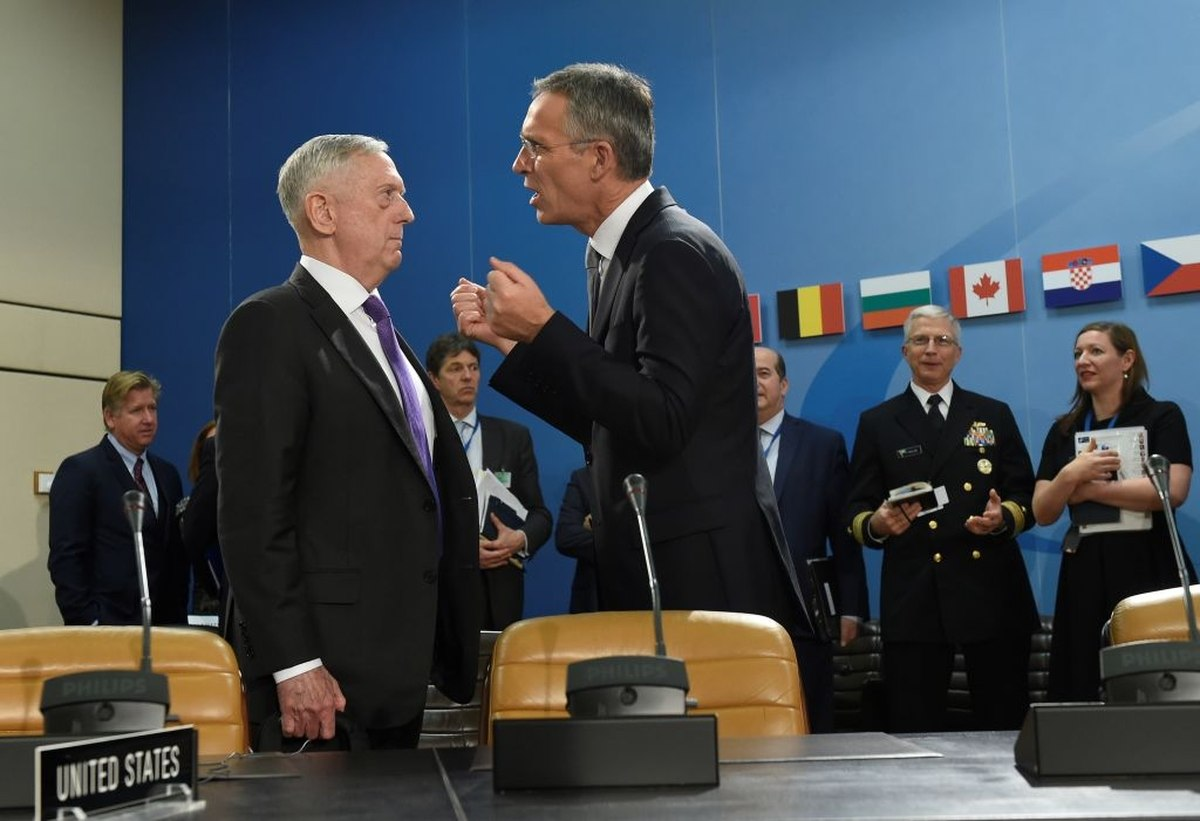
\includegraphics[width=0.95\textwidth]{mattis-nato.jpg}
	\label{fig:mattis-nato}
\end{figure}


\end{frame}

%------------------------------------------------

\begin{frame}[standout]

\huge \textit{Does alliance participation increase military spending?} \uncover<2->{Or decrease it?}

 \end{frame}

%------------------------------------------------

\begin{frame}{Competing Results}

\begin{table}[hbt!]
\begin{center}
\begin{tabular}{lccc}
     & Decrease & Increase & Null \\
\hline
Most \& Siverson 1987  &  &  & X \\
Conybeare 1994 & X & &  \\
Diehl 1994 &  & X &  \\
Goldsmith 2003 &  &  & X \\
Morgan \& Palmer 2006 &  & X & \\ 
Quiroz-Flores 2011 &  & X &  \\ 
\hline
\end{tabular}
\end{center} 
\end{table}


 \end{frame}

%------------------------------------------------

\begin{frame}{Omission: Alliance Heterogeneity}


\begin{itemize}
\item Alliances can \textit{increase or decrease} military spending. 
\pause
\item Depends on alliance characteristics. 
\end{itemize} 

\end{frame}

%------------------------------------------------
 \begin{frame}[standout]

Treaty depth is a key sources of differences between alliances. 

 \end{frame}


%------------------------------------------------

\begin{frame}{Outline}

I make my claim about alliance participation and military spending in three ways: 

\pause
\begin{enumerate}
\item Argument: Treaty Depth and Non-Major Powers
\pause
\item Statistical Analysis
\pause
\item Evidence from US alliances
\end{enumerate}


\end{frame}

%------------------------------------------------

\section{Argument}


%------------------------------------------------

\begin{frame}{The Problem of Free-riding}

Alliances are a form of international cooperation. Free-riding means alliance members:

\begin{enumerate} 
\pause
\item Rely on partners for protection and  
\pause
\item Reduce defense spending.
\end{enumerate}  

\end{frame}

%------------------------------------------------

\begin{frame}[standout]

Deep alliances restrain free-riding.   

\end{frame}

%------------------------------------------------

\begin{frame}{Treaty Depth}

Deep treaties stipulate extensive defense cooperation. 

\begin{enumerate} 
\pause
\item \textbf{Primary Obligations} 
\begin{itemize}
\item Whether the alliance promises military support and conditions on that support. 
\end{itemize}
\pause
\item \textbf{Formal defense cooperation}:
\pause
\begin{itemize}
\item Bases, policy coordination, military aid, side agreements, formal institutions. 
\end{itemize}  
\end{enumerate}  

\end{frame}


%------------------------------------------------

\begin{frame}{Limits on Free-Riding}

There are two ways depth limits alliance members ability to free-ride. 

\begin{enumerate}
\pause
\item Greater alliance value.   
\pause
\item Greater allied leverage. 
\end{enumerate}

\end{frame}

%------------------------------------------------

\begin{frame}[standout]

Depth is relevant for non-major powers because they are more prone to free-ride. 

\end{frame}


%------------------------------------------------

\begin{frame}{Non-Major Powers}

\begin{itemize}
\item Emphasize immediate security.
\pause
\item Constraint: Opportunity Costs of Military Spending.  
\pause
\item Alliance participation usually \emph{decreases} military spending. 
\end{itemize} 

\end{frame}

%------------------------------------------------

\begin{frame}[standout]

\begin{quote}
\textsc{Hypothesis 1}: As alliance treaty depth increases, growth in non-major power military spending from alliance participation will increase. 
\end{quote} 


\end{frame}

%------------------------------------------------

\section{Empirical Analysis} 

%-----------------------------------------------

\begin{frame}{Research Design}

I need two things to test the prediction: 

\pause 
\begin{enumerate} 
\item Measure of treaty depth--- measurement model. 
\pause
\item Connect alliance-level variation with state-level outcomes--- multilevel analysis.  
\end{enumerate} 


\end{frame}

%------------------------------------------------

\begin{frame}{Measuring Treaty Depth}

I use a latent variable model to infer treaty depth from observed promises. 

\pause 

My measure of depth for each alliance is the posterior mean of a latent factor. 

\end{frame} 

%------------------------------------------------

\begin{frame}{Details of Measure}
 
\begin{itemize}
\item Multiple observed indicators of depth (ATOP): 
\begin{itemize} 
\item \textit{Primary Obligations}: offense, defense, neutrality, consultation, non-aggression, unconditional military support.
\item \textit{Defense Cooperation}: bases, integrated command, military aid, IO formation, defense policy coordination, other military agreements. 
\end{itemize} 
\pause 
\item Semiparametric mixed factor analysis. (Murray et al 2013)
\pause
\item Generates a posterior distribution of depth for each alliance.
\end{itemize} 


\end{frame} 

%------------------------------------------------

\begin{frame}{Latent Measure of Treaty Depth}

% Visual summary of latent measure
\begin{figure}[htbp]
	\centering
		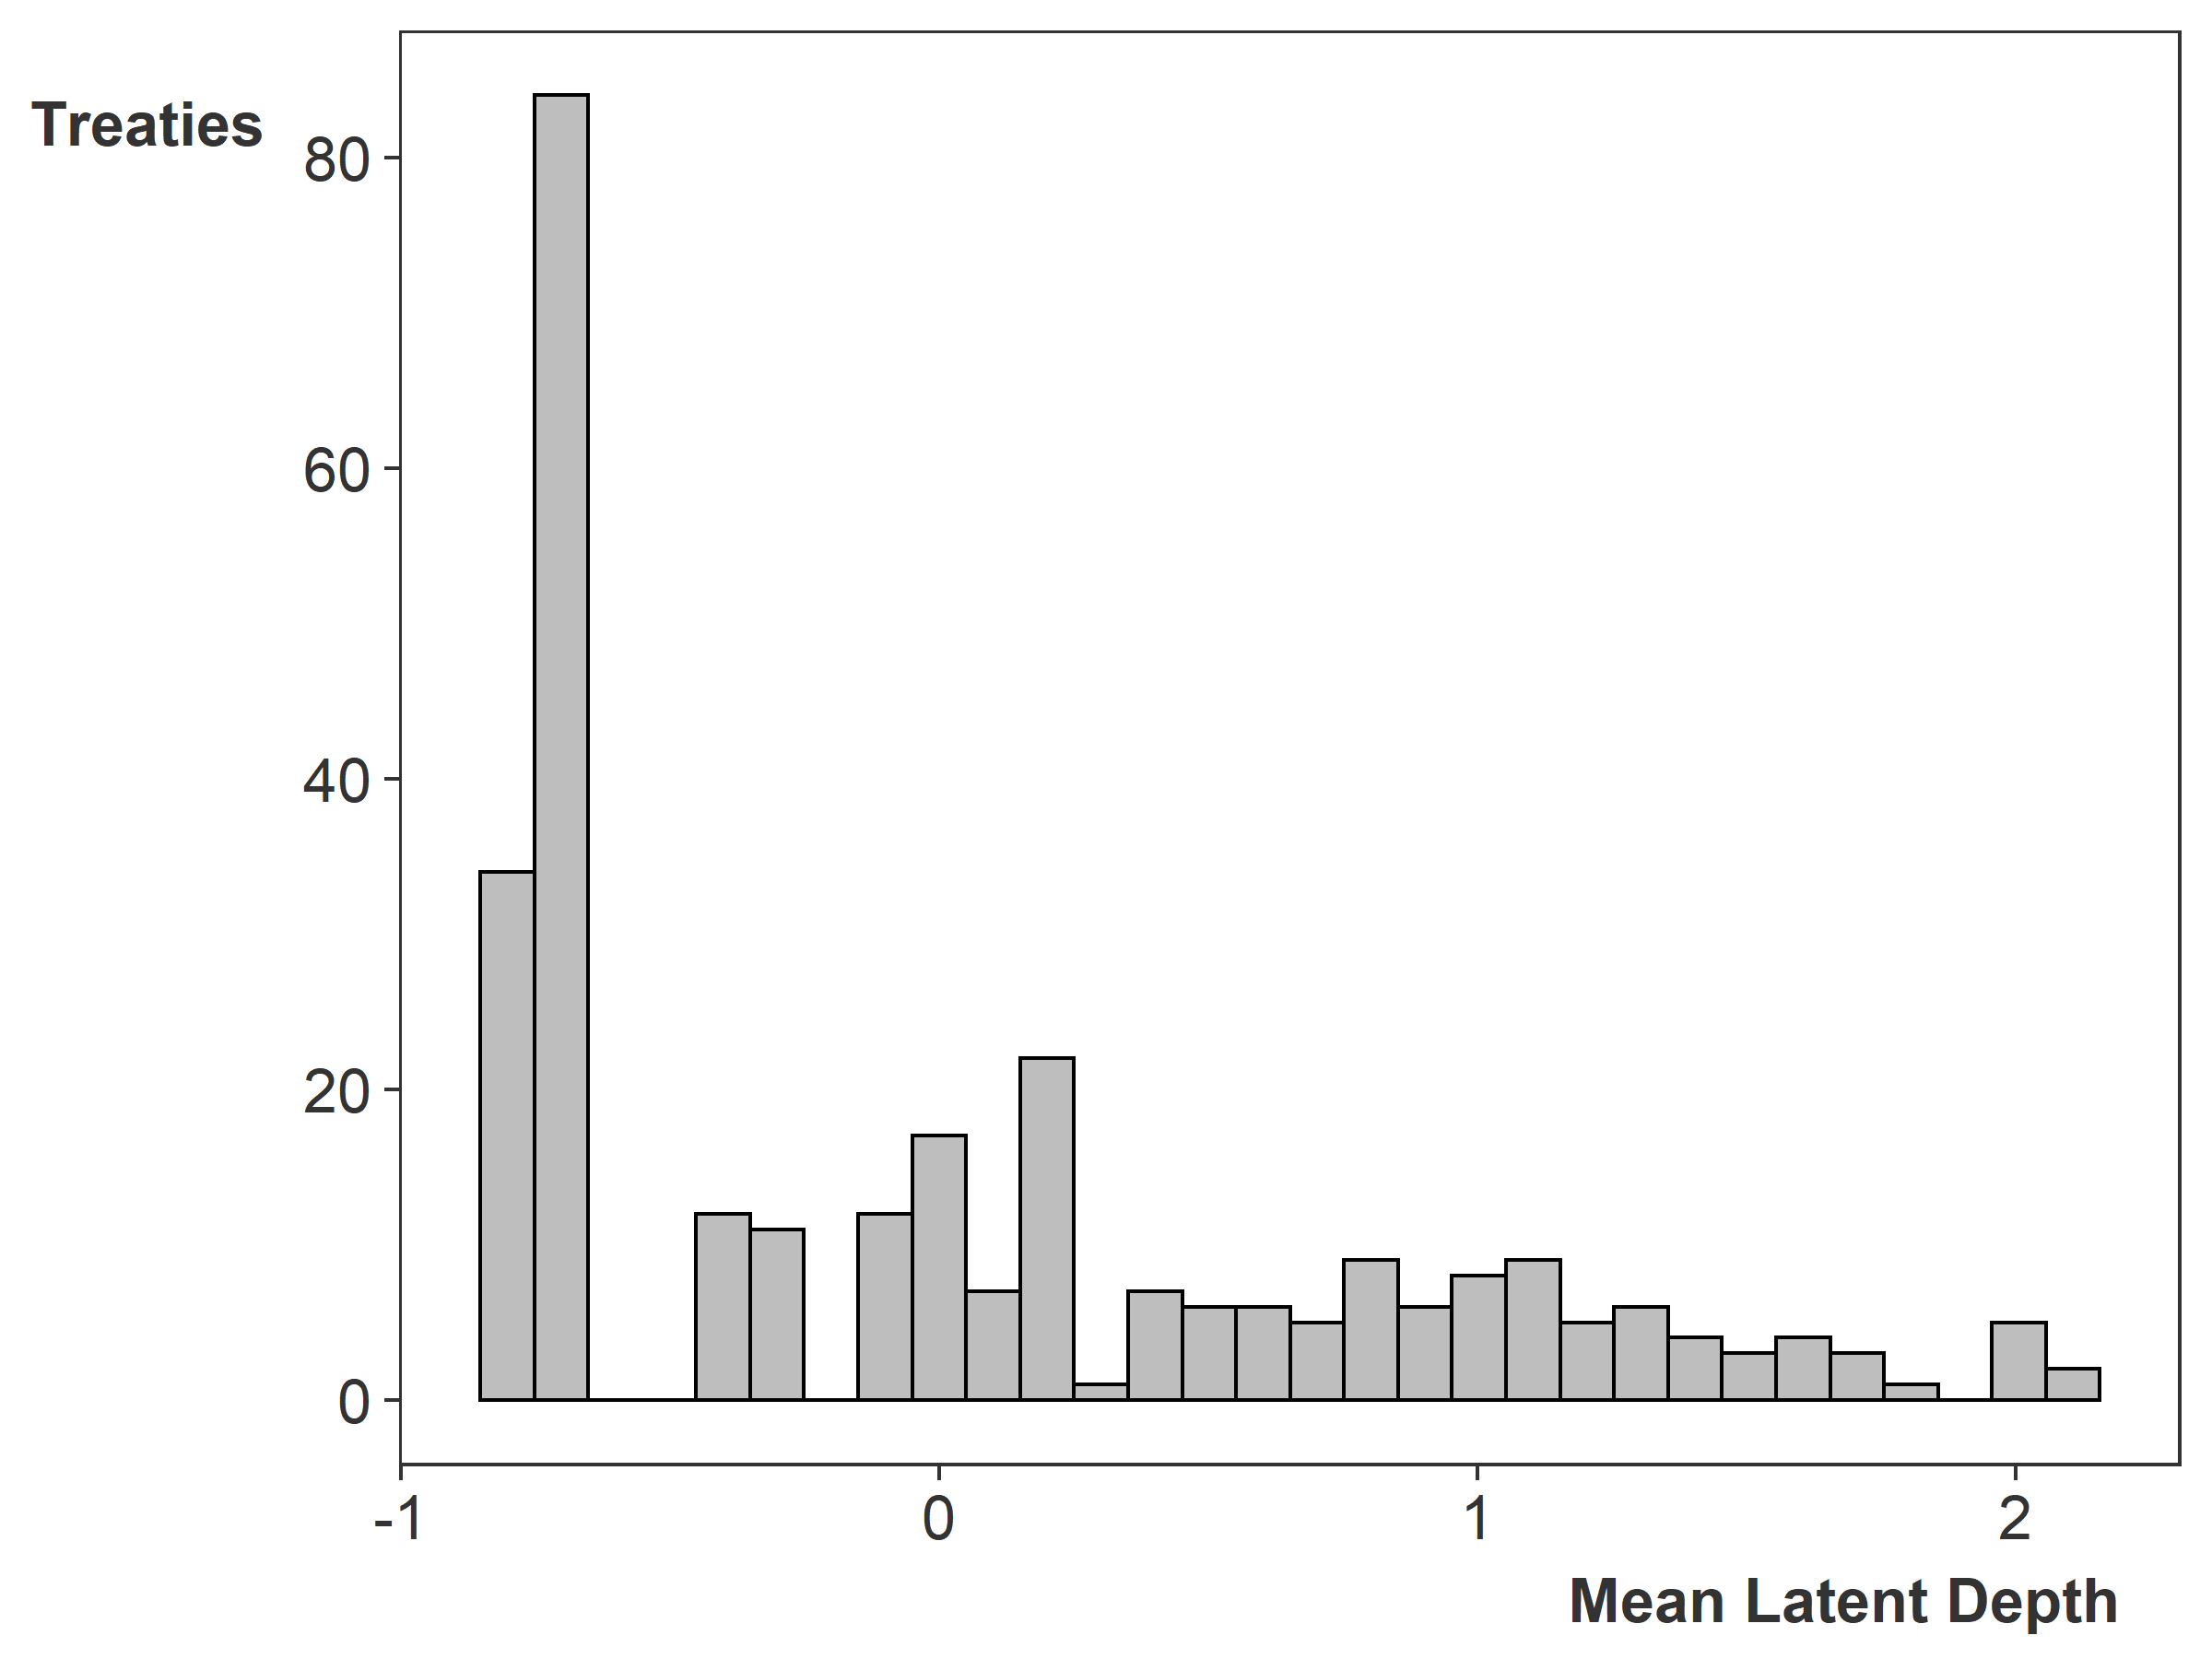
\includegraphics[width=0.95\textwidth]{ld-hist.png}
\end{figure}


\end{frame} 

%------------------------------------------------

\begin{frame}{Latent Measure of Treaty Depth: Shallow}

% Visual summary of latent measure
\begin{figure}[htbp]
	\centering
		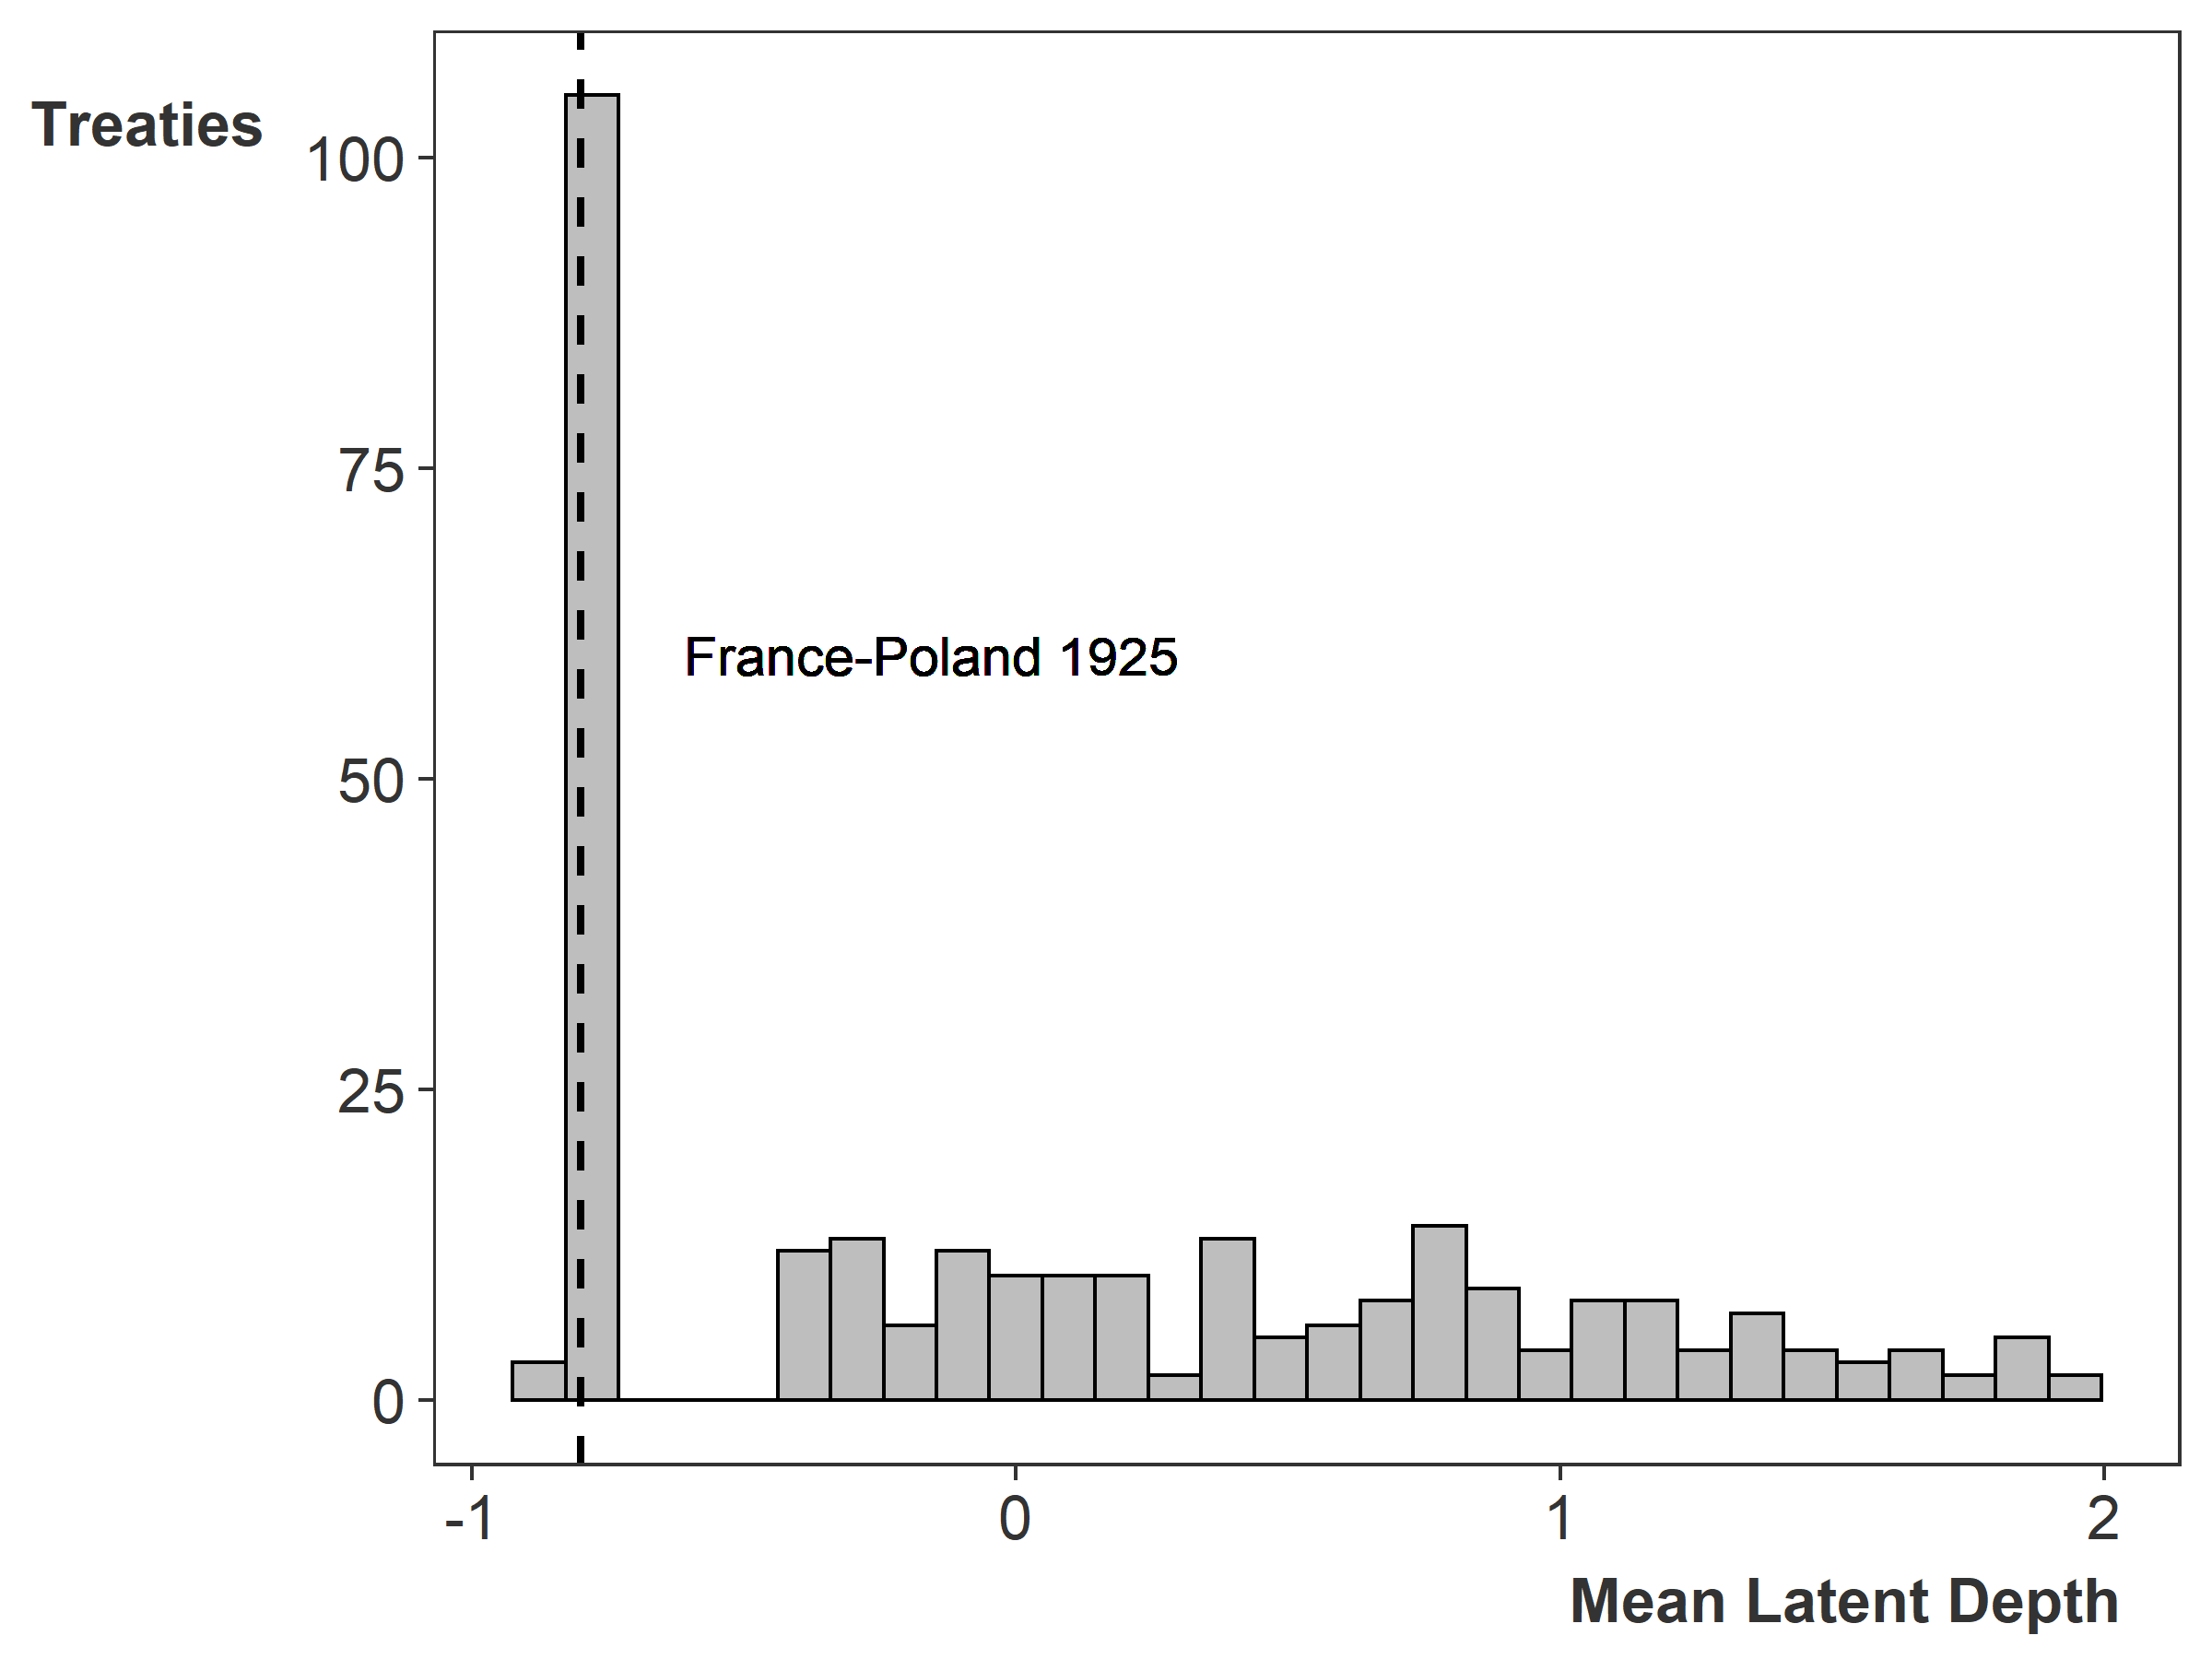
\includegraphics[width=0.95\textwidth]{ld-hist-shallow.png}
\end{figure}


\end{frame} 

%------------------------------------------------

\begin{frame}{Latent Measure of Treaty Depth: Typical}

% Visual summary of latent measure
\begin{figure}[htbp]
	\centering
		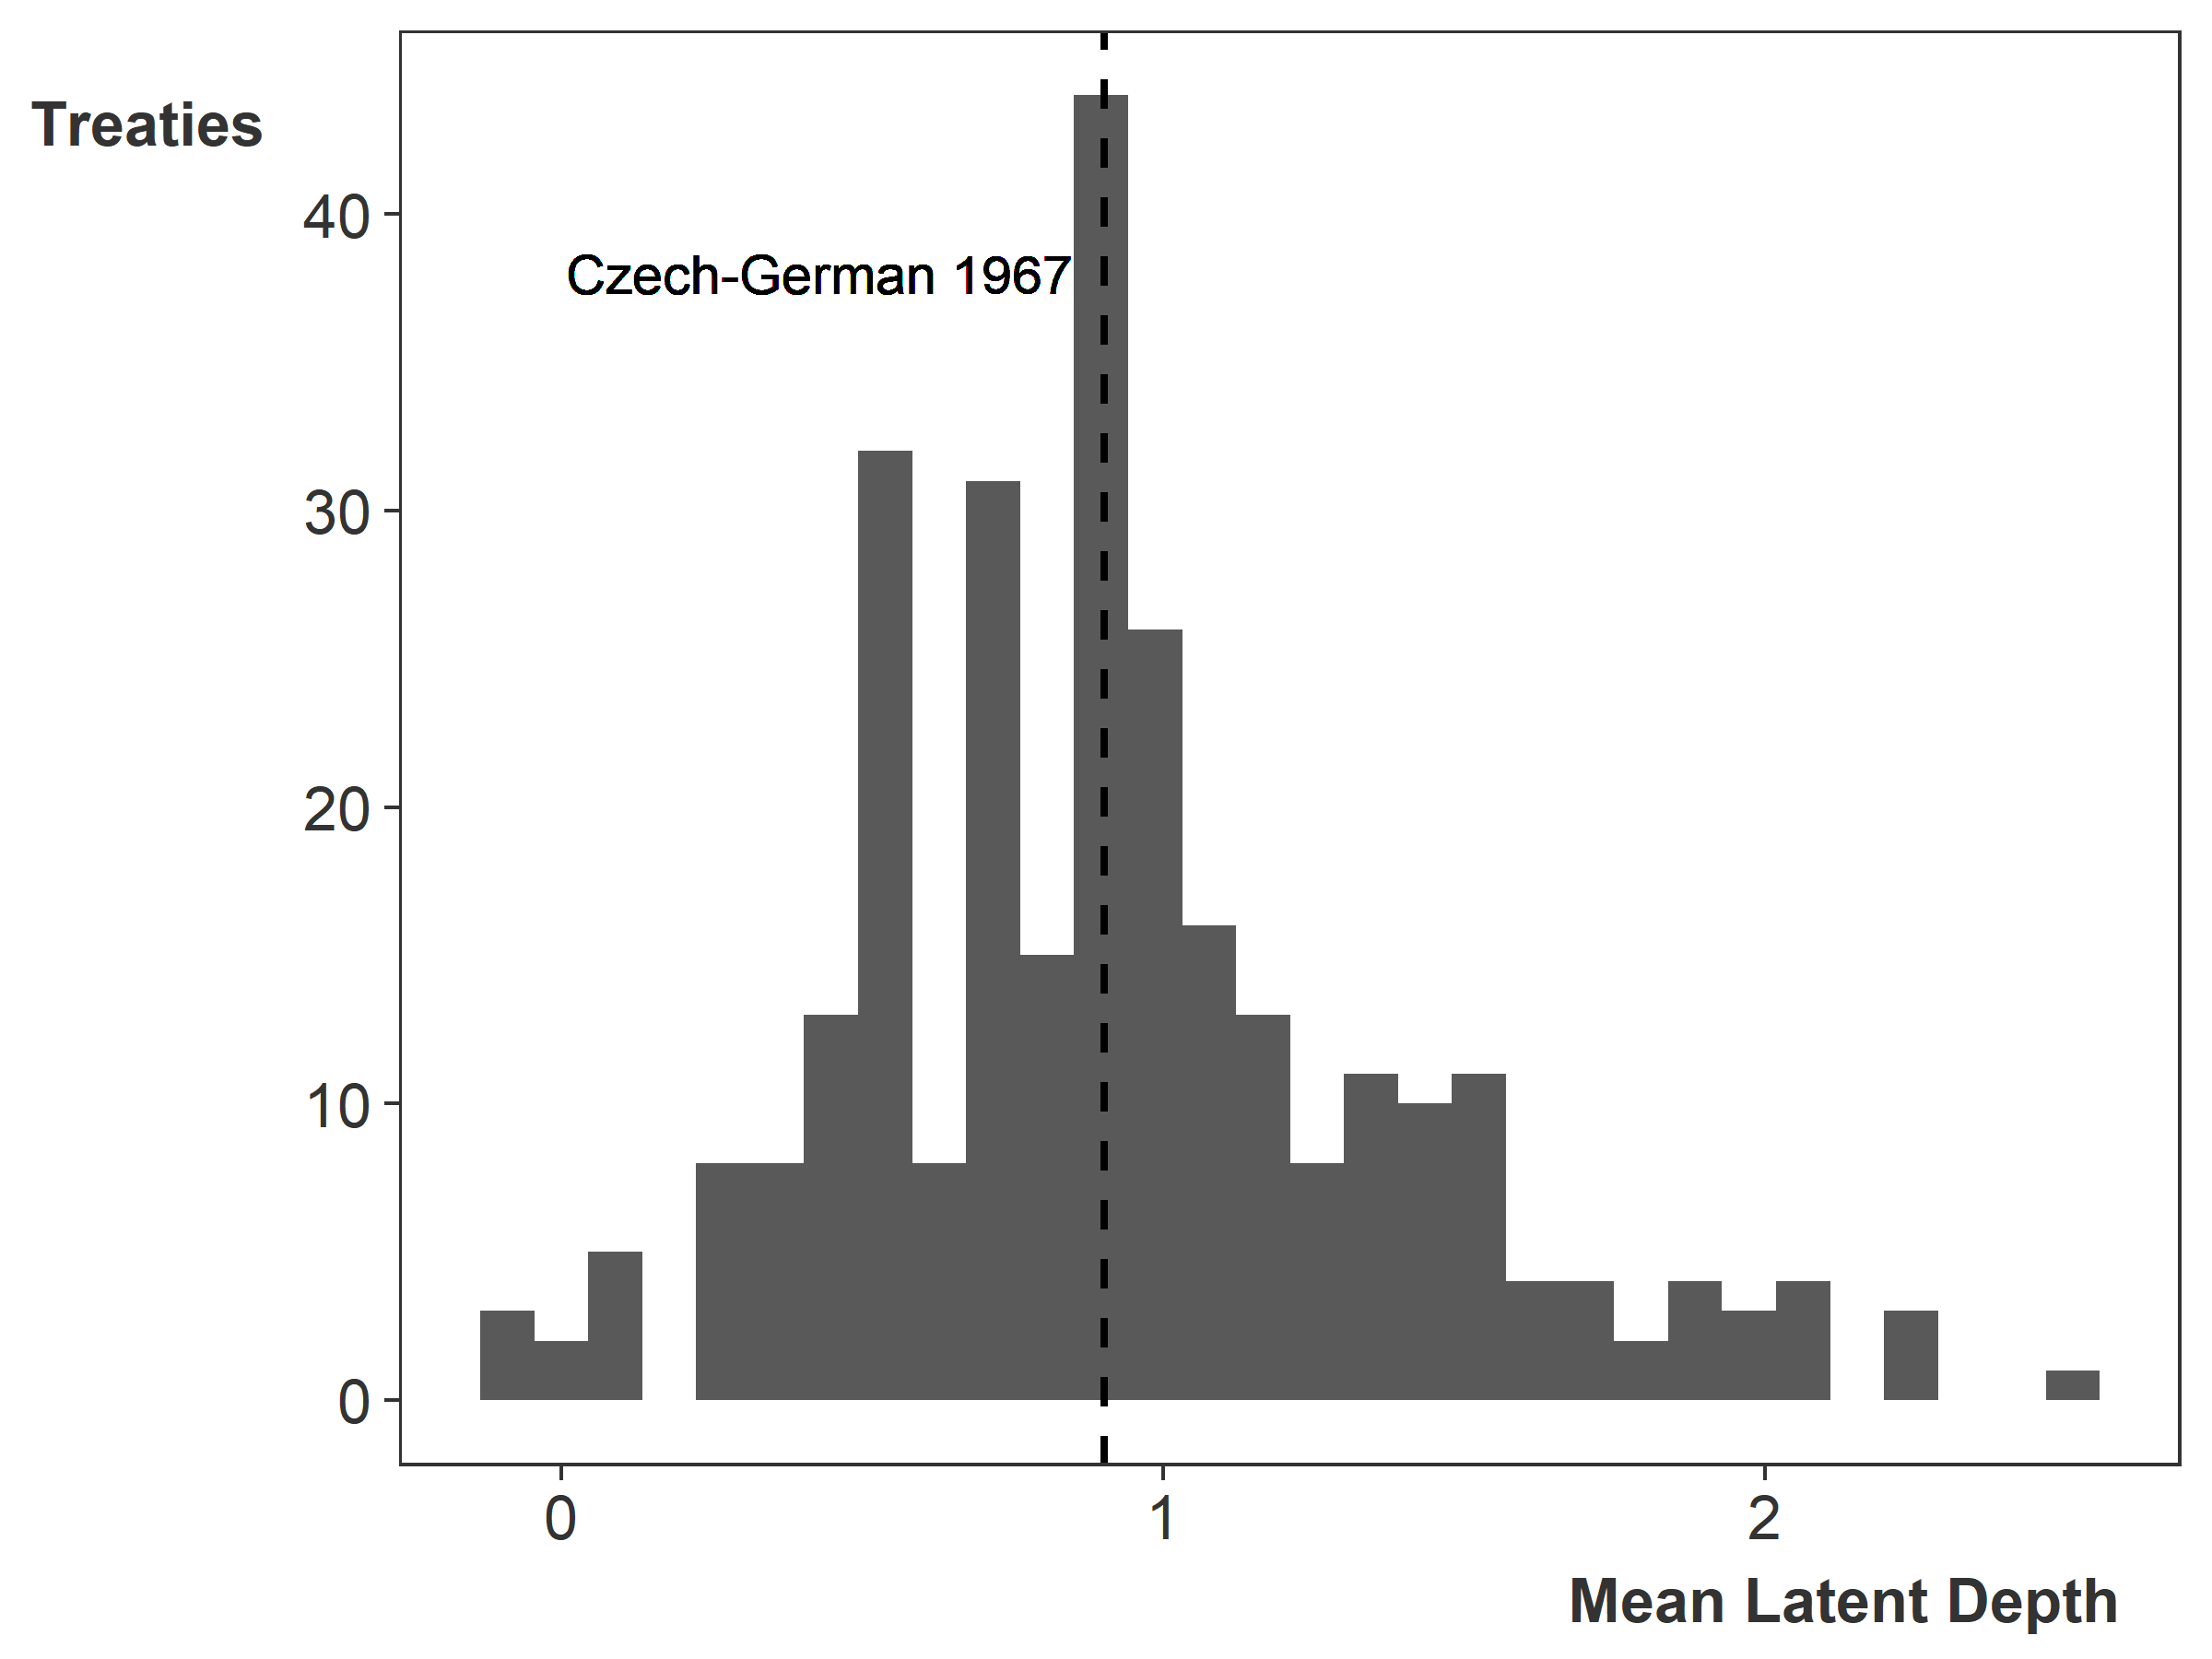
\includegraphics[width=0.95\textwidth]{ld-hist-median.png}
\end{figure}


\end{frame} 

%------------------------------------------------

\begin{frame}{Latent Measure of Treaty Depth: Deep}

% Visual summary of latent measure
\begin{figure}[htbp]
	\centering
		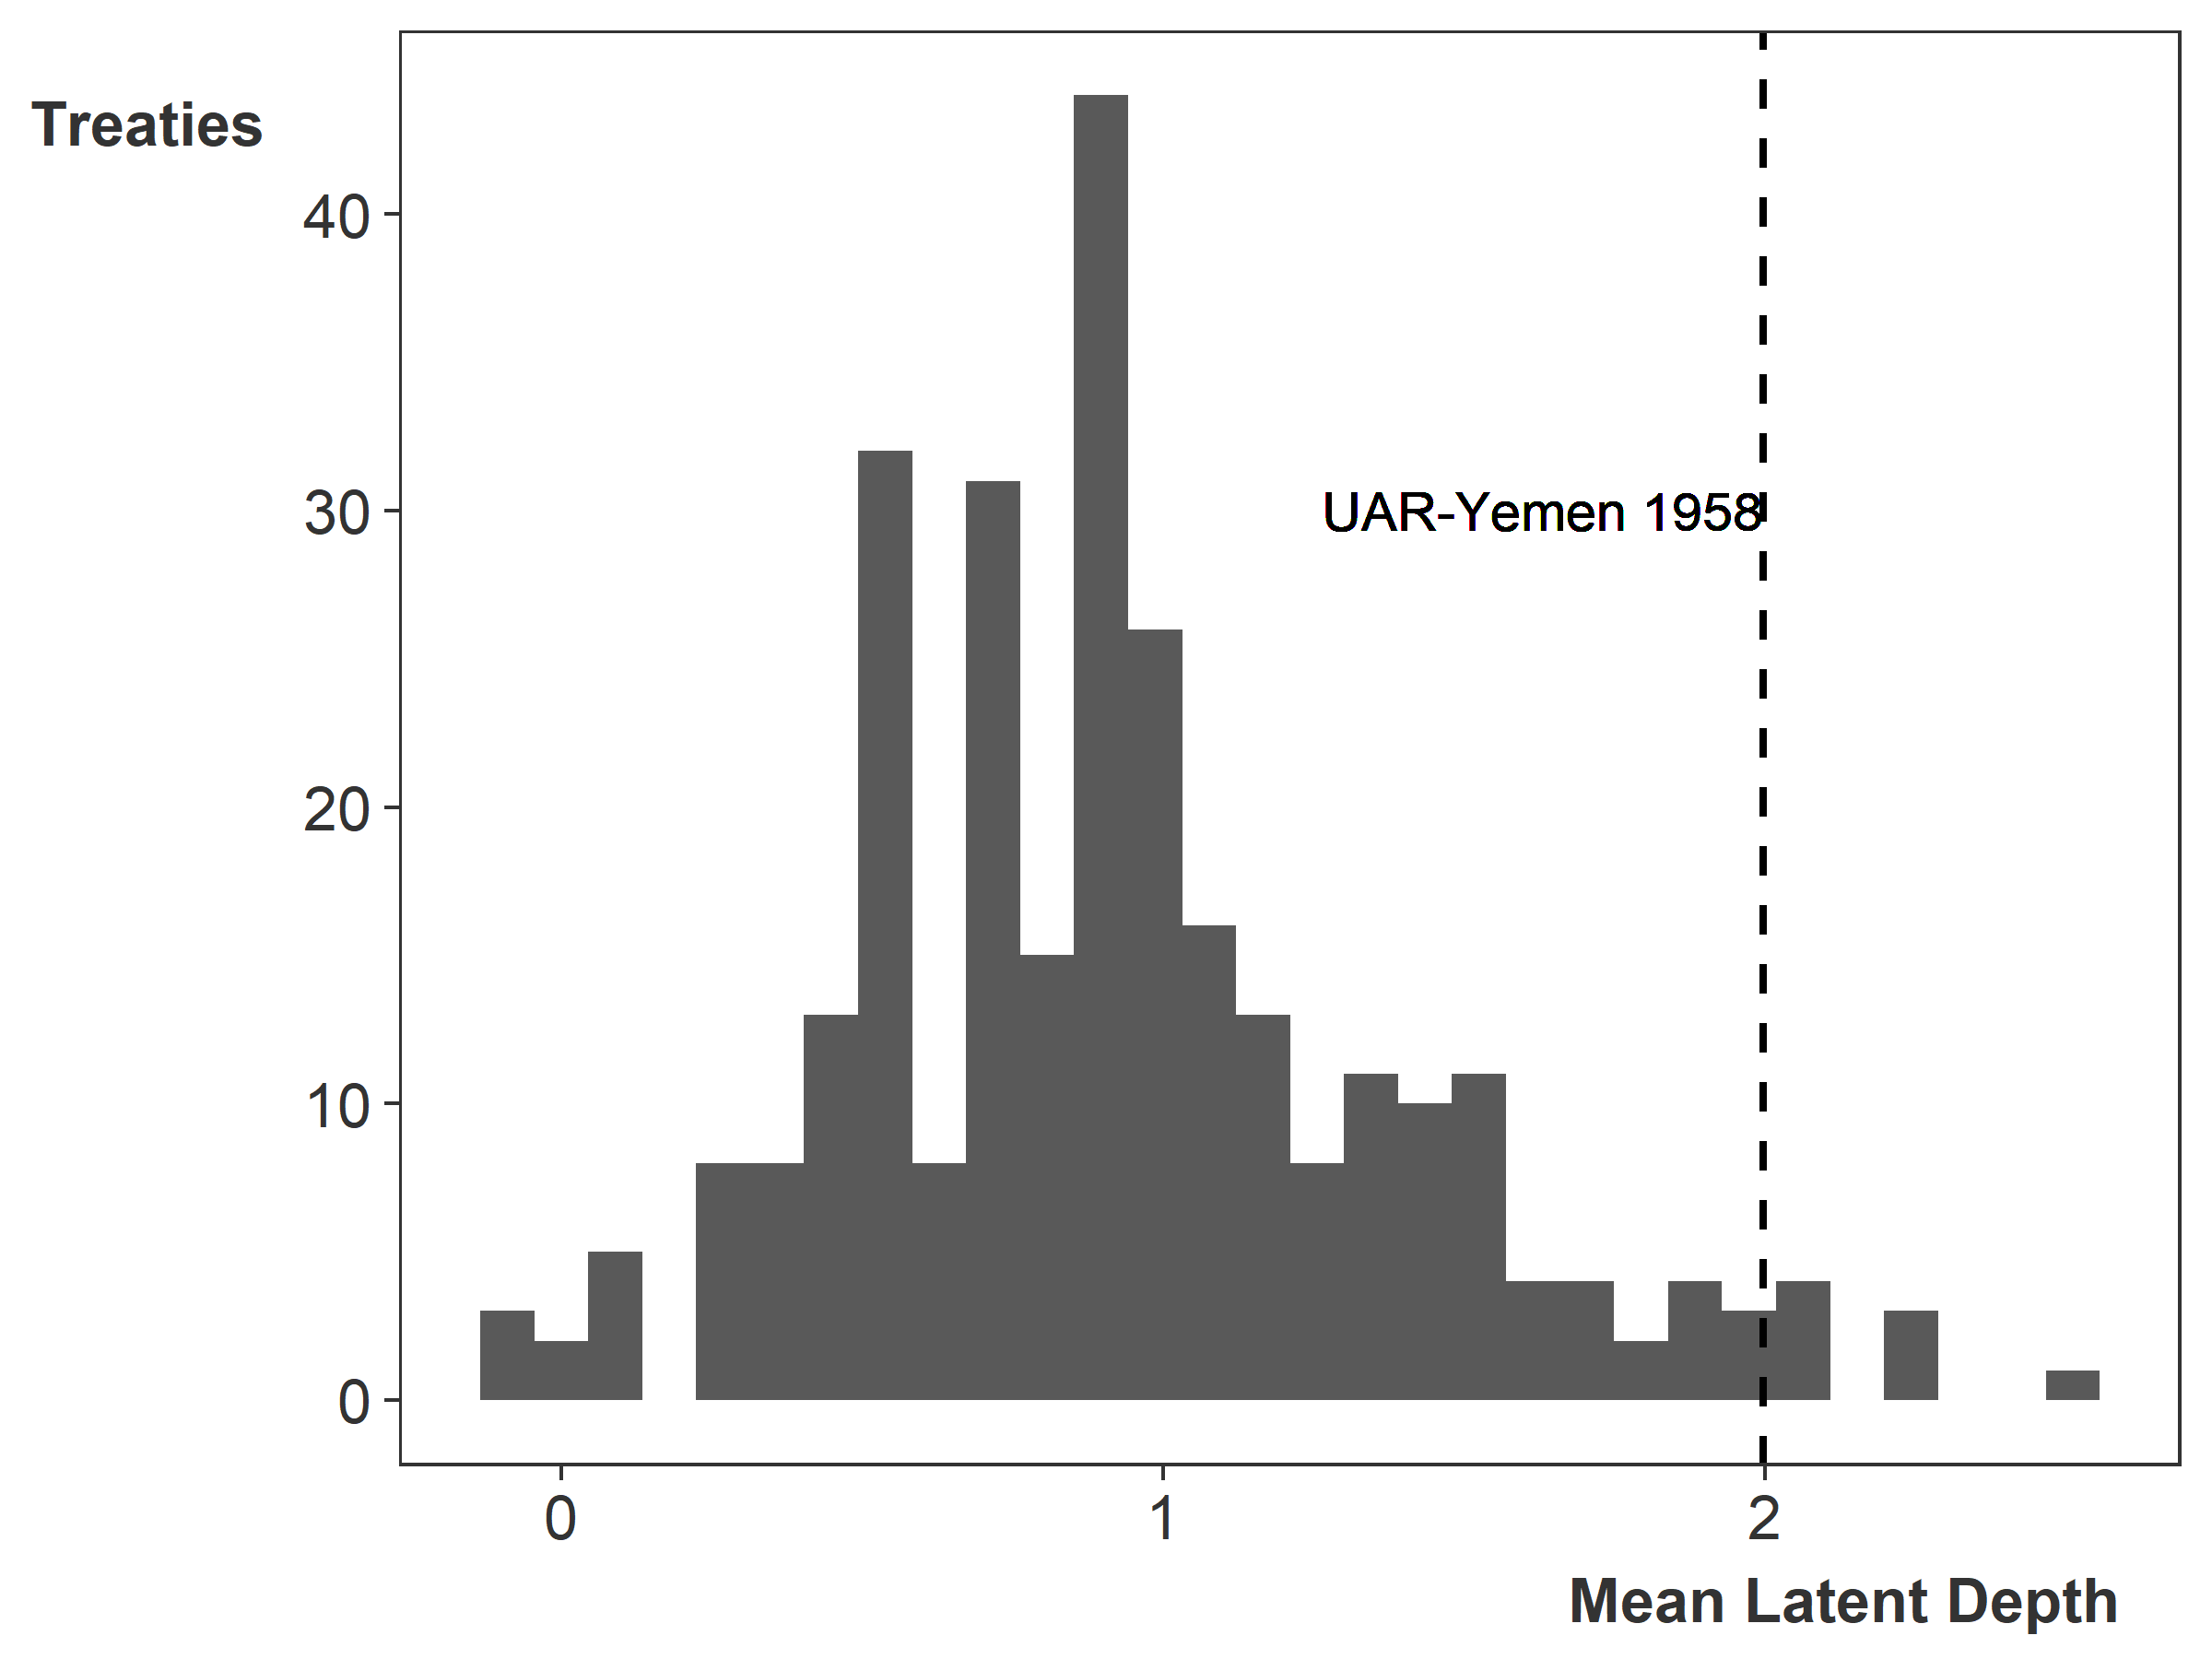
\includegraphics[width=0.95\textwidth]{ld-hist-deep.png}
\end{figure}


\end{frame} 


%------------------------------------------------

\begin{frame}{Empirical Analysis: Multilevel Model}

\begin{itemize} 
\item Link alliance-level variation with state-level outcomes. 
\pause
\item Two connected regressions: alliance and state-level. 
\pause 
\item Alliance characteristics modify the association between alliance membership and spending growth.  
\end{itemize} 

\end{frame} 


%------------------------------------------------

\begin{frame}{ML Model}

\[
\begin{array}{cccccc}
\uncover<2->{ & & & & &\mbox{Alliance} \\
& & & & &    \mbox{Characteristics}  \\
\uncover<3->{& & & & \lambda = & \alpha_{all} + \beta_1 \mbox{Depth} + \textbf{X} \beta \\}
& & & & &    \downarrow  \\}
\mbox{Growth} =     & \mbox{Varying}   & + & \mbox{State}   & + & \mbox{Alliance} \\
\mbox{Mil. Ex.}      & \mbox{Intercepts}&   &  \mbox{Vars.} &   & \mbox{Participation} \\
\uncover<3->{\mbox{y} = & \alpha + \alpha^{st} + \alpha^{yr}   & + & \textbf{W} \gamma  & + & \textbf{Z} \lambda \\}
\end{array}
\]


\end{frame}

%------------------------------------------------


\begin{frame}{ML Model Specification}

\begin{equation}
y \sim student_t(\nu, \mu, \sigma)
\end{equation}
\begin{equation}
\mu = \alpha + \alpha^{st} + \alpha^{yr} +\textbf{W}_{n \times k} \gamma + \textbf{Z}_{n \times a} \lambda
\end{equation}

\begin{equation}
\lambda_{a} \sim N(\theta_{a}, \sigma_{all})
\end{equation}
\begin{equation}
\theta_a = \alpha_{all} + \beta_1 \mbox{Treaty Depth} + \textbf{X}_{a \times l} \beta
\end{equation}


\end{frame}


%------------------------------------------------

\begin{frame}{Example}

\setbeamercovered{transparent}

\begin{equation*}
\uncover<2->{\mu_{it} =} \uncover<3>{\alpha} \uncover<4>{+ \alpha^{st} + \alpha^{yr}} \uncover<5>{+ W_{it} \gamma} \uncover<6>{+ Z_{it} \lambda}
\end{equation*}

Example year: Argentina 1955

\begin{equation*}
\begin{split}
& \uncover<2->{\mbox{1955 Growth Milex.} = } \uncover<3>{\mbox{Overall mean}} \\
& \uncover<4>{+ \mbox{Argentine Intercept} + \mbox{1955 Intercept}} \\
& \uncover<5>{+ \mbox{Argentine Characteristics}} \\
& \uncover<6>{+ \lambda_{OAS} * \mbox{OAS Expenditure} + \lambda_{Rio} * \mbox{Rio Pact Expenditure}}
\end{split}
\end{equation*}

\uncover<7>{
\begin{equation*}
\lambda_{Rio} = \alpha_{all} + \beta_1 0.34 + \mbox{Controls}
\end{equation*}
} 


\end{frame}


%------------------------------------------------


\begin{frame}[standout]{Z} 

\begin{tabular}{lccc}
State-Year & Rio Pact & Warsaw Pact & \ldots \\
\hline
Argentina 1954 & .347 & 0 & \ldots \\
Argentina 1955 & .418  & 0 & \ldots  \\
 \vdots & \vdots & \vdots & \ldots  
\end{tabular}

 \end{frame}



%------------------------------------------------

\begin{frame}{Sample and Key Variables}

\begin{itemize}
\item \textbf{Sample}: Non-major power states (COW)--- 1816-2007. 193 Alliances with military support. 
\pause
\item \textbf{DV}: Growth in military spending (COW) $ = \frac{ \Delta \mbox{Mil. Expend}_t }{ \mbox{Mil. Expend}_{t-1} }$ 
\pause
\begin{itemize} 
\item Transformed with Inverse Hyperbolic Sine. 
\end{itemize} 
\pause
\item \textbf{Alliance-Level IV}: Mean treaty depth
\end{itemize} 

\end{frame}


%------------------------------------------------

\begin{frame}{Controls}

\begin{itemize}
\item \textbf{State-Level Controls}: Interstate war, civil War, annual MIDs, GDP growth, POLITY, Cold War, rival military expenditures. 
\pause 
\item \textbf{Alliance-Level Controls}: Share of democracies, number of members, wartime, asymmetric obligations, US member (Cold War), USSR member.

\end{itemize} 

\end{frame}


%------------------------------------------------

\subsection{Results}

%------------------------------------------------

\begin{frame}{Association Between Treaty Depth and Growth in Military Spending} 

\begin{figure}
	\centering
		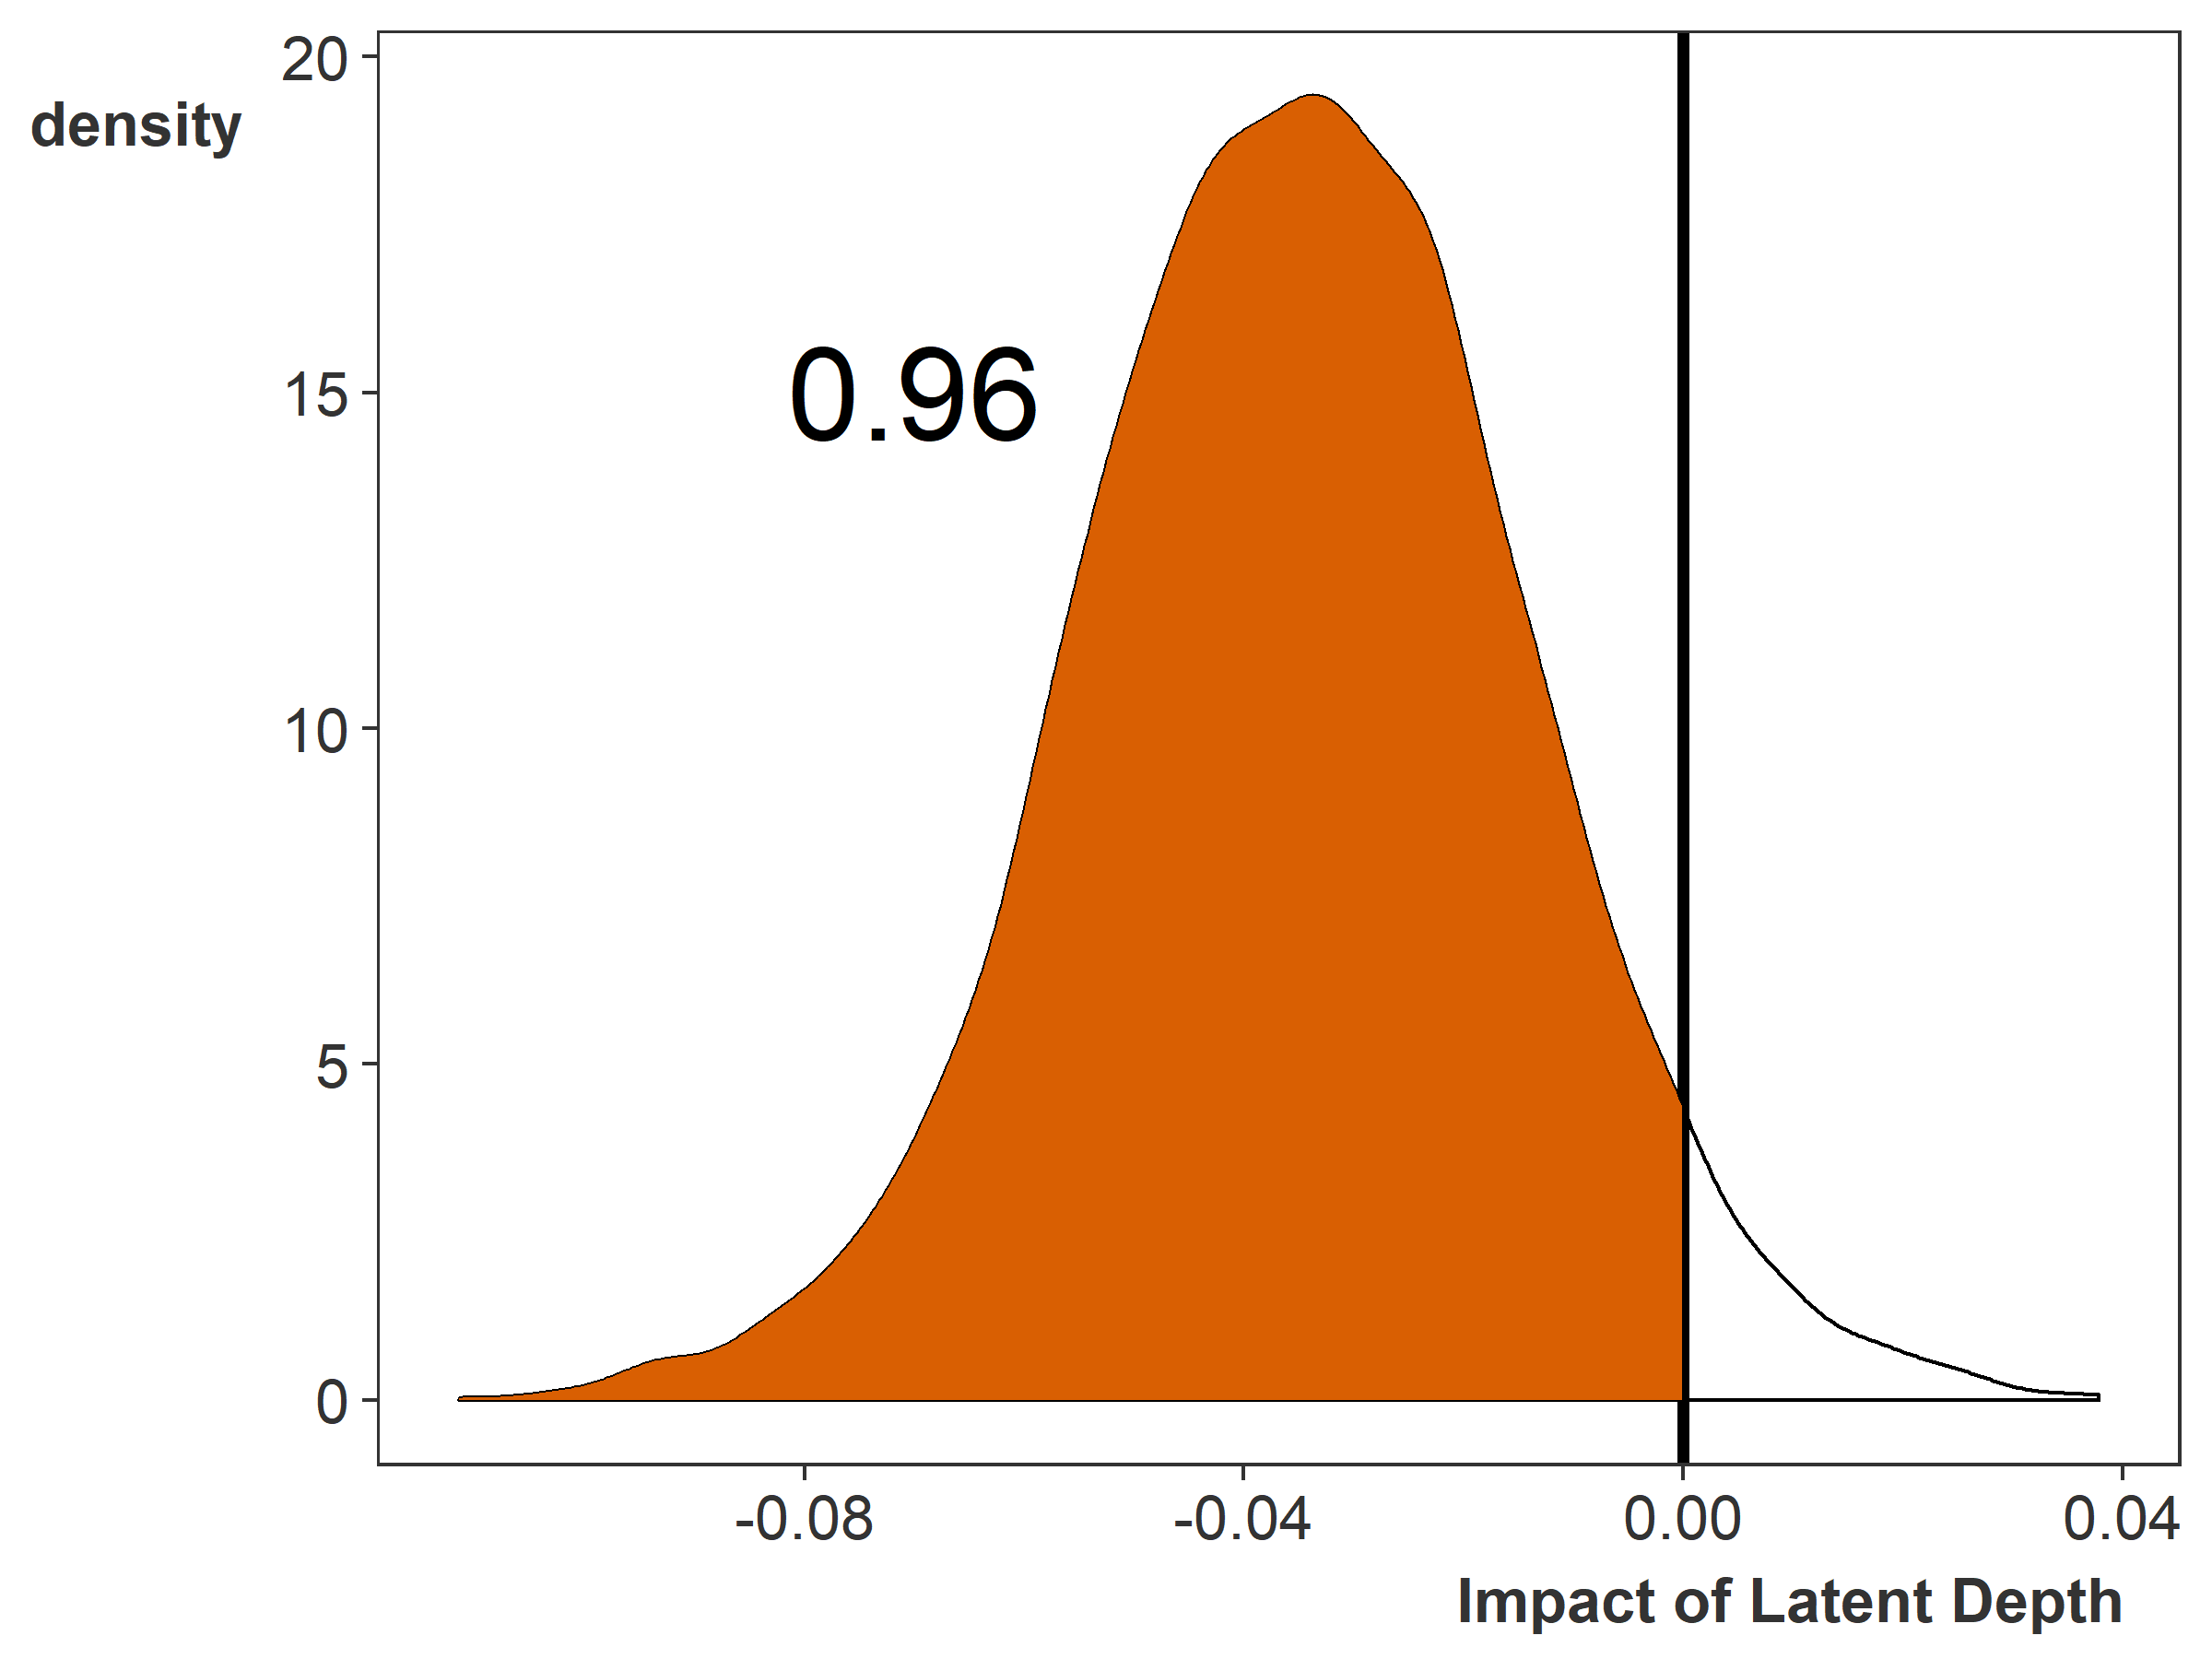
\includegraphics[width=0.90\textwidth]{depth-post.png}
	\label{fig:depth-post}
\end{figure}


\end{frame}


%------------------------------------------------

\begin{frame}[standout]{Importance} 

\begin{tabular}{cc}
 Post. Mean & Median Growth \\
\hline
\pause
 0.02 & 0.06  \\
\end{tabular}

\pause

US spent \$36.0 billion on NATO in 2018, or 5.5\% of the total defense spending. 


\end{frame}

%------------------------------------------------


\begin{frame}{Treaty Depth and $\lambda$}

\begin{figure}[htbp]
	\centering
		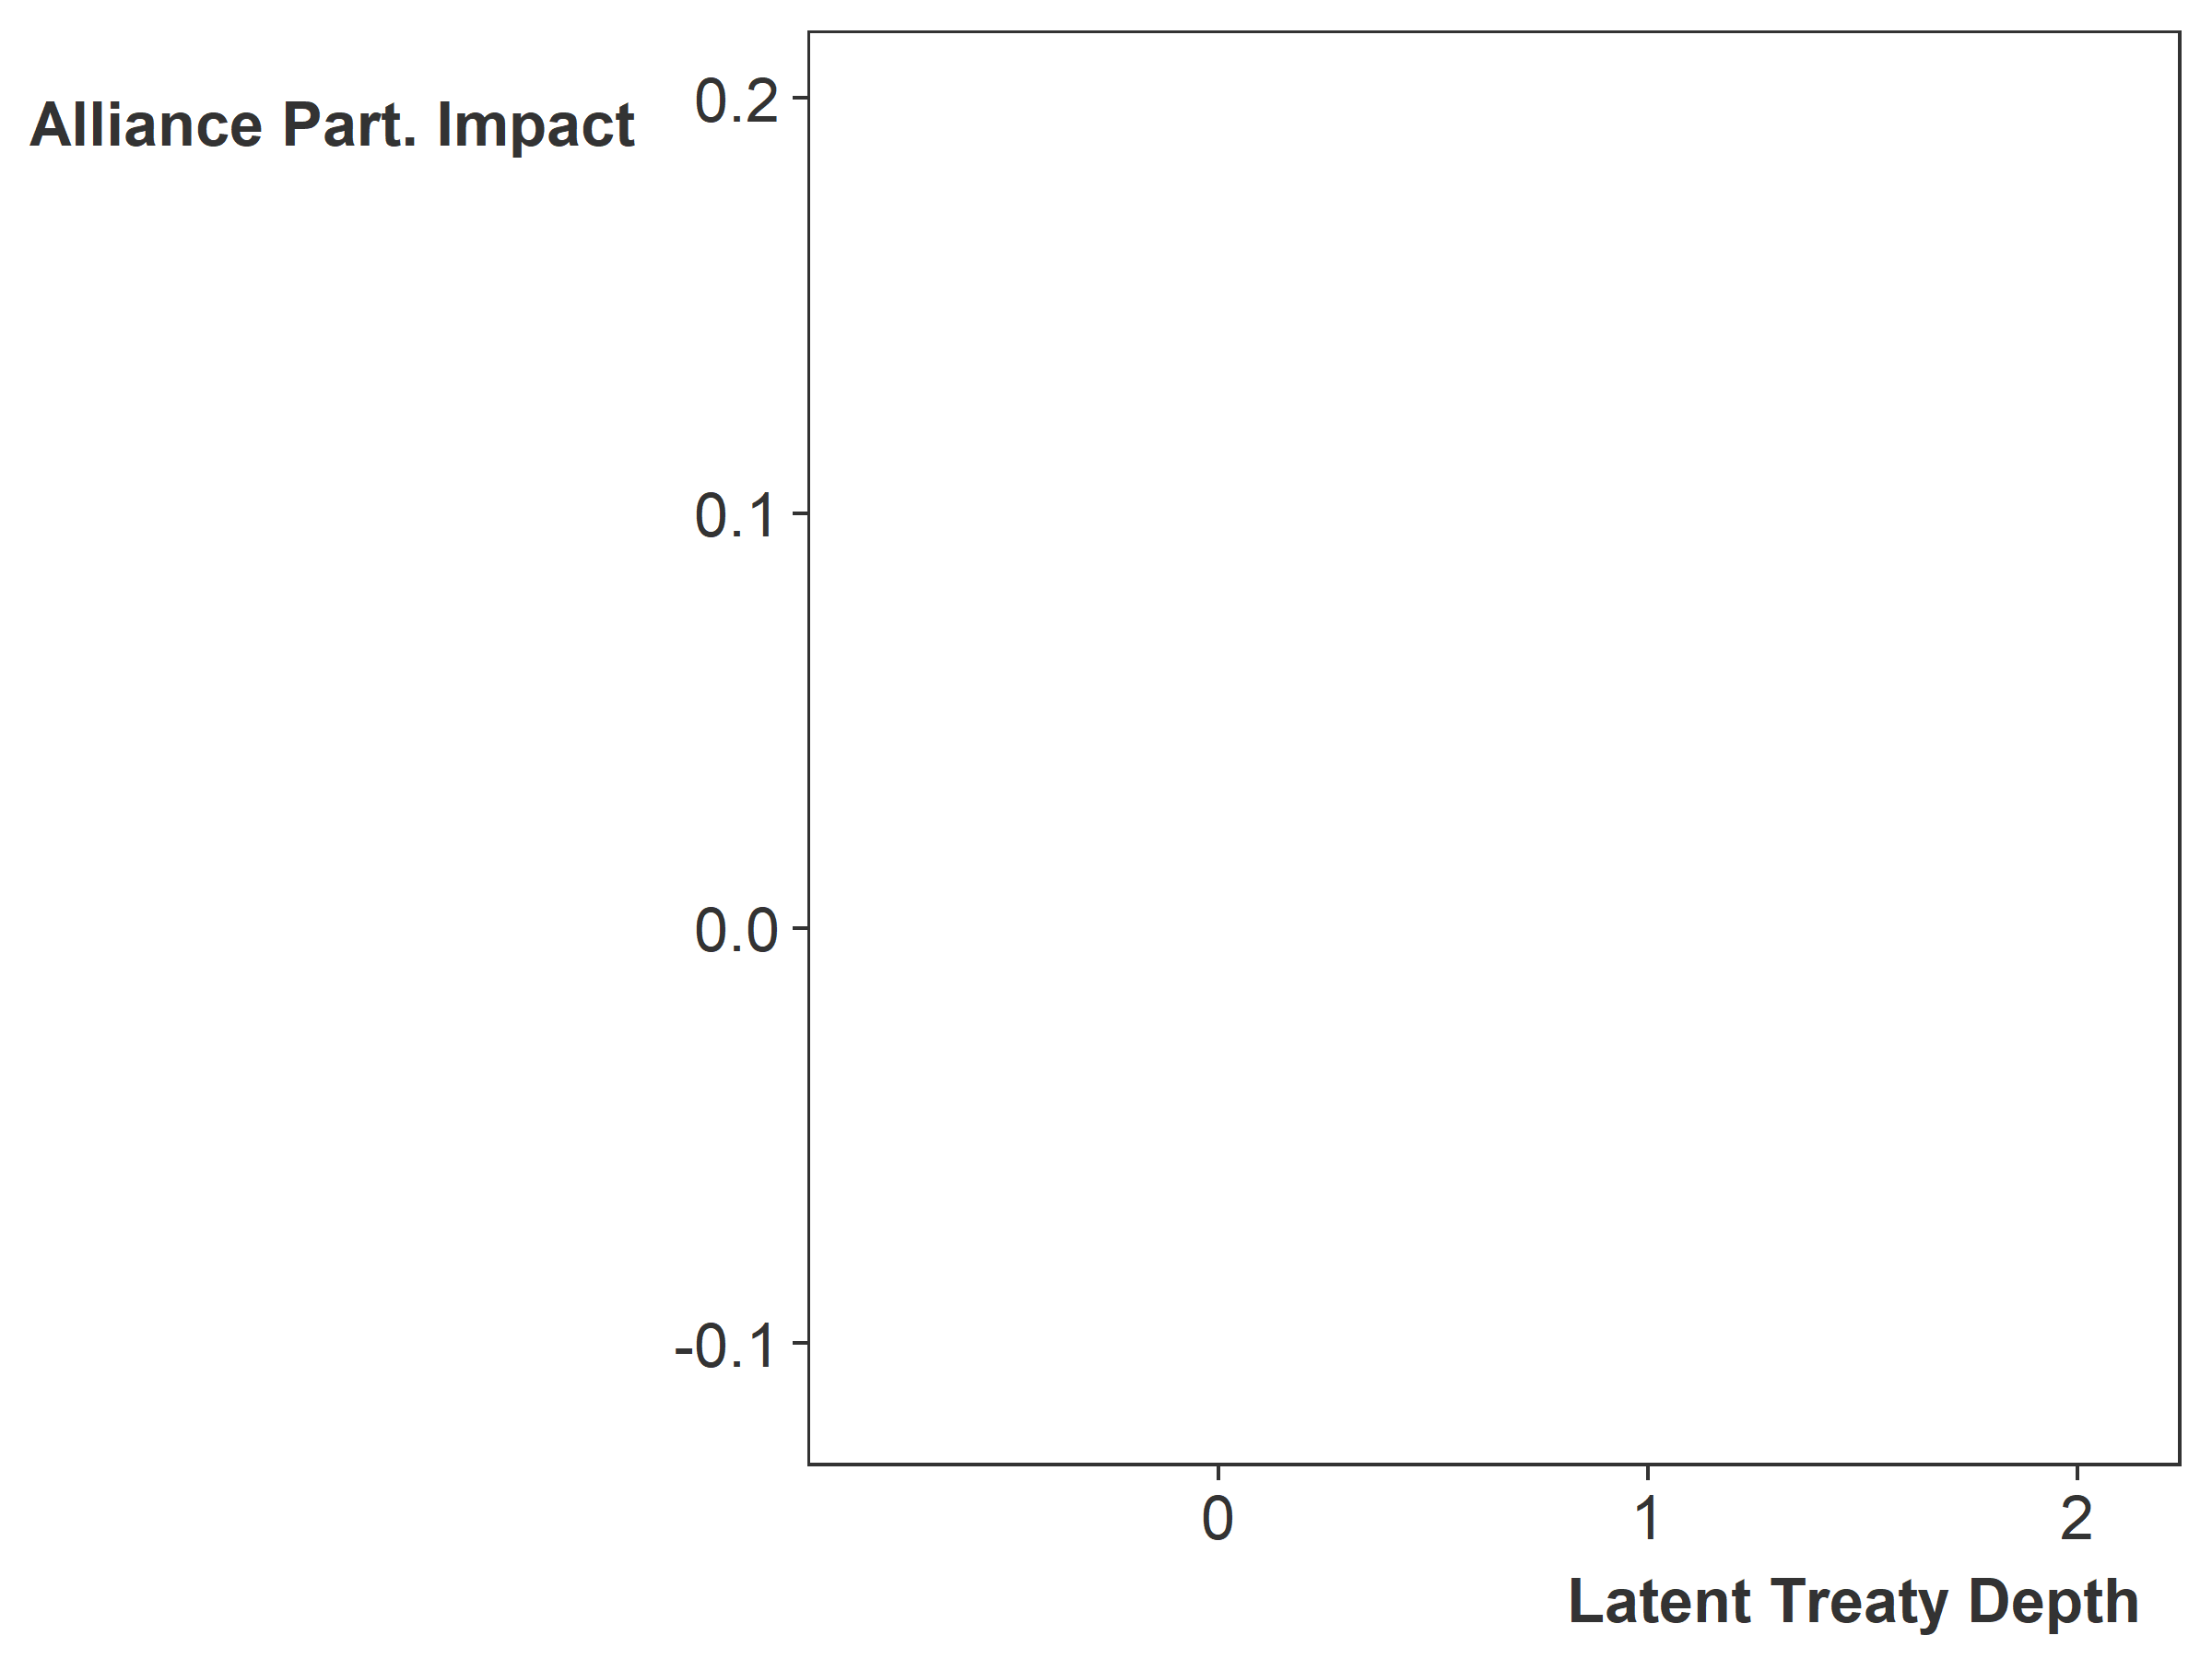
\includegraphics[width=0.95\textwidth]{ld-lambda-blank.png}
	\label{fig:ld-lambda-blank}
\end{figure}


\end{frame}


%------------------------------------------------

\begin{frame}{Treaty Depth and $\lambda$: Non-major Powers}

\begin{figure}
	\centering
		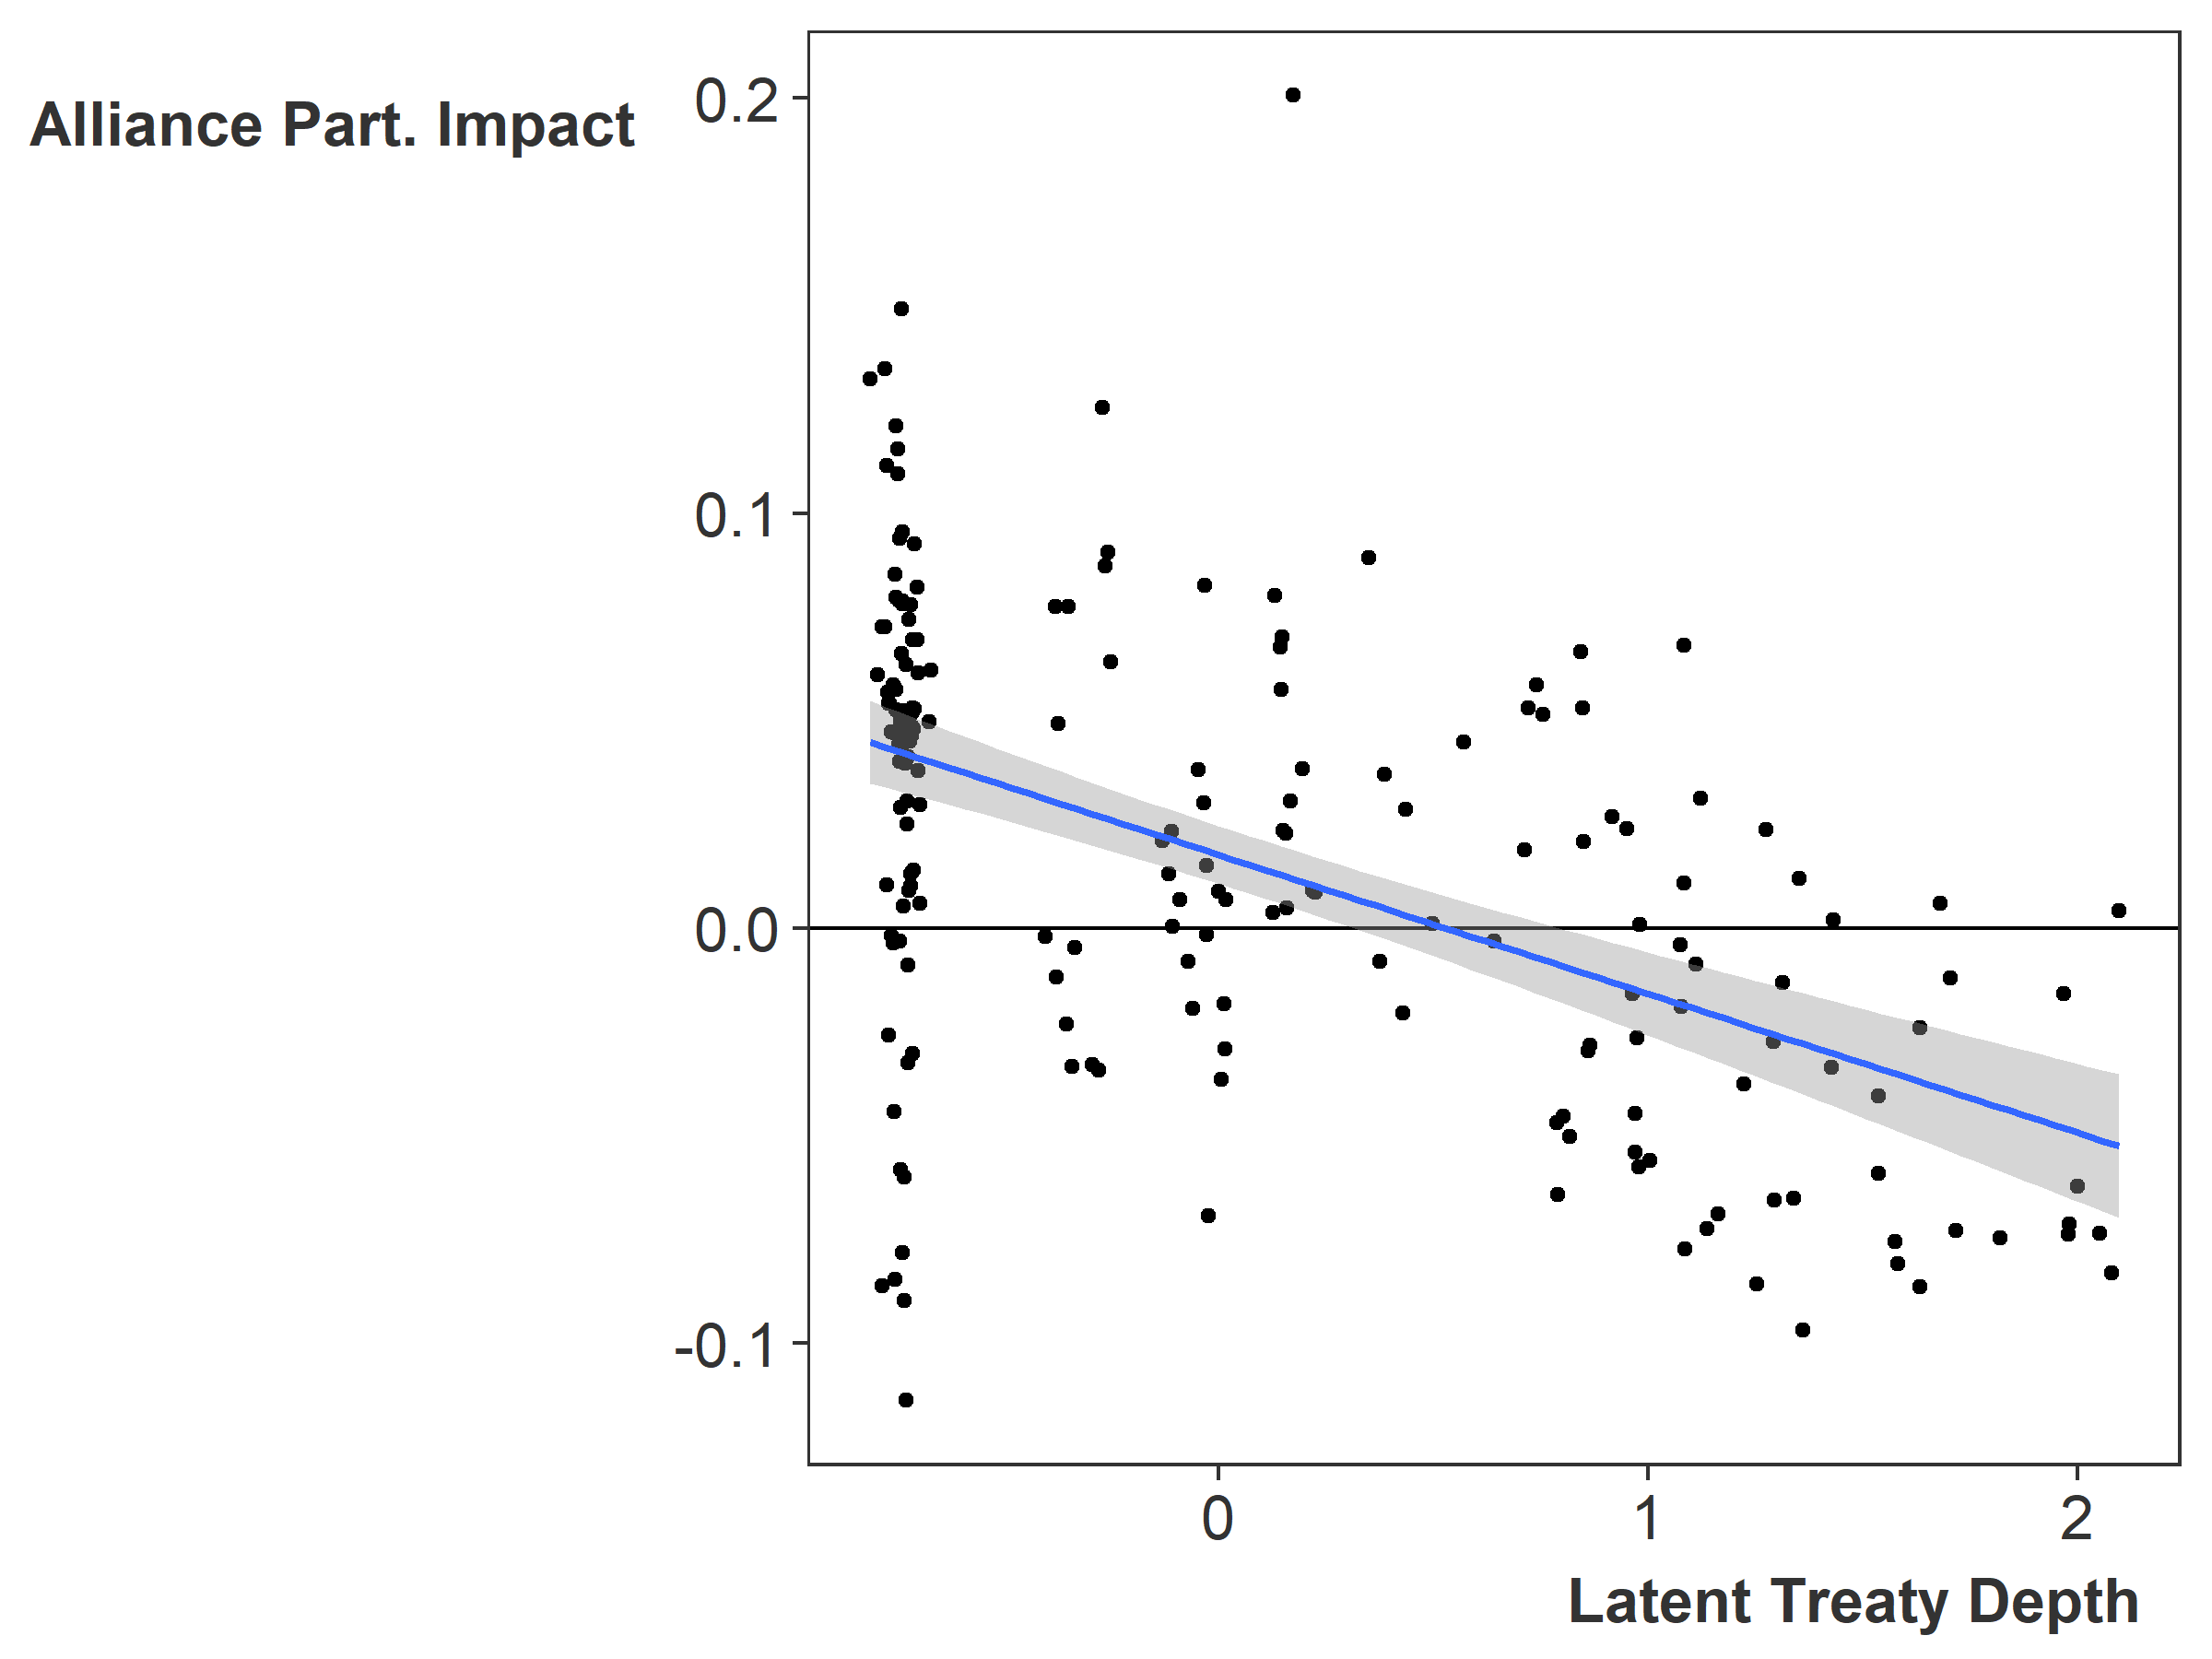
\includegraphics[width=0.9\textwidth]{ld-lambda-min.png}
	\label{fig:ld-lambda-min}
\end{figure}


\end{frame}


%------------------------------------------------

\begin{frame}{Treaty Depth and Other Alliance Characteristics}

\begin{figure}
	\centering
		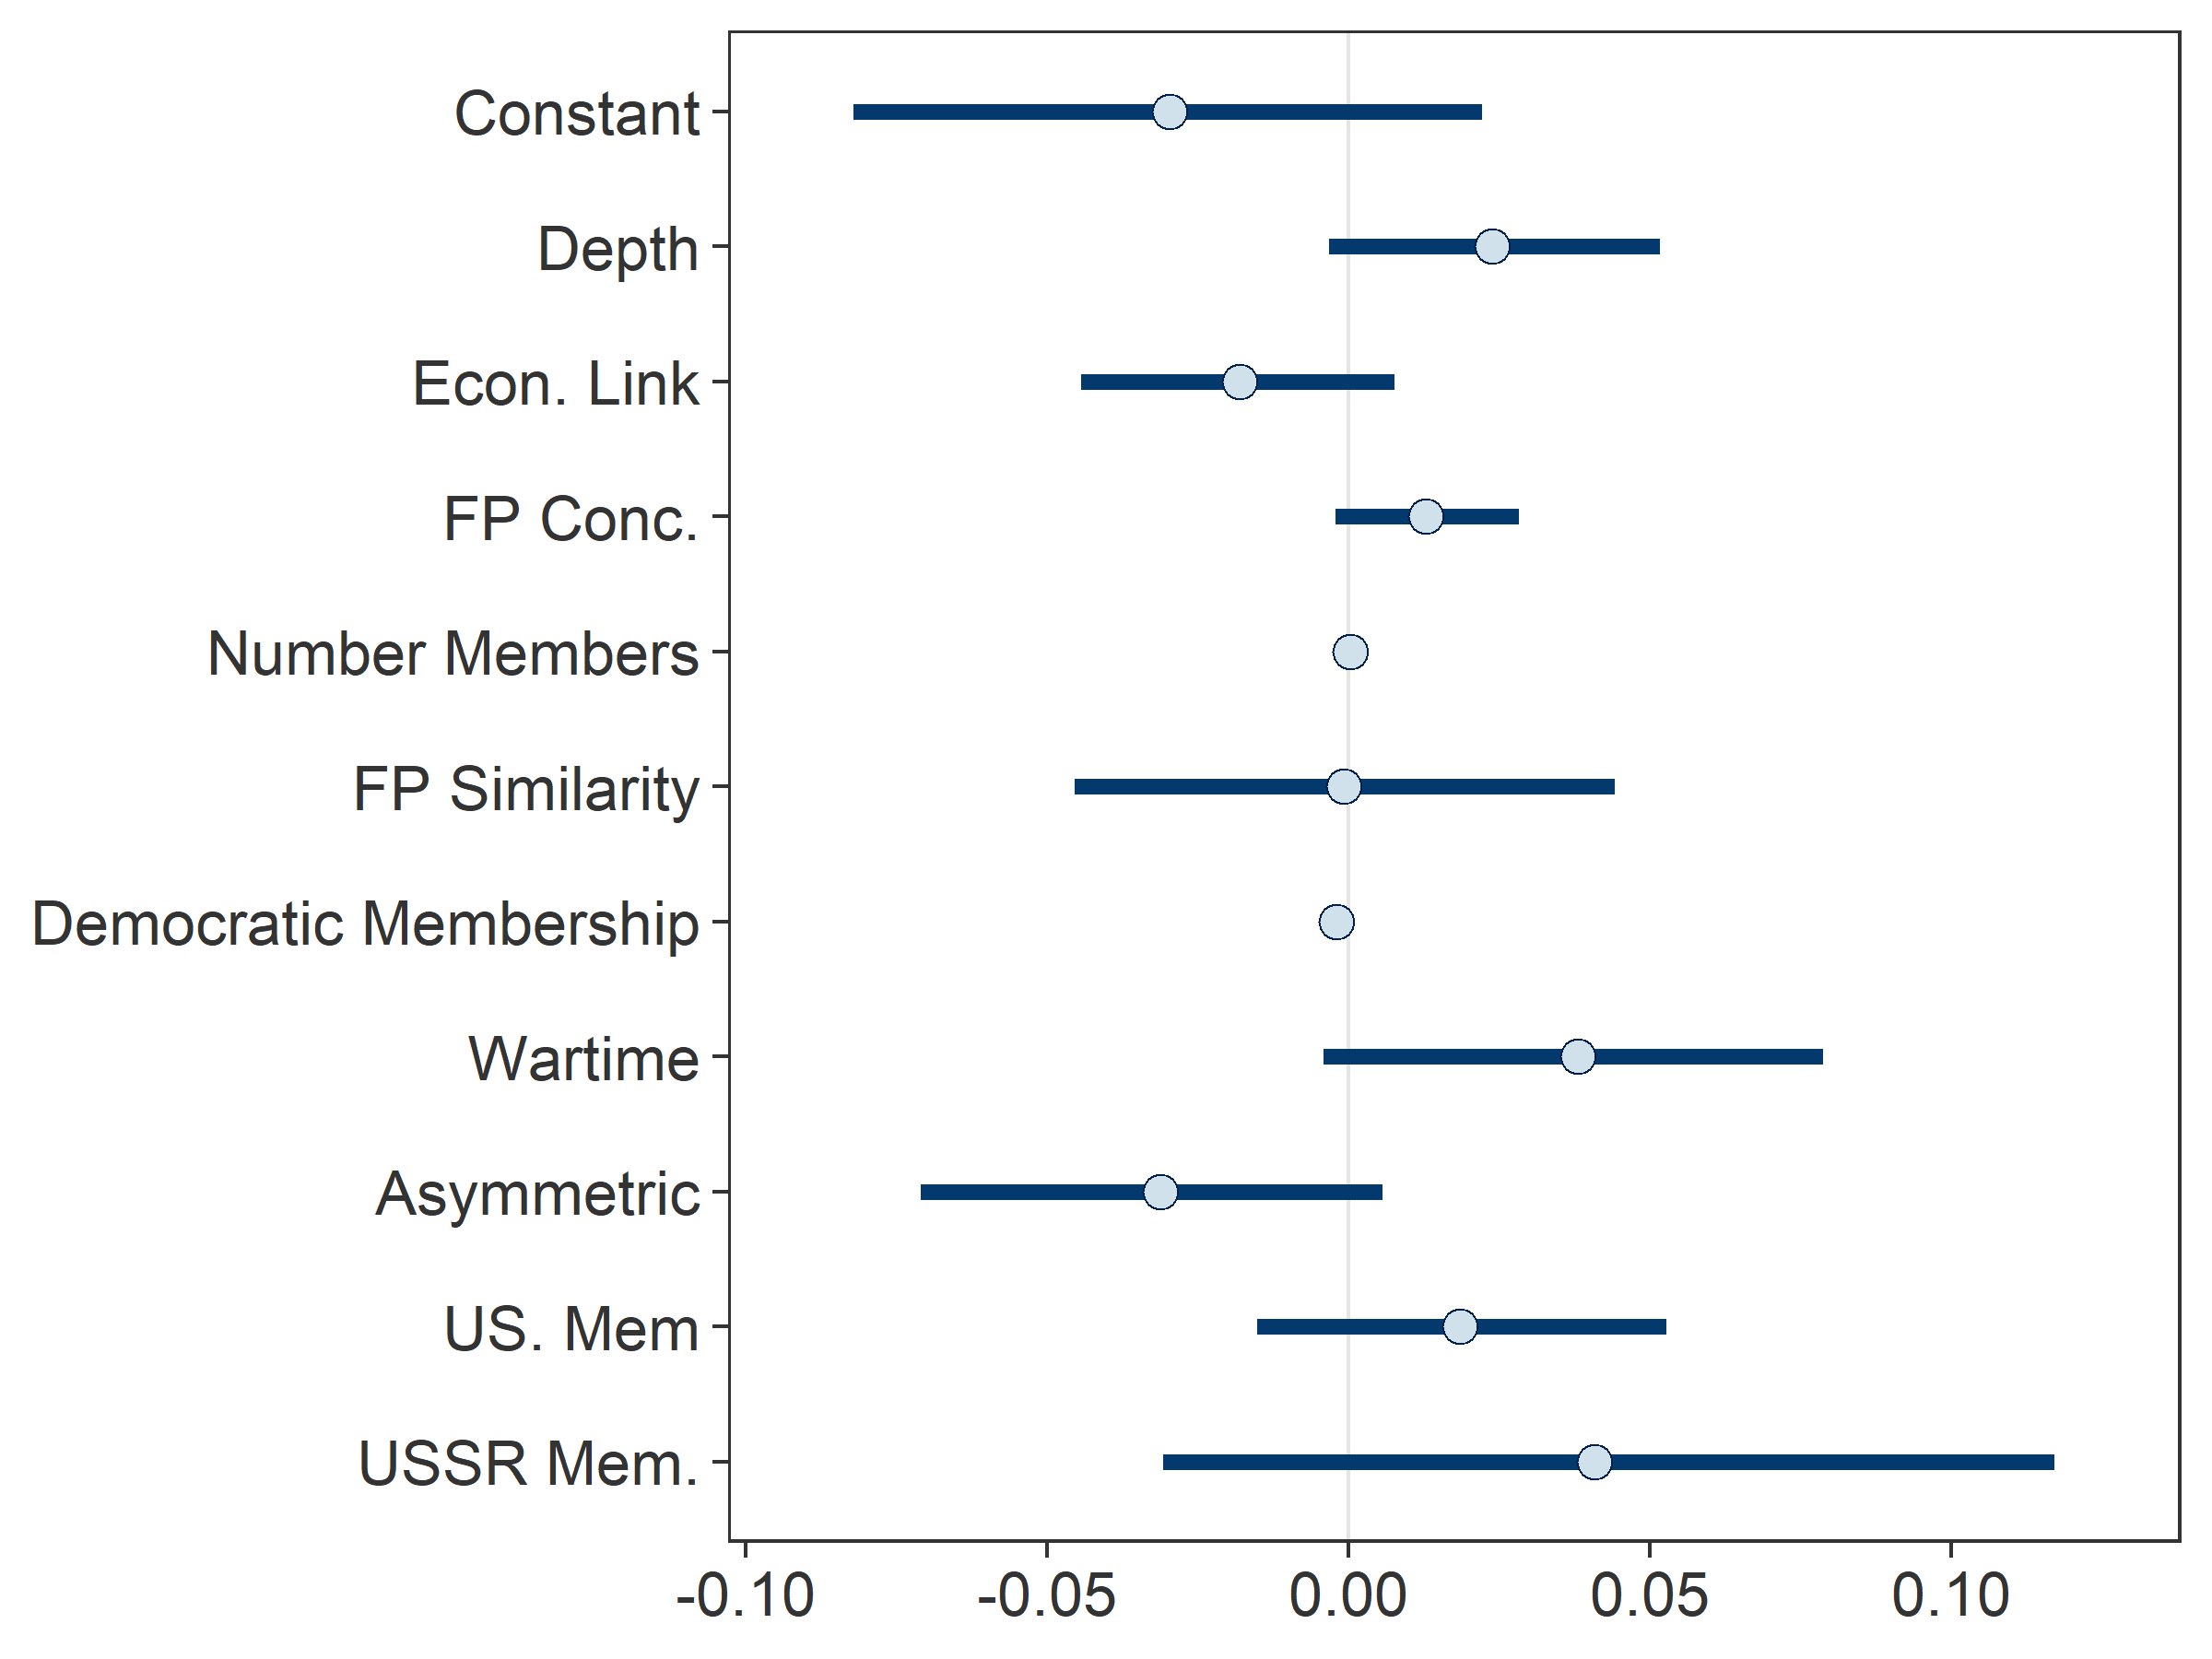
\includegraphics[width=0.9\textwidth]{beta-intervals-min.png}
	\label{fig:beta-intervals-min}
\end{figure}


\end{frame}

%------------------------------------------------

\section{US Alliances}

%------------------------------------------------

\begin{frame}{Foreign Entanglement and Shallow Formal Obligations}

\begin{figure}
	\centering
		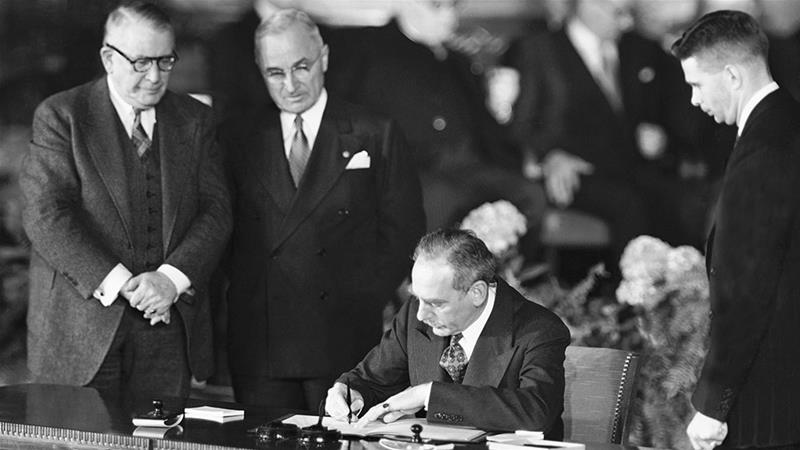
\includegraphics[width=0.95\textwidth]{acheson-nato-sign.jpg}
	\label{fig:acheson-nato-sign}
\end{figure}


\end{frame}

%------------------------------------------------

\begin{frame}[standout]

\large ``The Parties agree that an armed attack against one or more of them in Europe or North America shall be considered an attack against them all...'' 

 \end{frame}

%------------------------------------------------

\begin{frame}[standout]

\large ``assist the Party or Parties so attacked by taking forthwith, individually and in concert with the other Parties, such action as it deems necessary, including the use of armed force'' 

 \end{frame}

%------------------------------------------------

\begin{frame}[standout]

\huge ``such action as it deems necessary, including the use of armed force'' 

 \end{frame}

%------------------------------------------------

\begin{frame}{US Alliances in Context} 

\begin{figure}
	\centering
		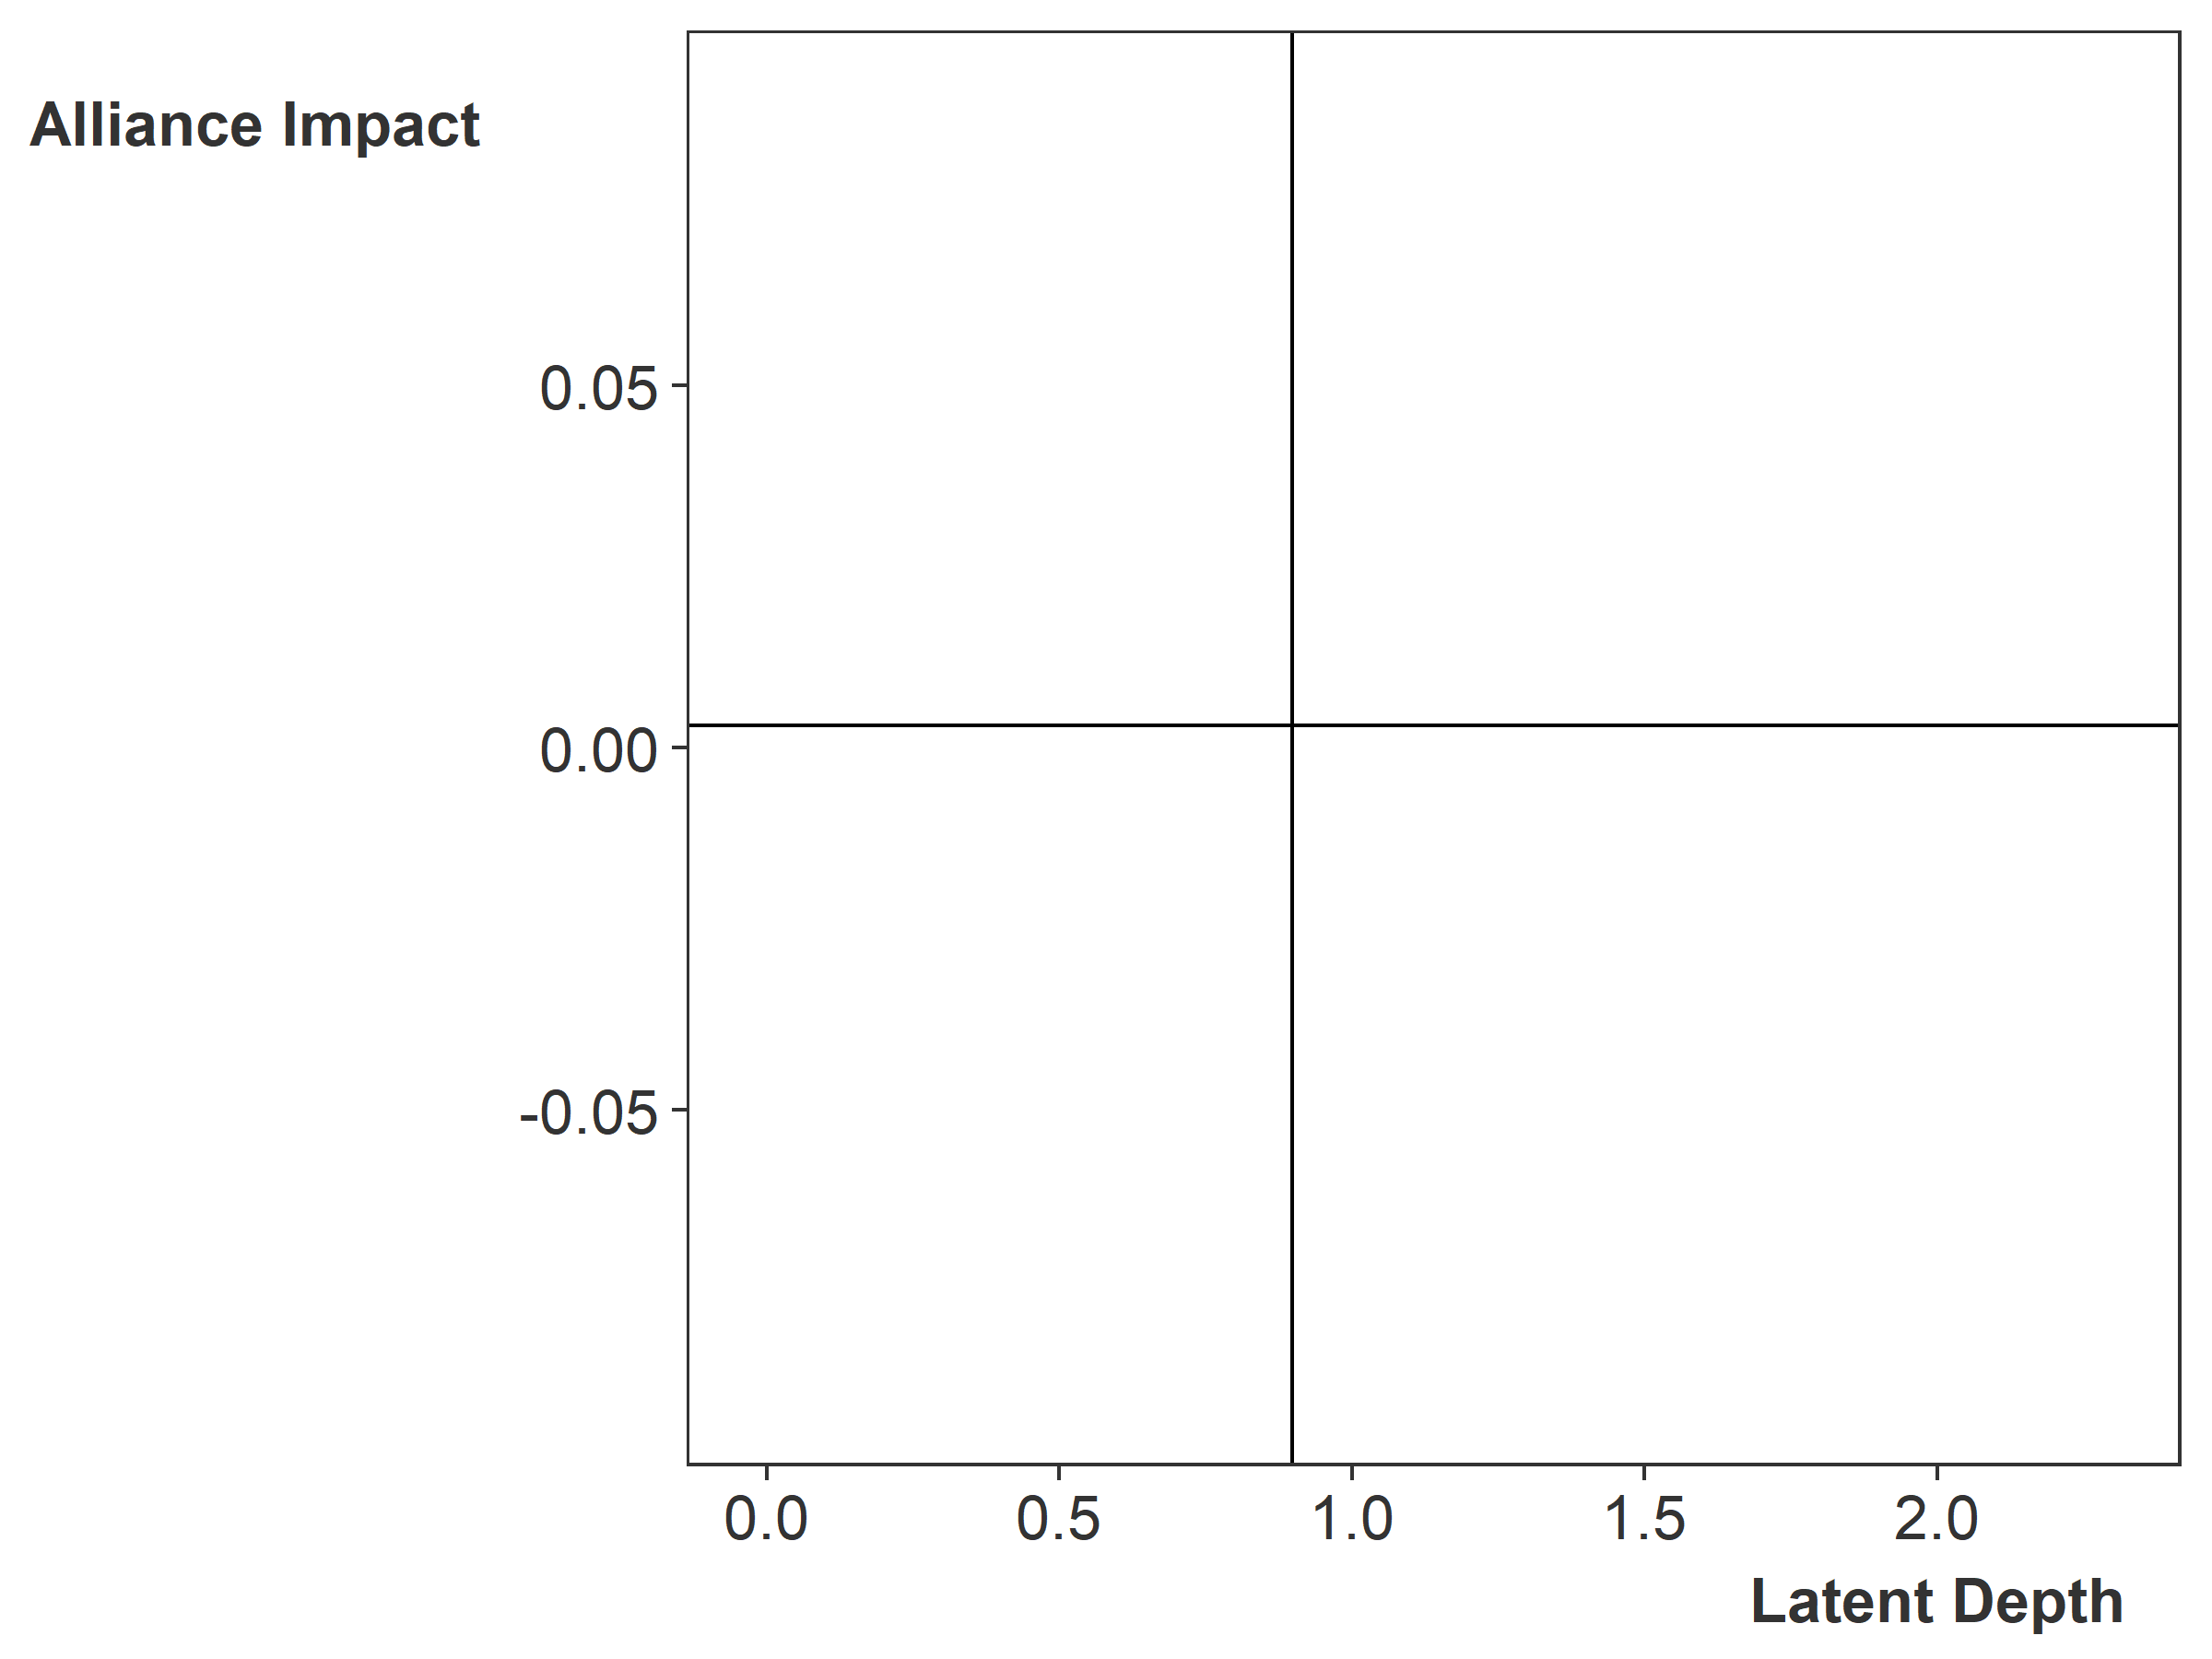
\includegraphics[width=0.95\textwidth]{lambda-depth-us-blank.png}
\end{figure}


 \end{frame}
 
 
%------------------------------------------------

\begin{frame}{US Alliances in Context} 

\begin{figure}
	\centering
		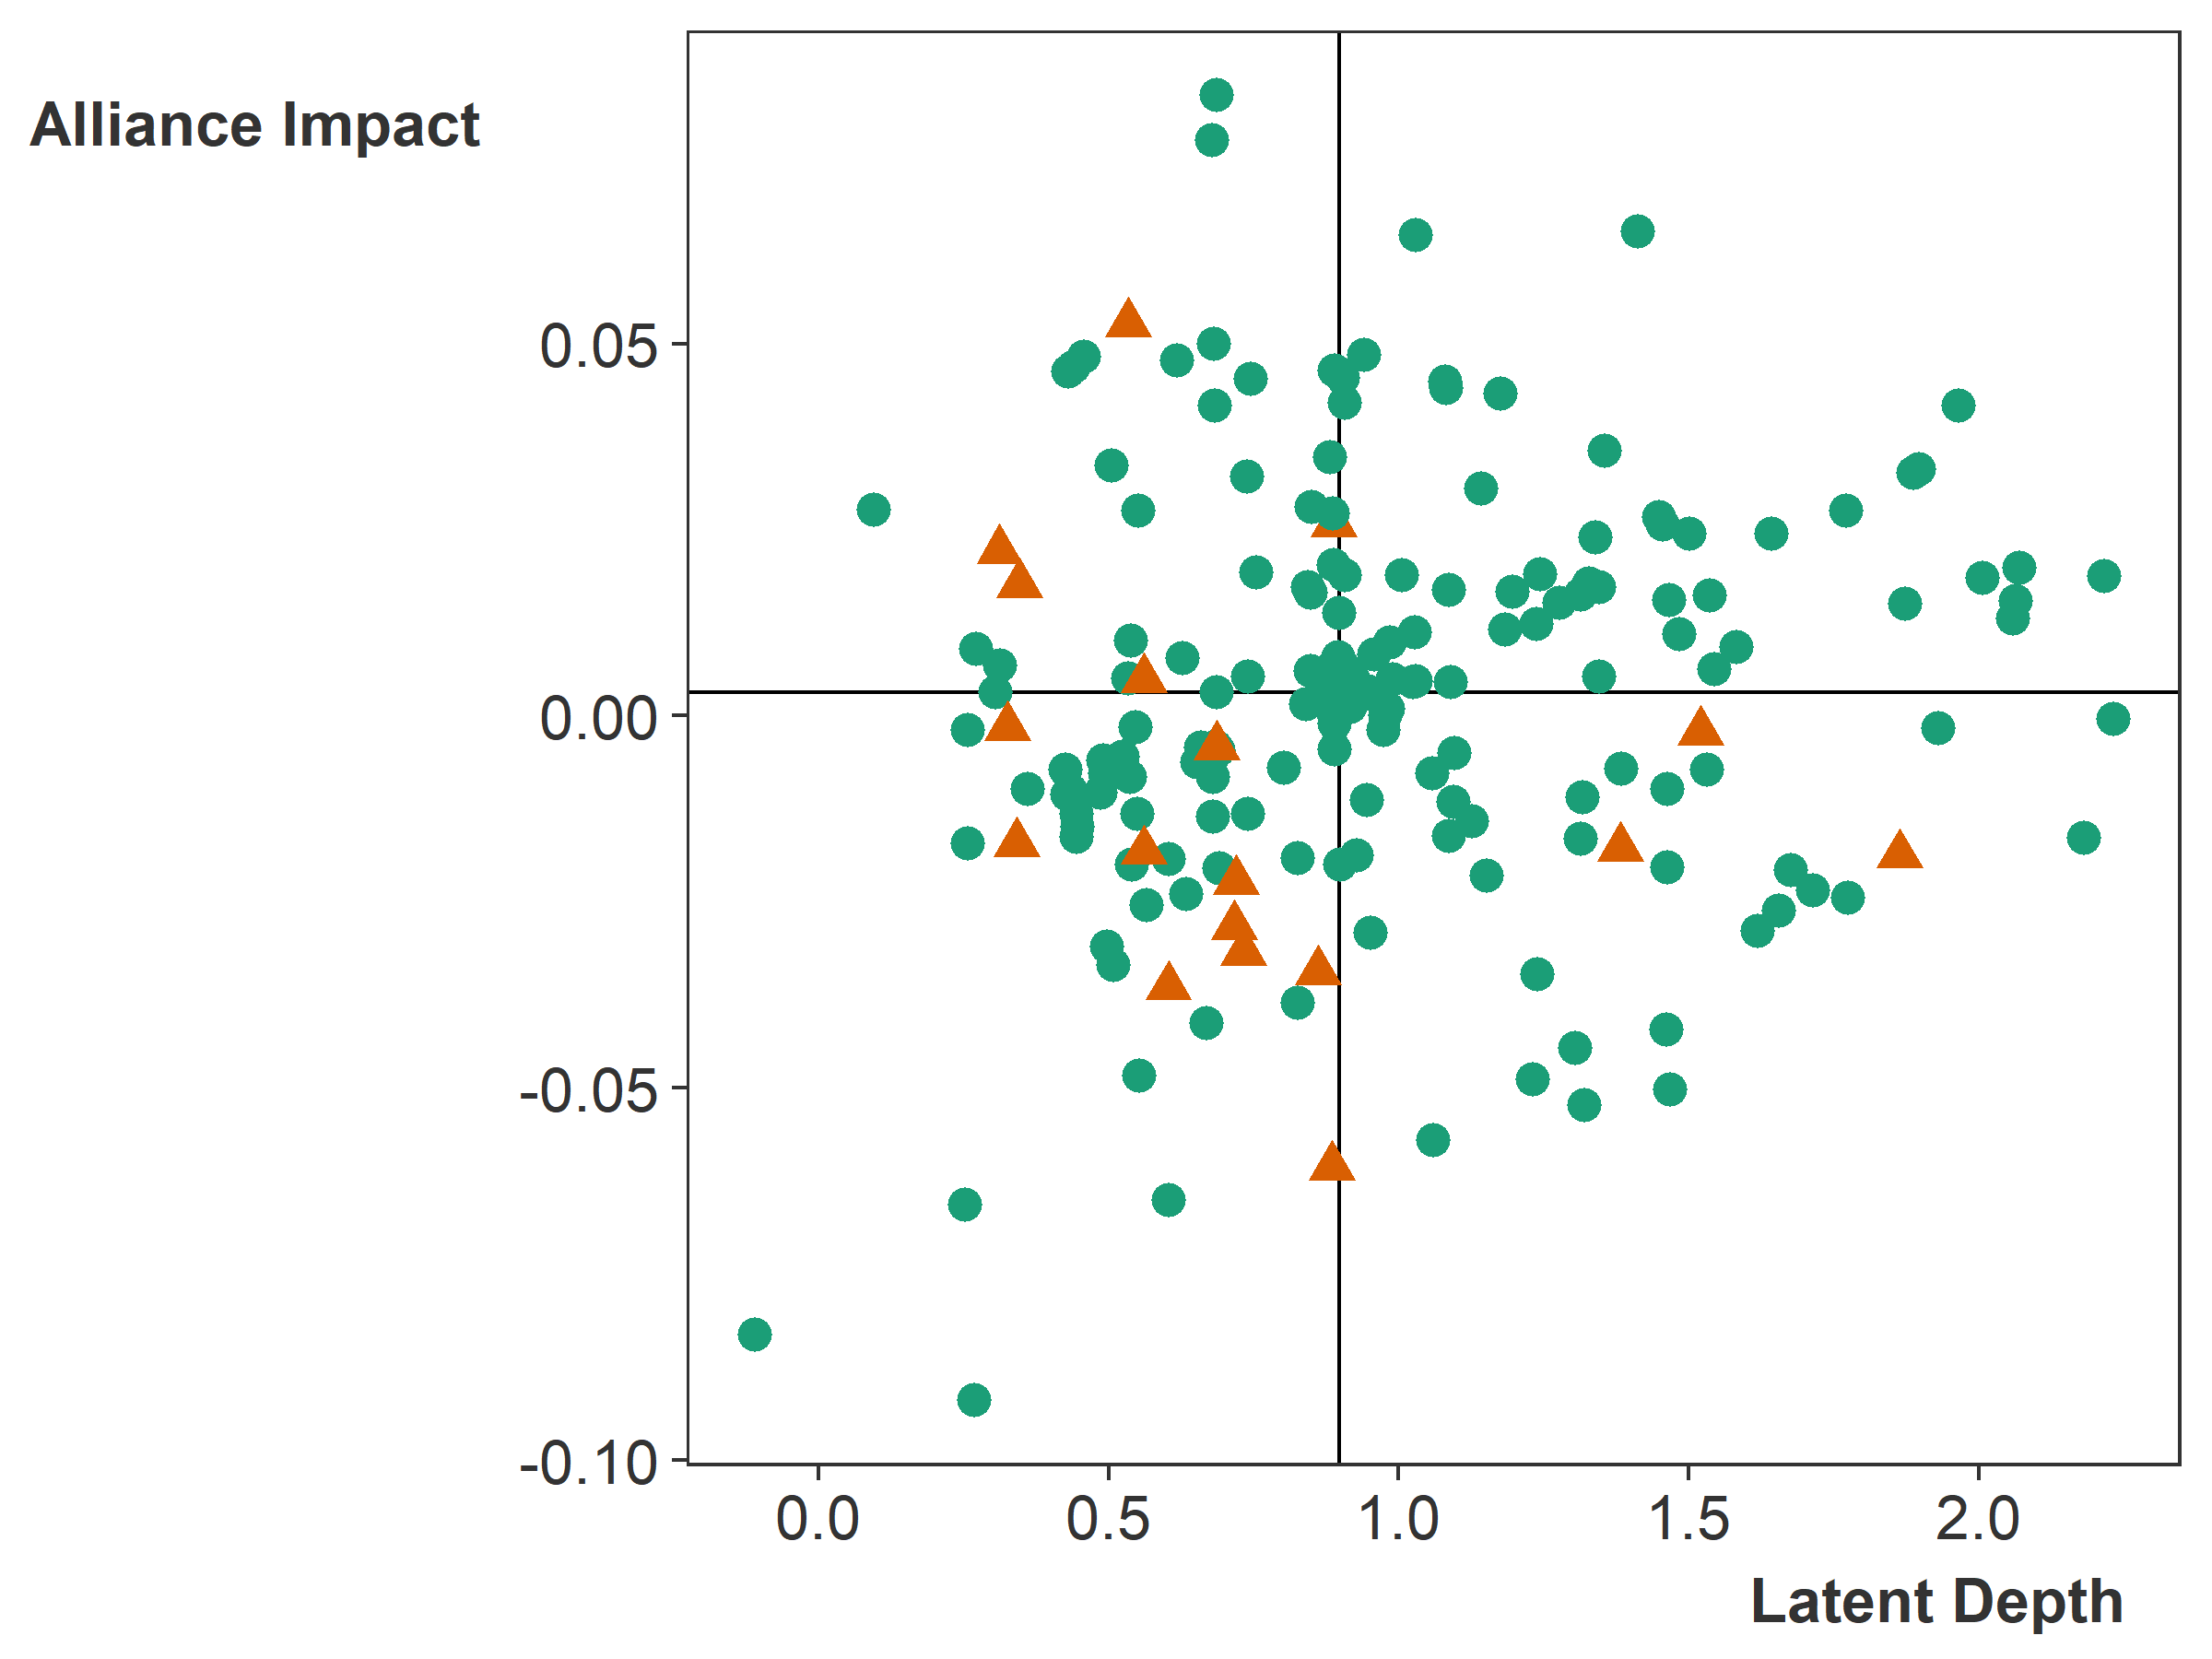
\includegraphics[width=0.95\textwidth]{lambda-depth-us.png}
\end{figure}


 \end{frame}



%-----------------------------------------------

\begin{frame}{Implication: What to do with US alliances?}

\begin{figure}[htbp]
	\centering
		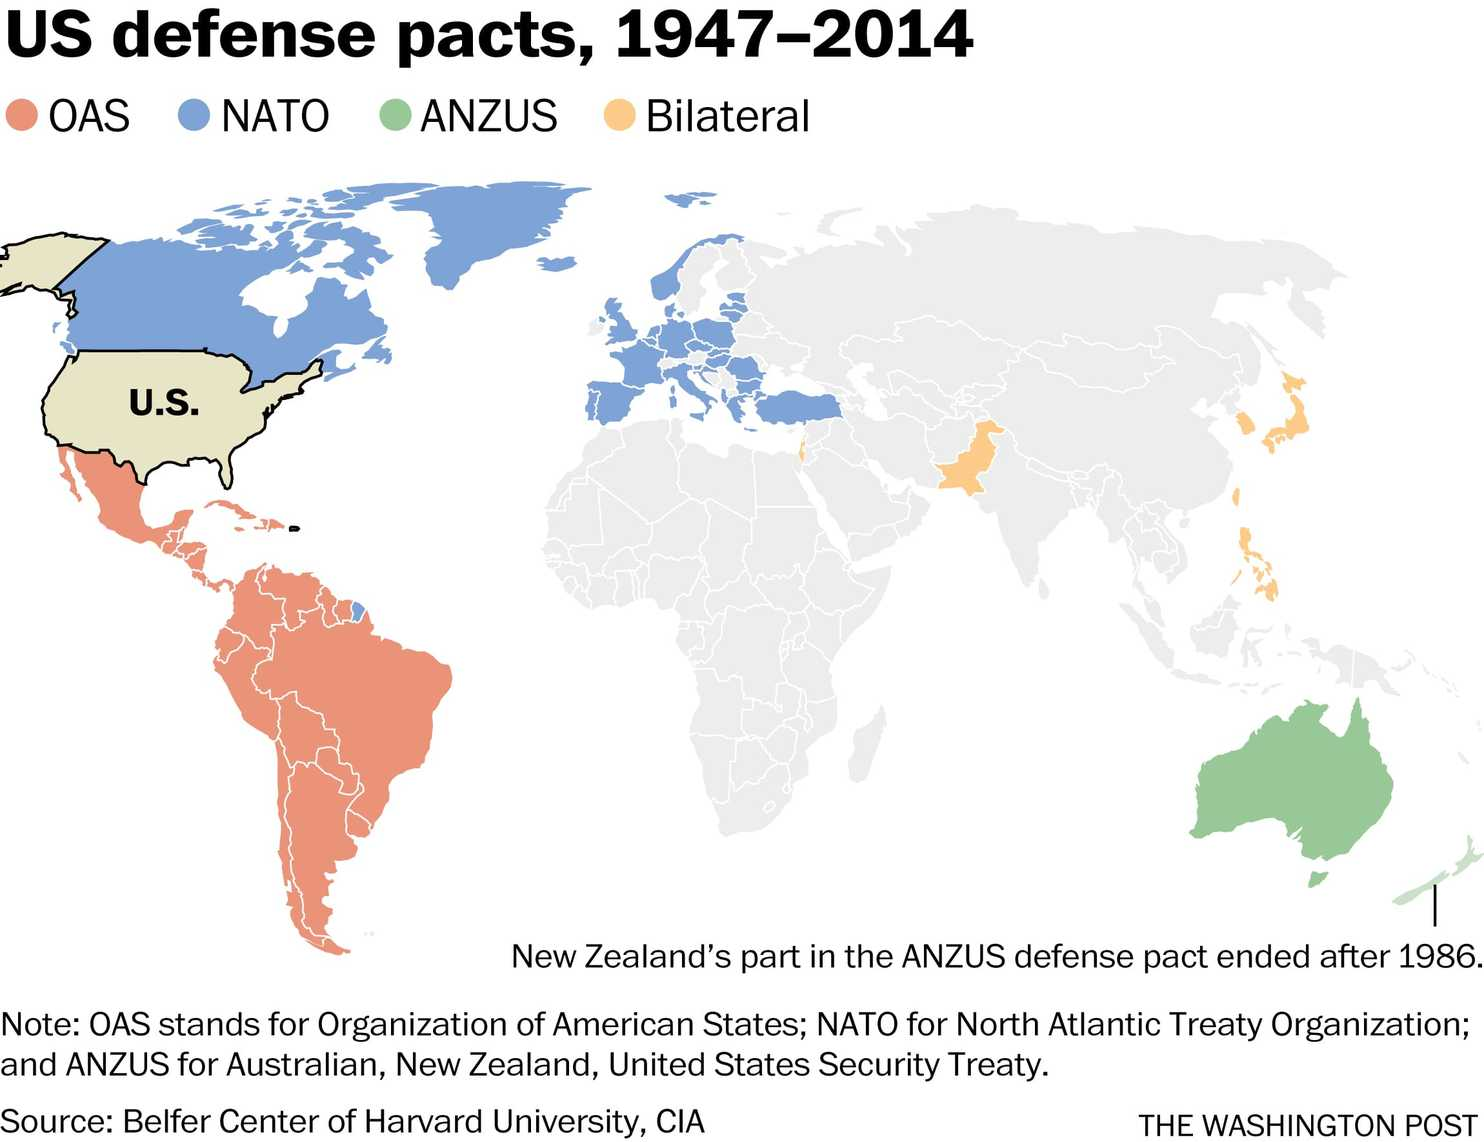
\includegraphics[width=0.95\textwidth]{nato-map.jpg}
\end{figure}


\end{frame}


%-----------------------------------------------

\section{Conclusion}

%-----------------------------------------------

\begin{frame}[standout]

How alliance participation affects military spending depends on treaty depth.  

\end{frame}

%------------------------------------------------
% The two subpoints 
 \begin{frame}[standout]

Though alliance participation usually decreases non-major power military spending, growth is higher in deep treaties.

 \end{frame}


%-----------------------------------------------

\section{Looking Ahead}

%-----------------------------------------------

\begin{frame}{Dissertation}

My dissertation articulates and tests a more general theory of alliance participation and military spending. 

\end{frame}


%-----------------------------------------------


\begin{frame}{My Research Agenda}

The political economy of security, with a focus on formal institutions. 

\begin{columns}

% Major powers
\begin{column}{0.5\textwidth}
\textbf{International Security}
\begin{itemize} 
\item Alliance Participation, Treaty Depth and Military Spending 
\item Reassessing the Public Goods Theory of Alliances
\end{itemize} 
\end{column}



\begin{column}{0.5\textwidth}
\textbf{Intra-State Conflict}
\begin{itemize}
\item Conflict Management Institutions and FDI
\item Sanctioning Terrorist Groups: Can it Work?
\item Weapon of the Weak?: Rebel Groups' International Law Talk, 1974-2011
\end{itemize} 
\end{column}

\end{columns}
 

\end{frame}


%-----------------------------------------------

 \begin{frame}[standout]

Thank you! 

jkalley14@tamu.edu

 \end{frame}


%-----------------------------------------------

\appendix 


%-----------------------------------------------

\begin{frame}{Limitations}

\begin{enumerate}
\item Domestic political economy of military spending. 
\item Measurement error and missing data. 
\item Formal depth only in the measure. 
\item Strategic alliance design
\end{enumerate}

\end{frame}


%-----------------------------------------------

\begin{frame}{Spending Growth and the Hypotheses}

\begin{figure}
	\centering
		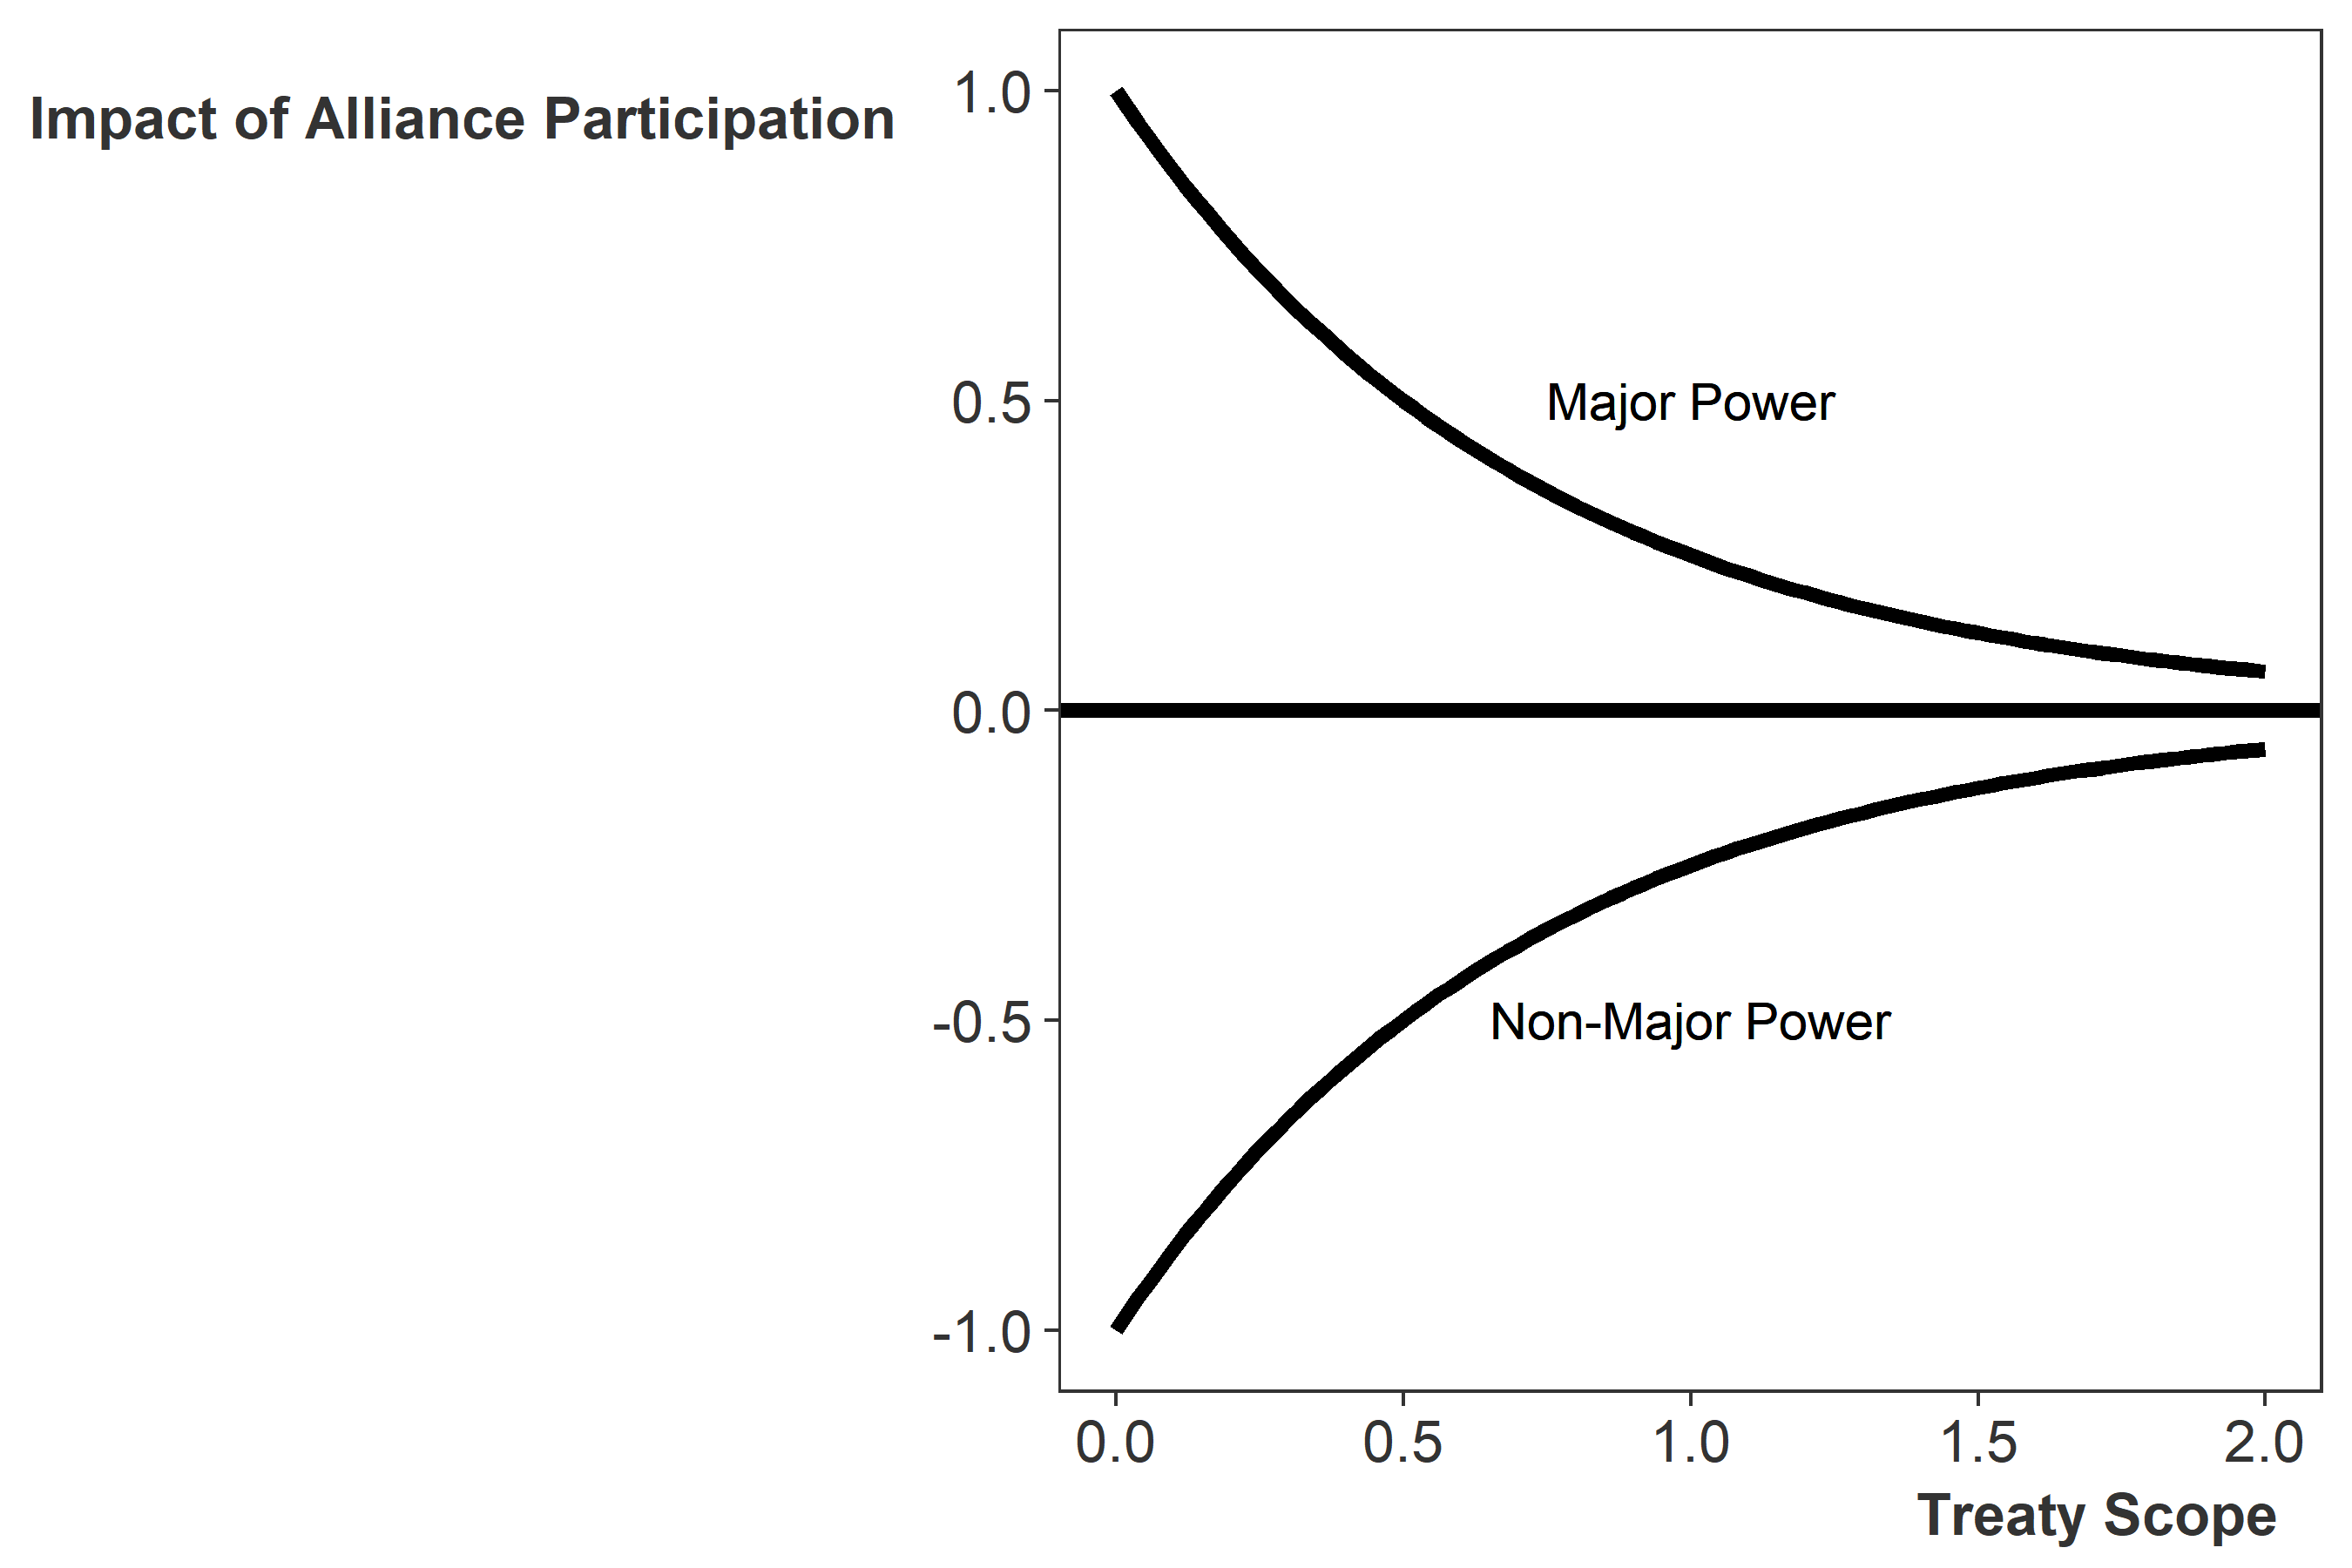
\includegraphics[width=0.95\textwidth]{illus-arg.png}
	\label{fig:illus-arg}
\end{figure}


\end{frame}


%-----------------------------------------------

\begin{frame}{Trace plots: Non-Major}

\begin{figure}
	\centering
		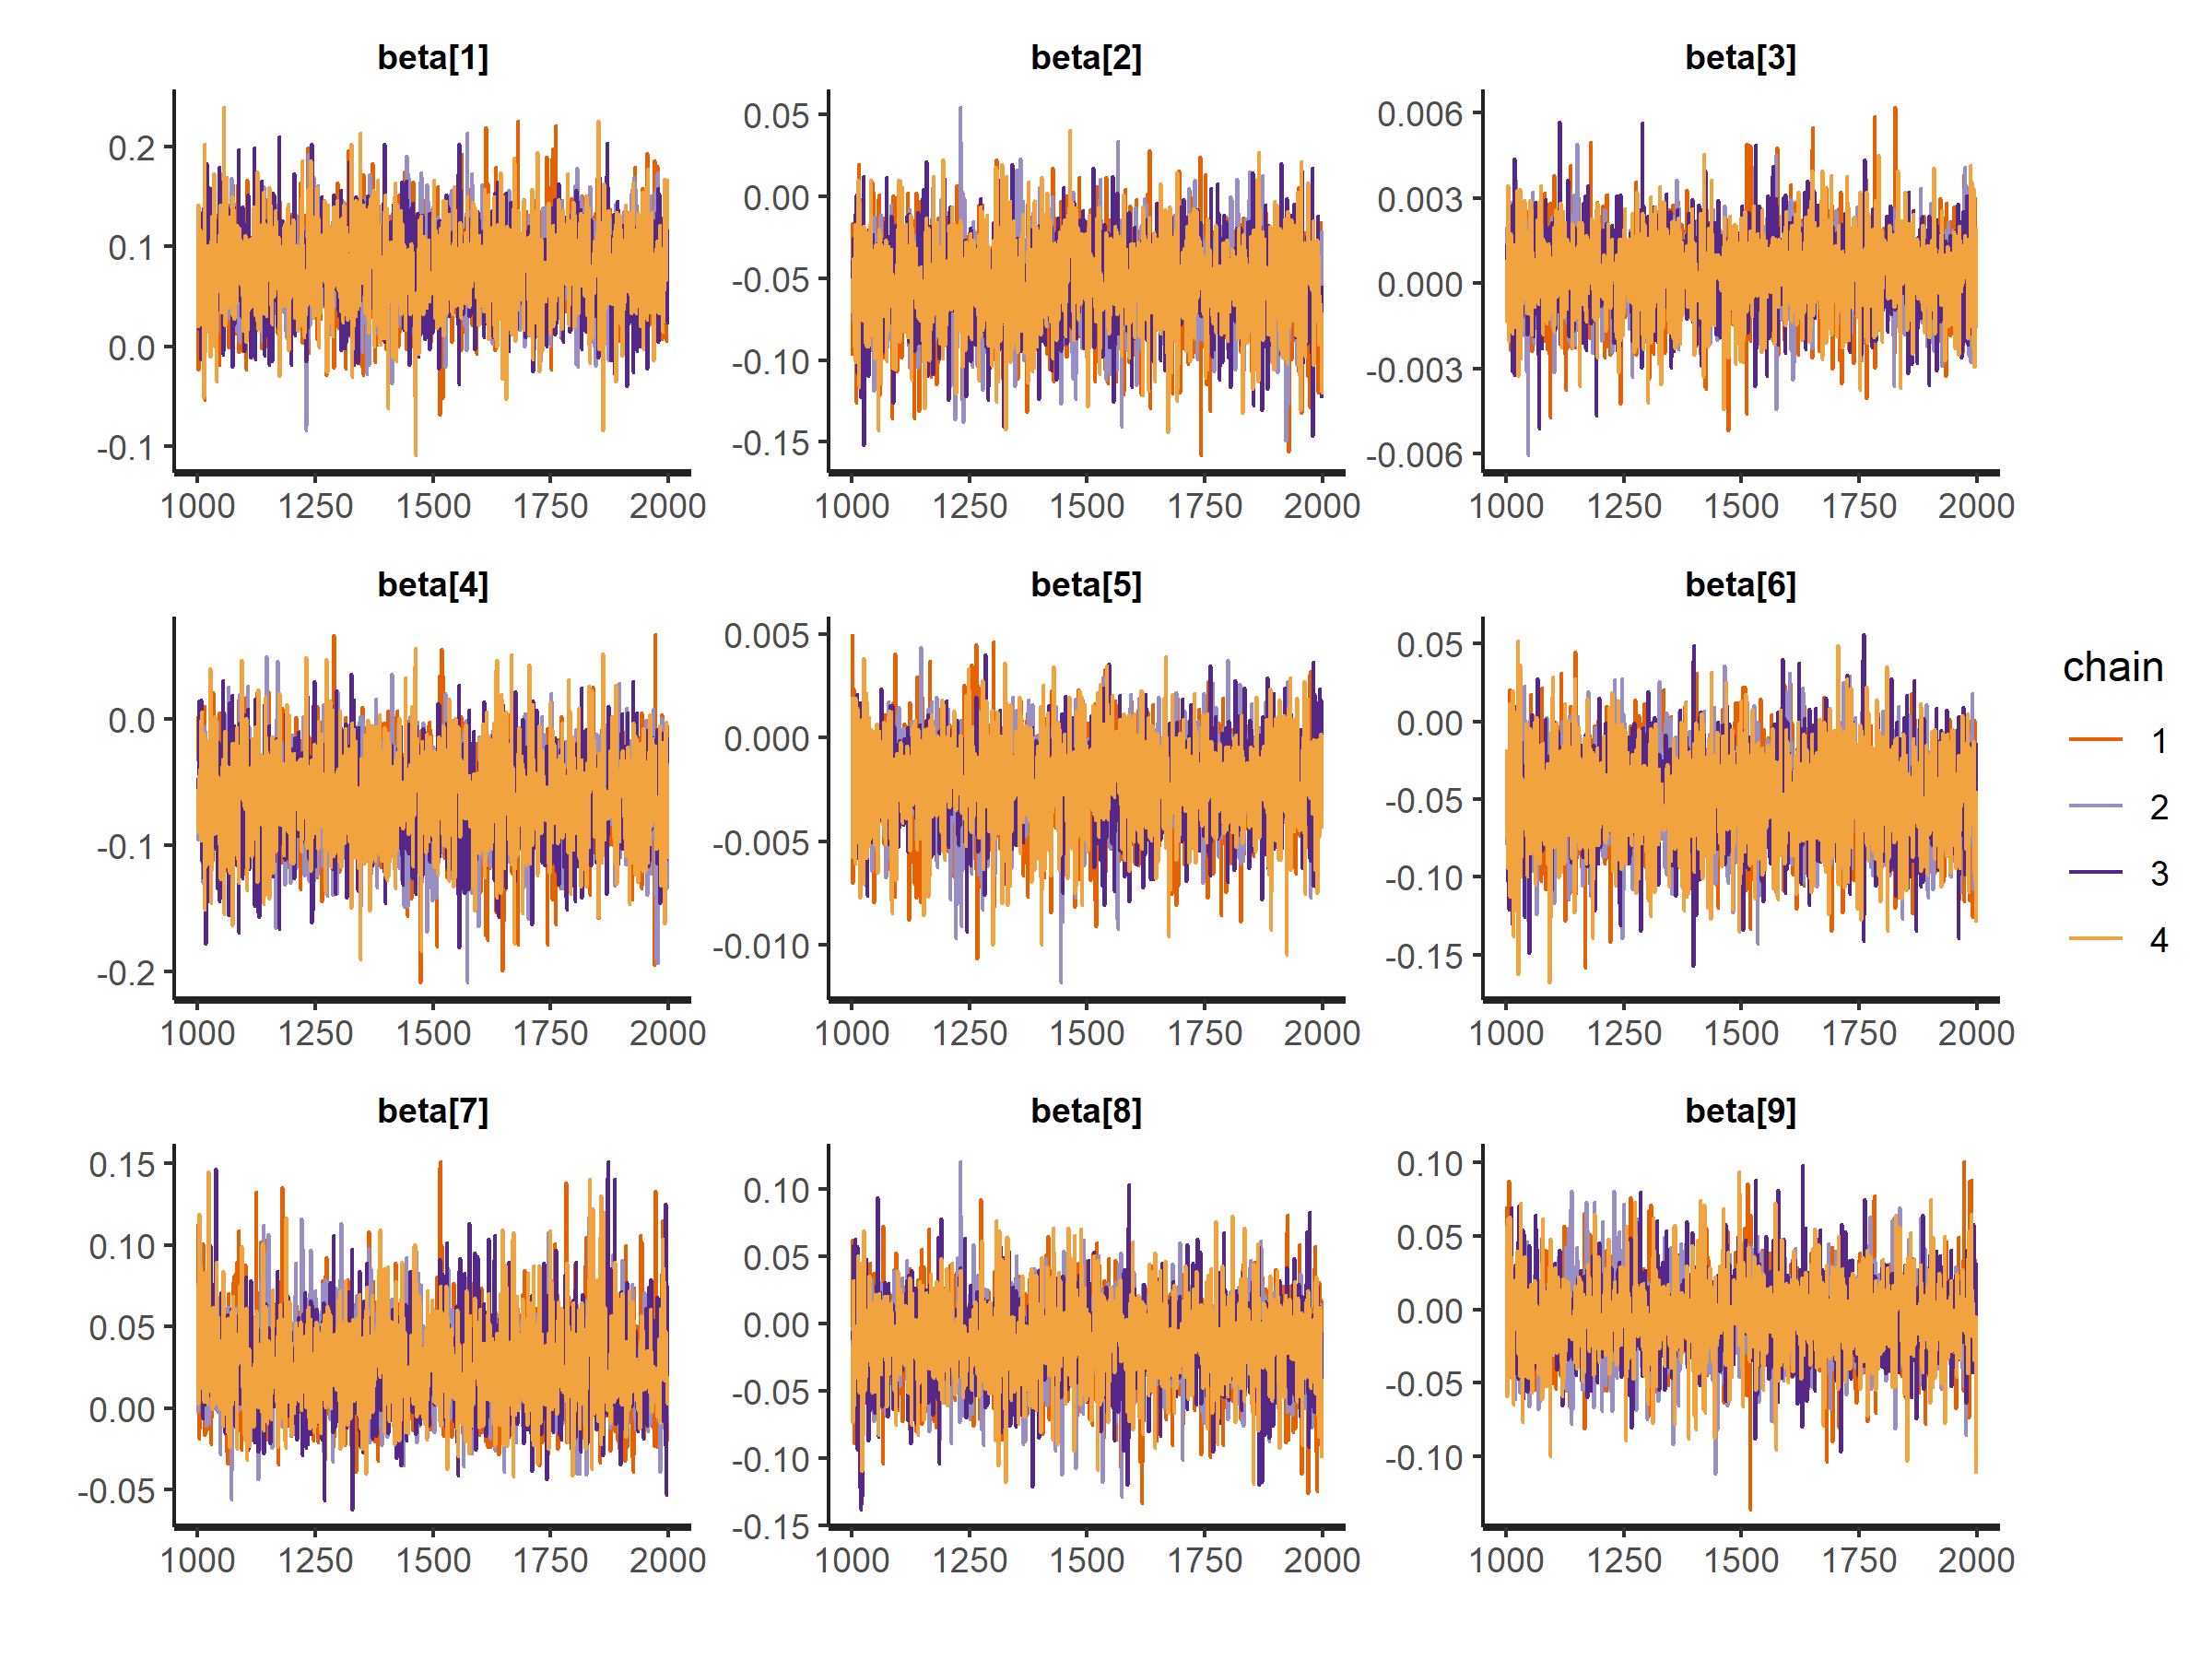
\includegraphics[width=0.95\textwidth]{beta-trace-maj.png}
\end{figure}


\end{frame}


%-----------------------------------------------

\begin{frame}{Model Check: Recovering Known Parameters}

Another way to check complicated models is simulating fake data with known parameters, then using the model to recover said parameters. 

To check my model, I simulated a fake dataset of 2,000 observations with 50 states, 200 years, 100 alliances and 2 variables at each level.

The 90\% credible intervals contain the known value for all regression parameters. 93 of 100 alliance specific parameter intervals contain the known value. 

\end{frame}


%-----------------------------------------------

\begin{frame}{Simulated Parameters and Credible Intervals}


\begin{figure}
	\centering
		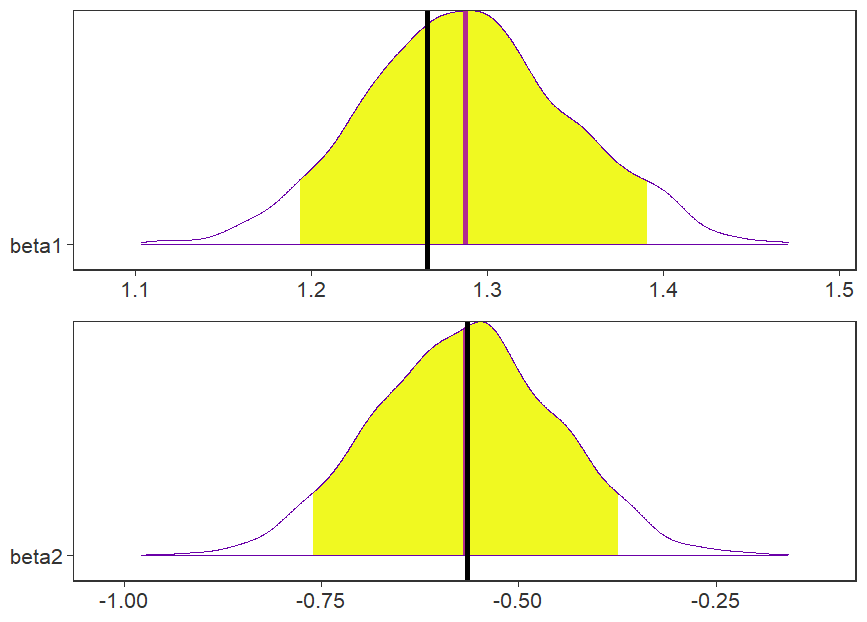
\includegraphics[width=0.95\textwidth]{sim-check-res.png}
\end{figure} 

\end{frame}



%-----------------------------------------------

\begin{frame}{Alliance-Level Regression Table: Non-Major Powers}

8,668 observations and 192 alliances. 

\resizebox{.95\textwidth}{!}{
\begin{tabular}{rrrrrrr}
  \hline
 & mean & sd & 5\% & 95\% & n\_eff & $\hat{R}$ \\ 
  \hline
Constant & -0.03 & 0.03 & -0.08 & 0.02 & 1677.92 & 1.00 \\ 
  Depth & 0.02 & 0.02 & -0.00 & 0.05 & 2521.36 & 1.00 \\ 
  Econ. Link & -0.02 & 0.02 & -0.04 & 0.01 & 2997.70 & 1.00 \\ 
  FP Conc. & 0.01 & 0.01 & -0.00 & 0.03 & 4019.10 & 1.00 \\ 
  Number Members & 0.00 & 0.00 & -0.00 & 0.00 & 3820.06 & 1.00 \\ 
  FP Similarity & 0.00 & 0.03 & -0.04 & 0.05 & 2254.34 & 1.00 \\ 
  Democratic Membership & -0.00 & 0.00 & -0.00 & 0.00 & 4412.89 & 1.00 \\ 
  Wartime & 0.04 & 0.03 & -0.01 & 0.08 & 3474.44 & 1.00 \\ 
  Asymmetric & -0.03 & 0.02 & -0.07 & 0.01 & 3474.45 & 1.00 \\ 
  US. Mem & 0.02 & 0.02 & -0.01 & 0.05 & 2330.47 & 1.00 \\ 
  USSR Mem. & 0.04 & 0.05 & -0.03 & 0.12 & 3859.50 & 1.00 \\ 
  $\sigma$ Alliances & 0.02 & 0.01 & 0.00 & 0.03 & 1201.91 & 1.01 \\ 
   \hline
\end{tabular}
}



\end{frame}


%------------------------------------------------


\begin{frame}{Priors}

4 Chains with 2,000 samples and 1,000 warmup iterations. 

\begin{table} % Create a table of priors.

 \begin{center}
\begin{tabular}{c} 
$ p(\alpha) \sim N(0, 1)$  \\
$ p(\sigma) \sim \mbox{half-}N(0, 1) $ \\
$ p(\alpha^{yr}) \sim N(0, \sigma^{yr}) $ \\ 
$ p(\sigma^{yr}) \sim N(0, 1) $ \\
$ p(\alpha^{st}) \sim N(0, \sigma^{st}) $ \\ 
$ p(\sigma^{st}) \sim \mbox{half-}N(0, .5) $ \\ 
$ p(\sigma^{all}) \sim \mbox{half-}N(0, .5) $ \\
$ p(\beta) \sim N(0, .5) $ \\
$ p(\gamma) \sim N(0, .5) $ \\ 
$ p(\nu) \sim gamma(2, 0.1)$ 
\end{tabular} 
\end{center} 
\label{tab:priors}
\end{table} 


\end{frame}


%------------------------------------------------

\begin{frame}{Details of Measurement Model}

\begin{itemize}
\item Bayesian Gaussian Copula Factor Model: for mixed data. 
\item Uses copulas to break dependence between latent factors and marginal distributions. 
\item Treats marginals as unknown and keeps them free of dependence. 
\item IMH proposal, 10,000 iteration warmup, 20,000 samples, thinned every 20 draws. 
\item Generalized double Pareto prior for the factor loading--- flexible generalized Laplace distribution with a spike at zero and heavy tails. 
\end{itemize} 


\end{frame}


%------------------------------------------------


\begin{frame}{Aside: Benson and Clinton 2016}

\begin{itemize}
\item Use a measurement model to infer alliance scope, depth and capability. 
\item Identify three separate dimensions, and use three models- explicit constraint. 
\item I use a different concept, which combines what they call scope and depth. 
\item Murray et al's model relaxes distributional assumptions in their estimator (Quinn 2004 Factor Analysis). 
\end{itemize}


\end{frame}

%------------------------------------------------

\begin{frame}{Latent Measure for all ATOP Alliances}


\begin{figure}
	\centering
		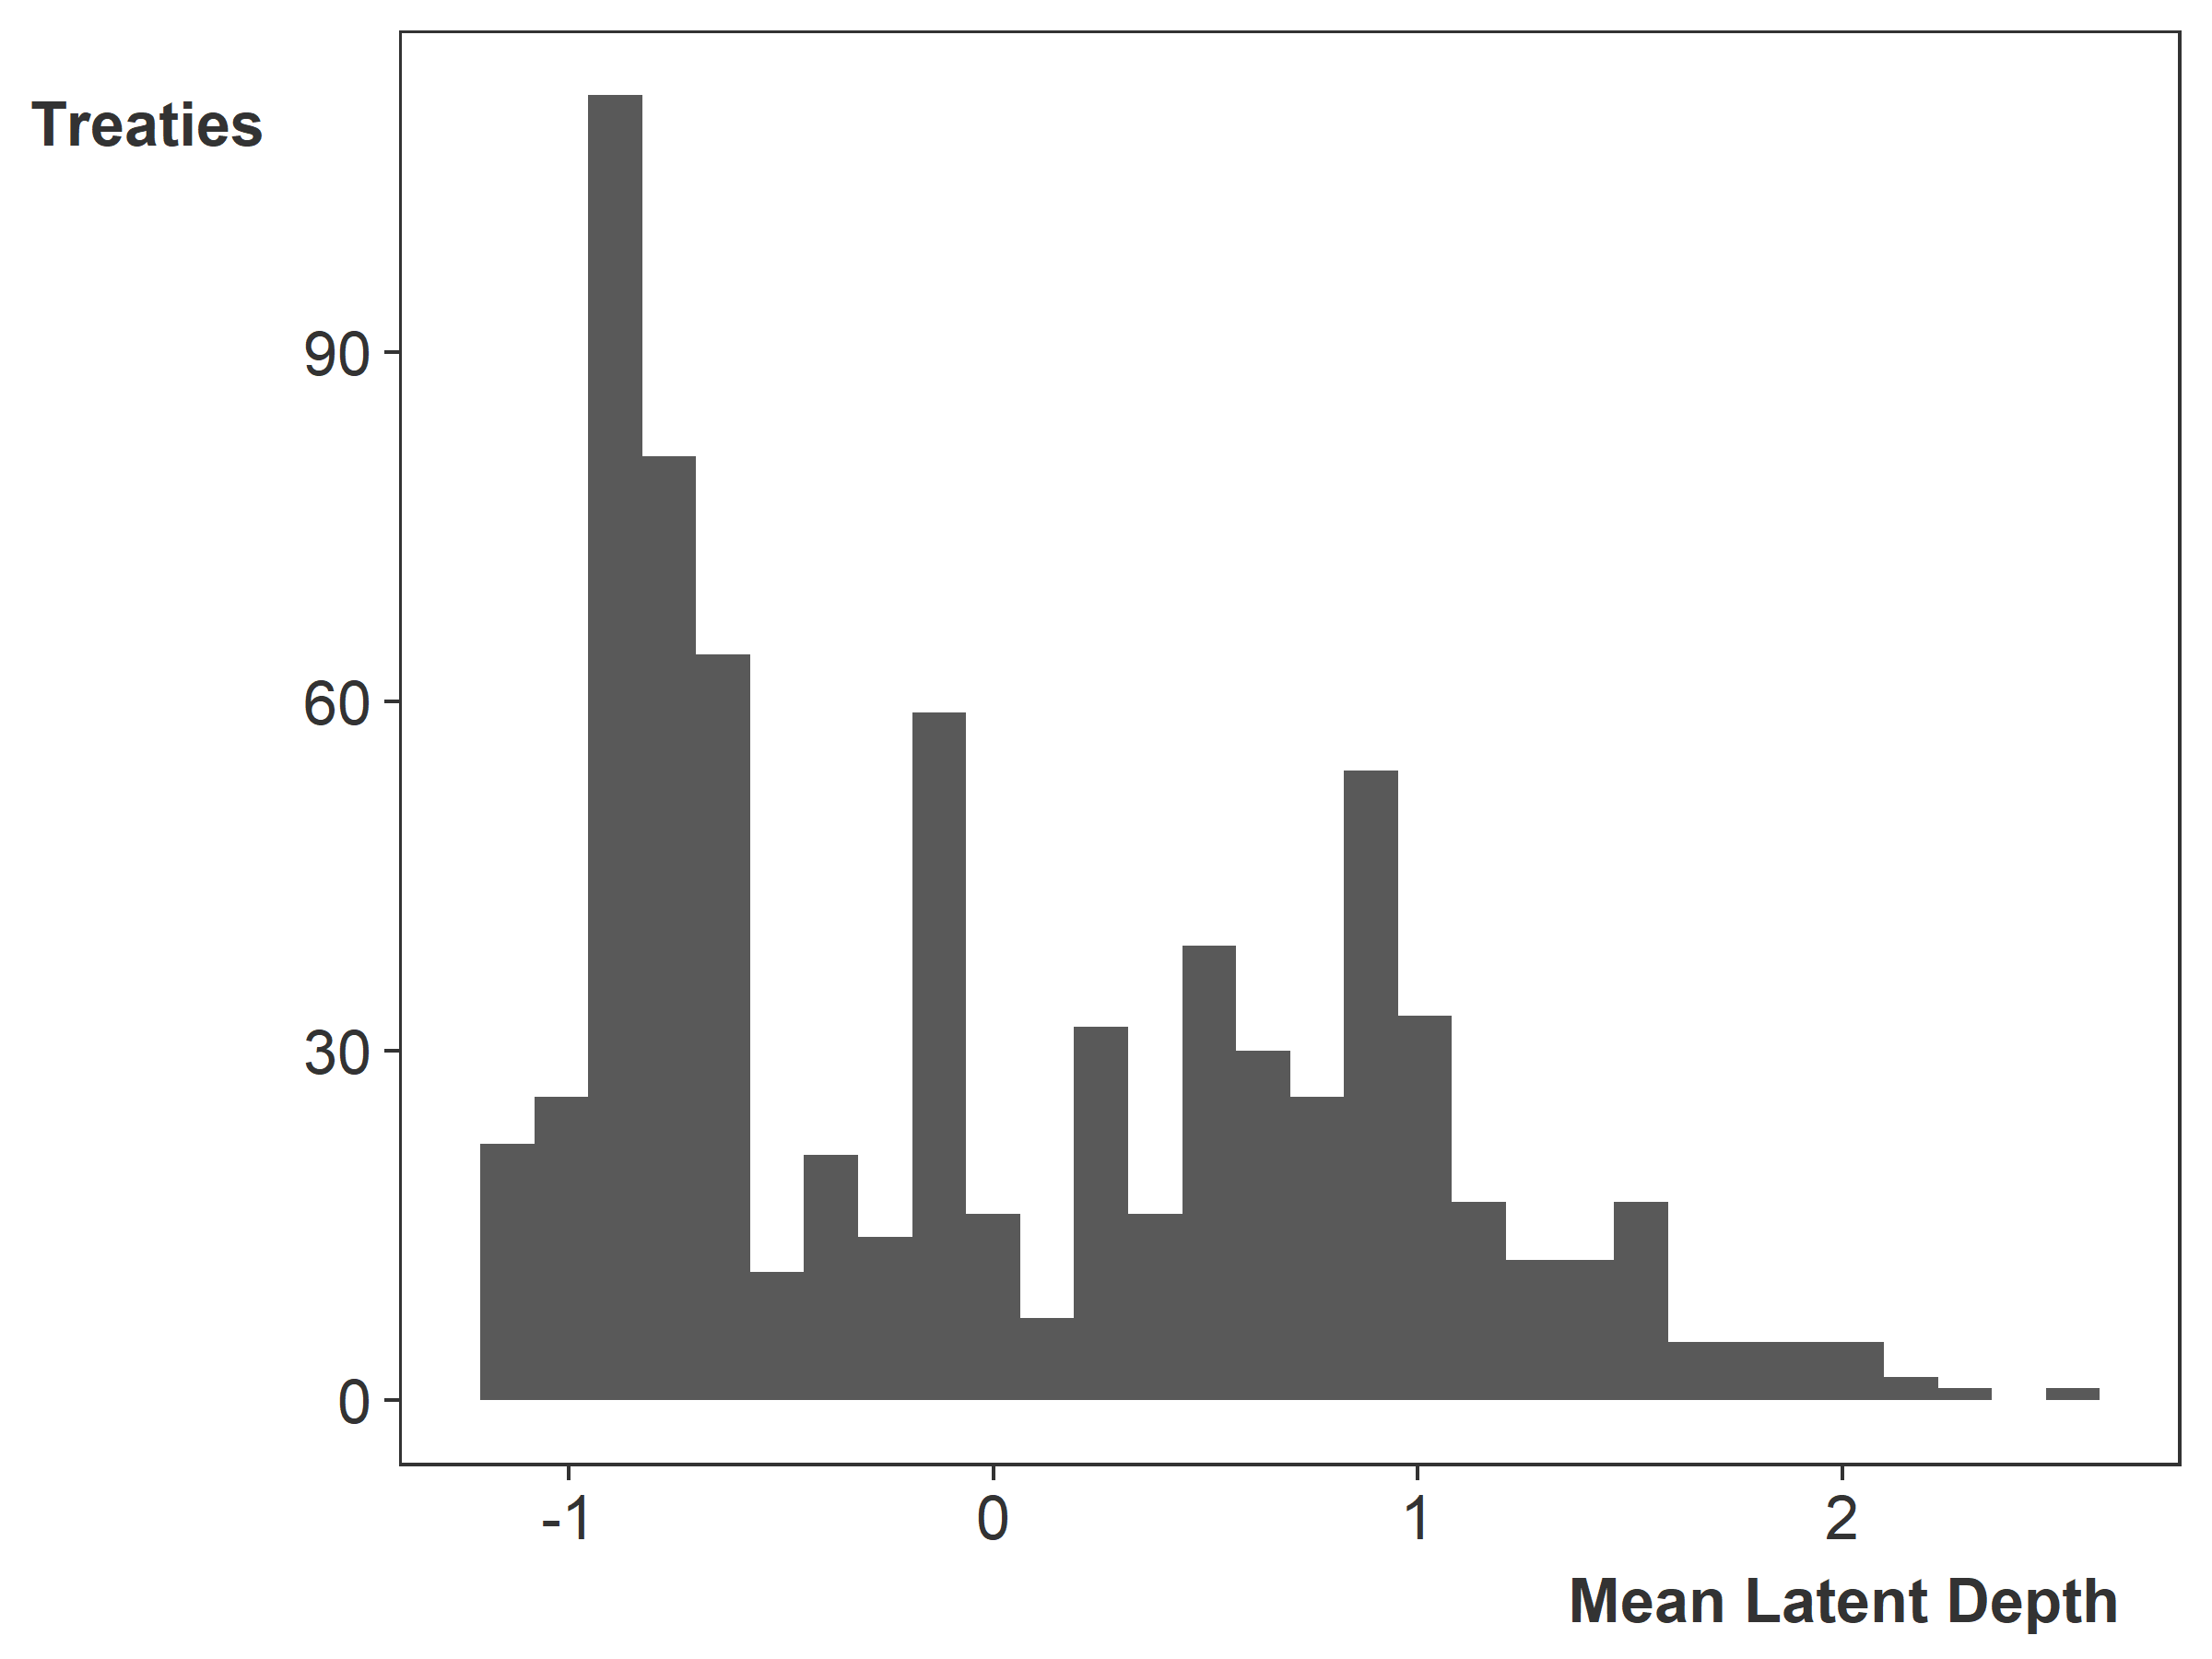
\includegraphics[width=0.95\textwidth]{ld-hist-full.png}
\end{figure}


\end{frame}


%------------------------------------------------

\begin{frame}{Factor Loadings}


\begin{figure}
	\centering
		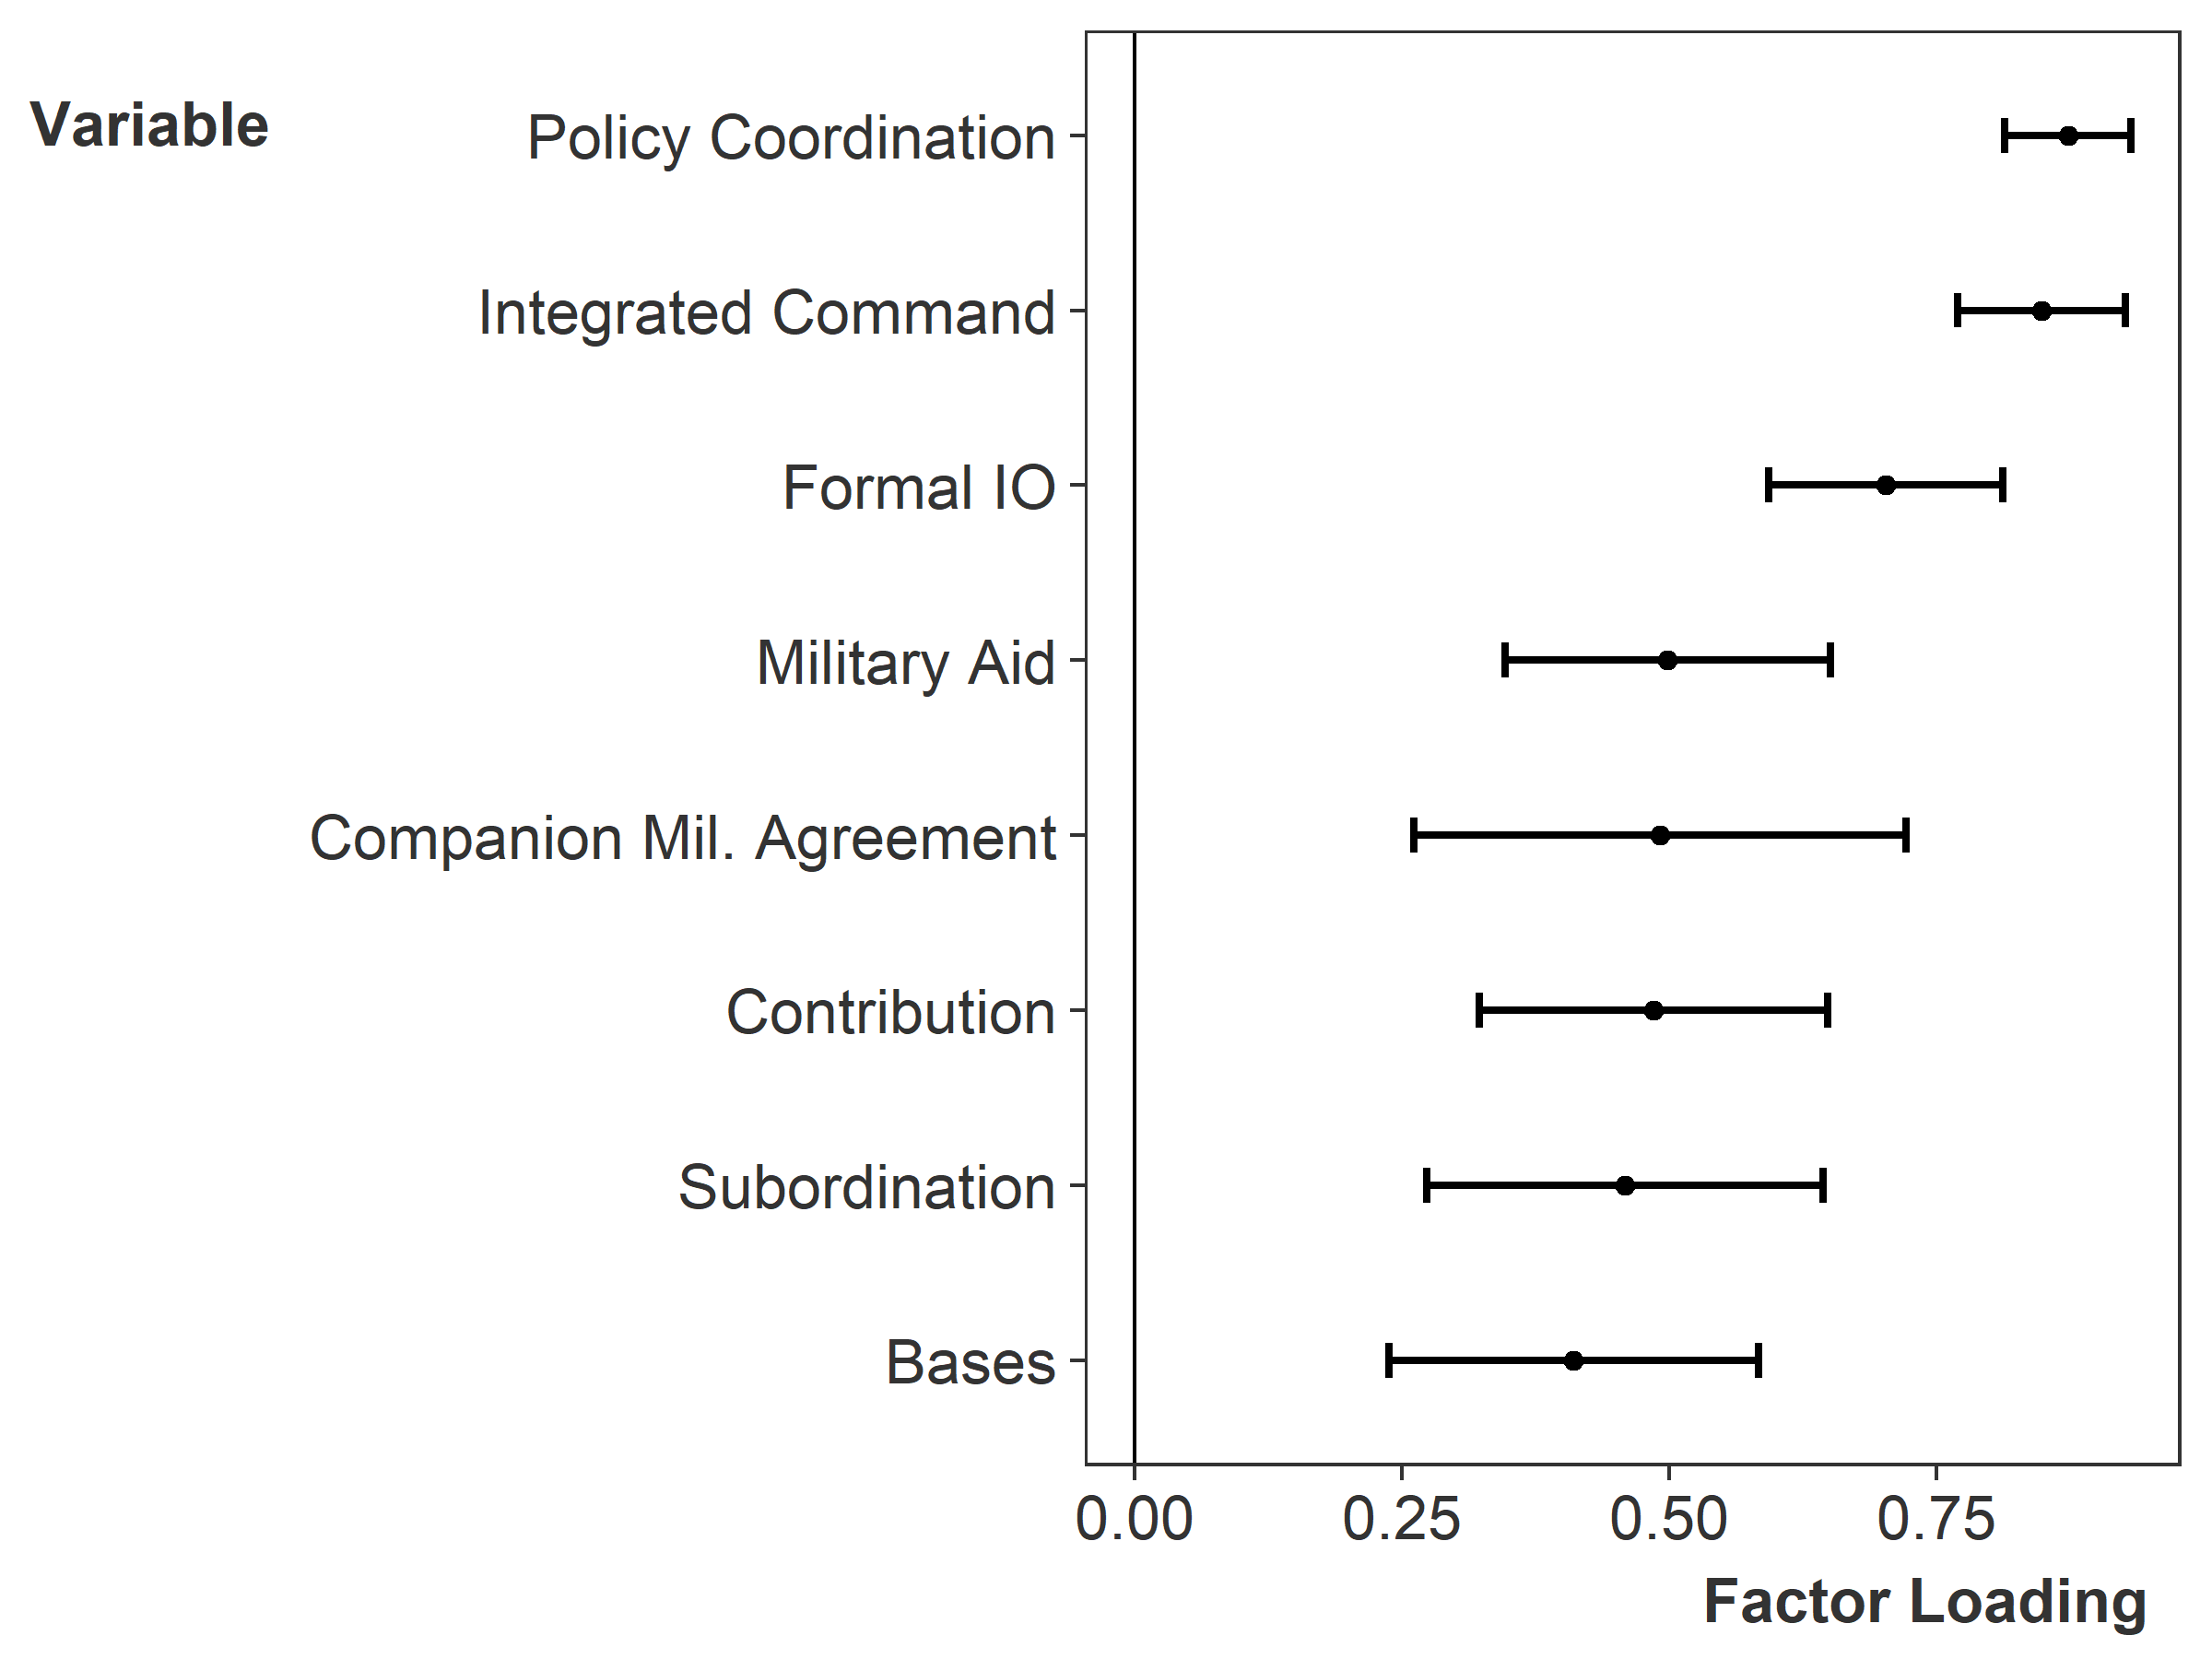
\includegraphics[width=0.95\textwidth]{factor-loadings.png}
\end{figure}


\end{frame}



%------------------------------------------------

\begin{frame}{Notable Major Power Alliances}


\begin{figure}
	\centering
		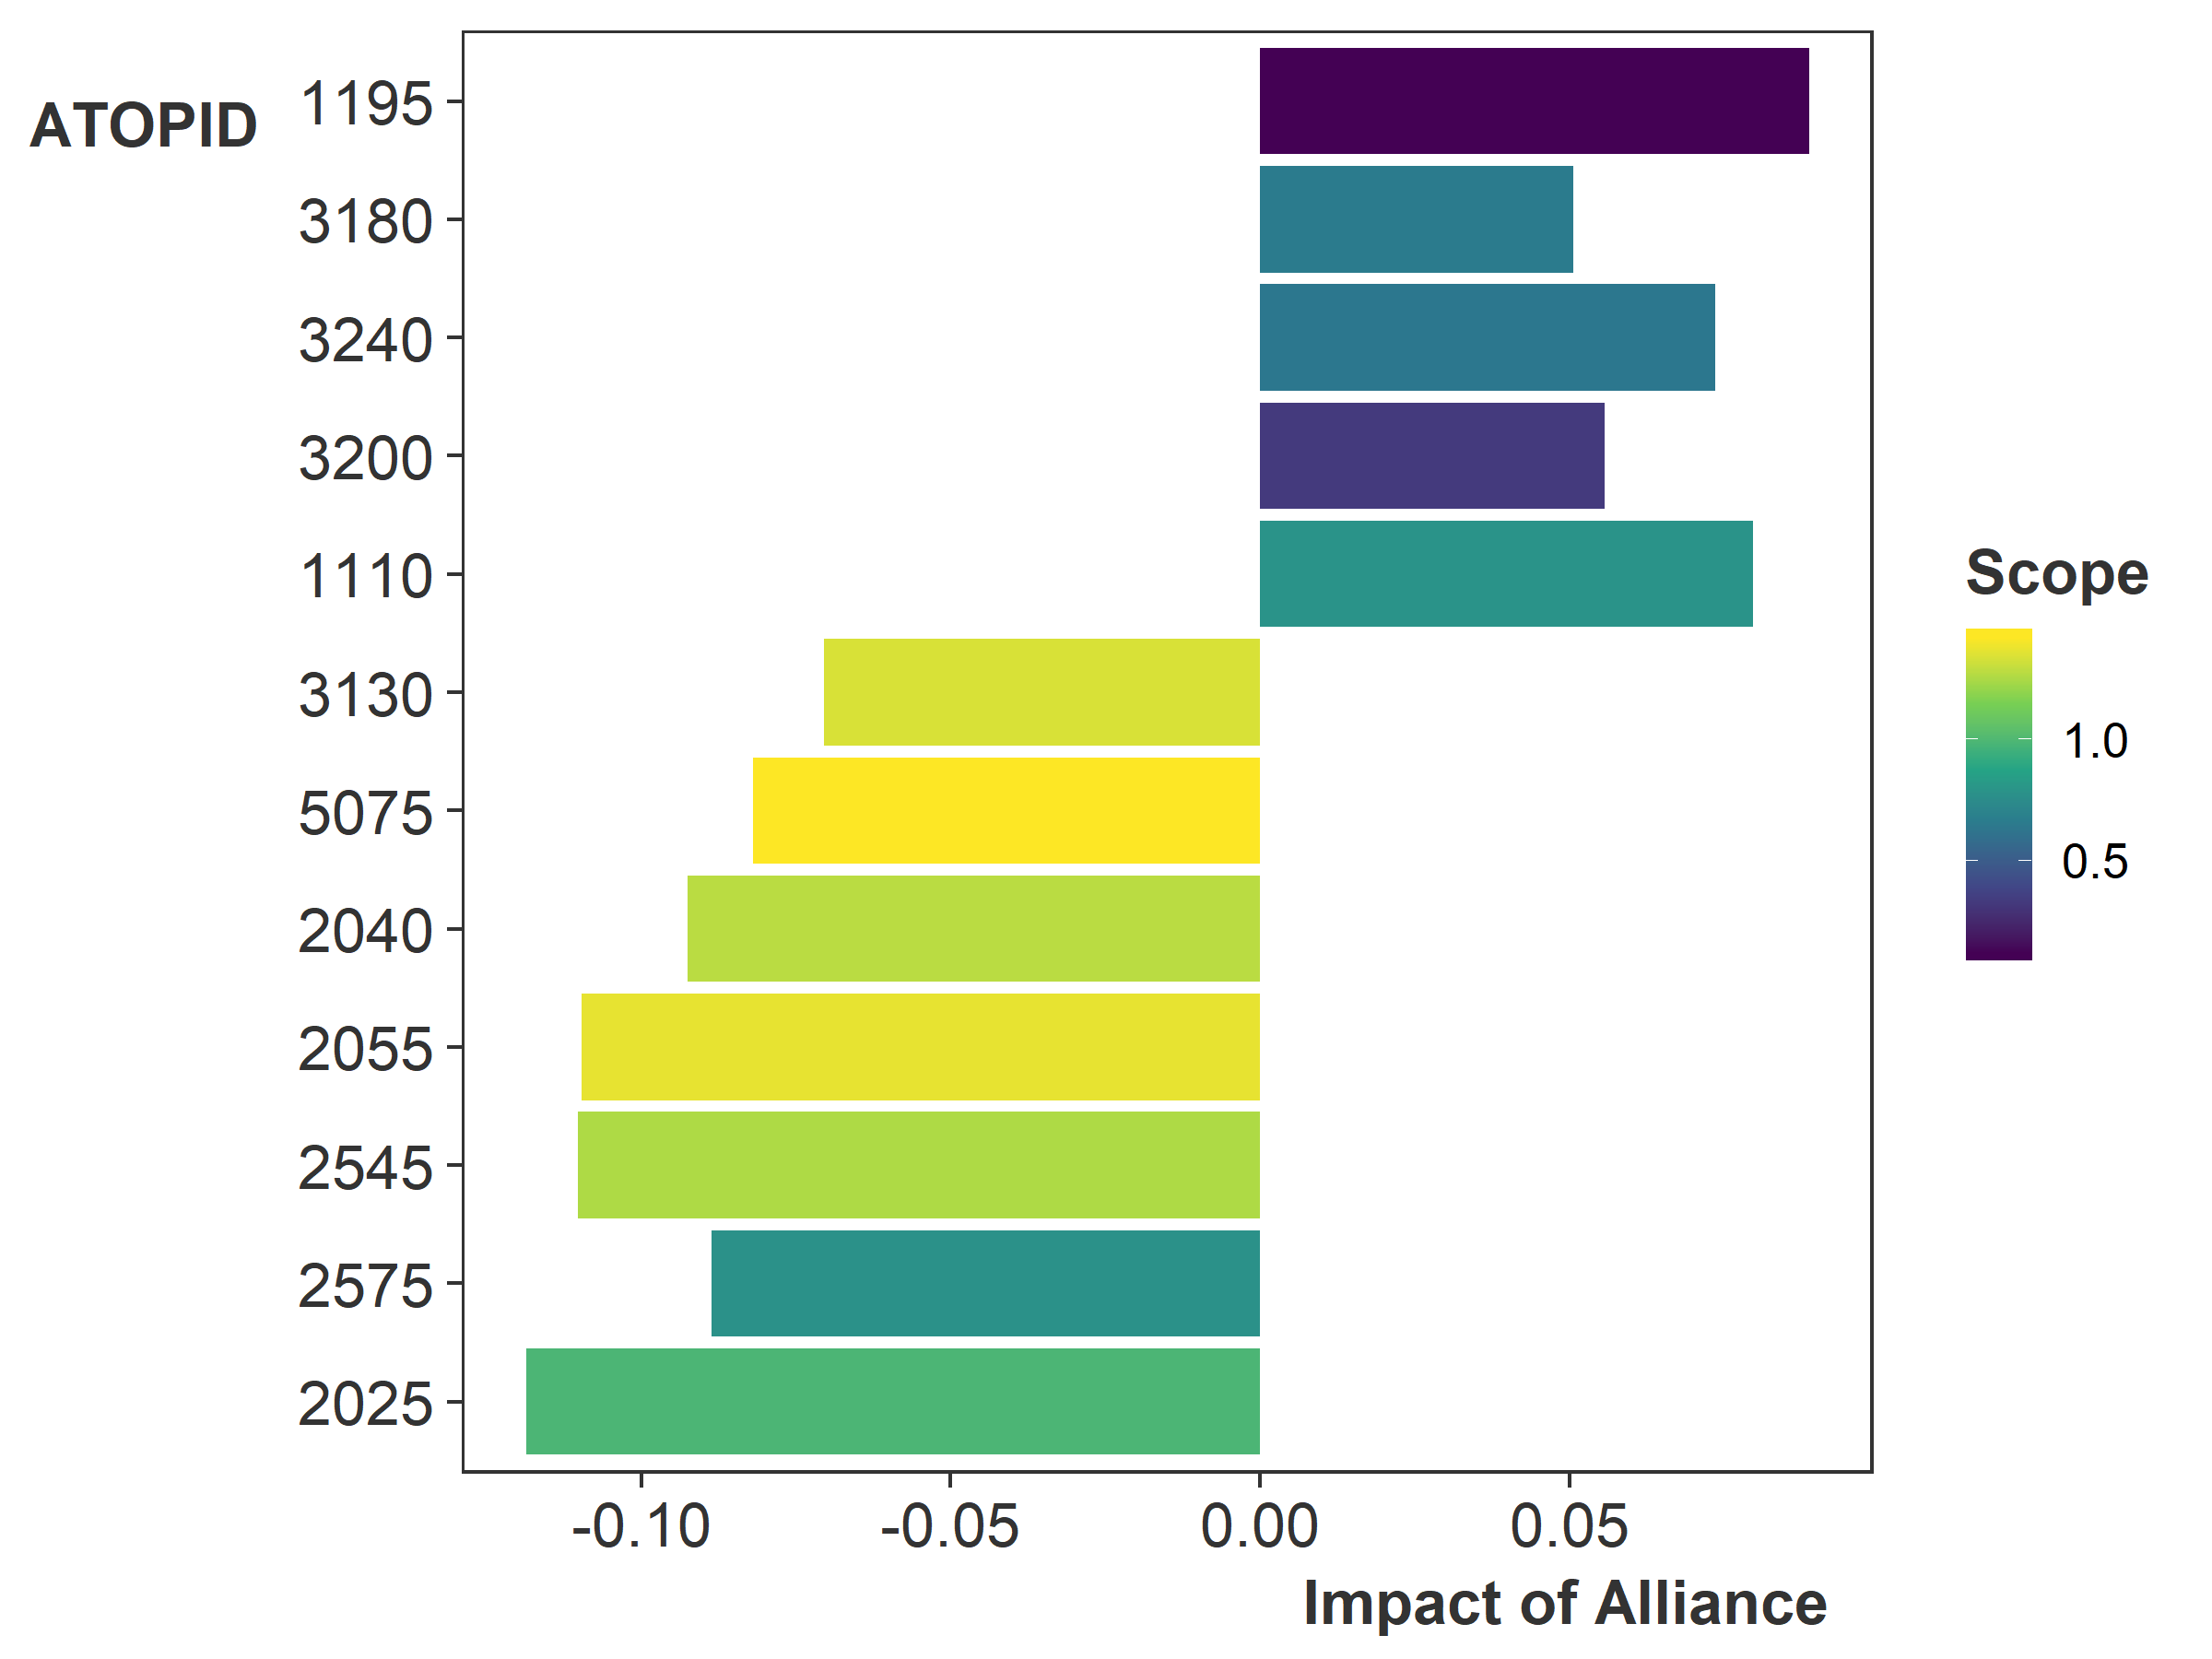
\includegraphics[width=0.95\textwidth]{non-zero-maj.png}
	\label{fig:non-zero-maj}
\end{figure}


\end{frame}

%------------------------------------------------

\begin{frame}{Notable Non-Major Power Alliances}


\begin{figure}
	\centering
		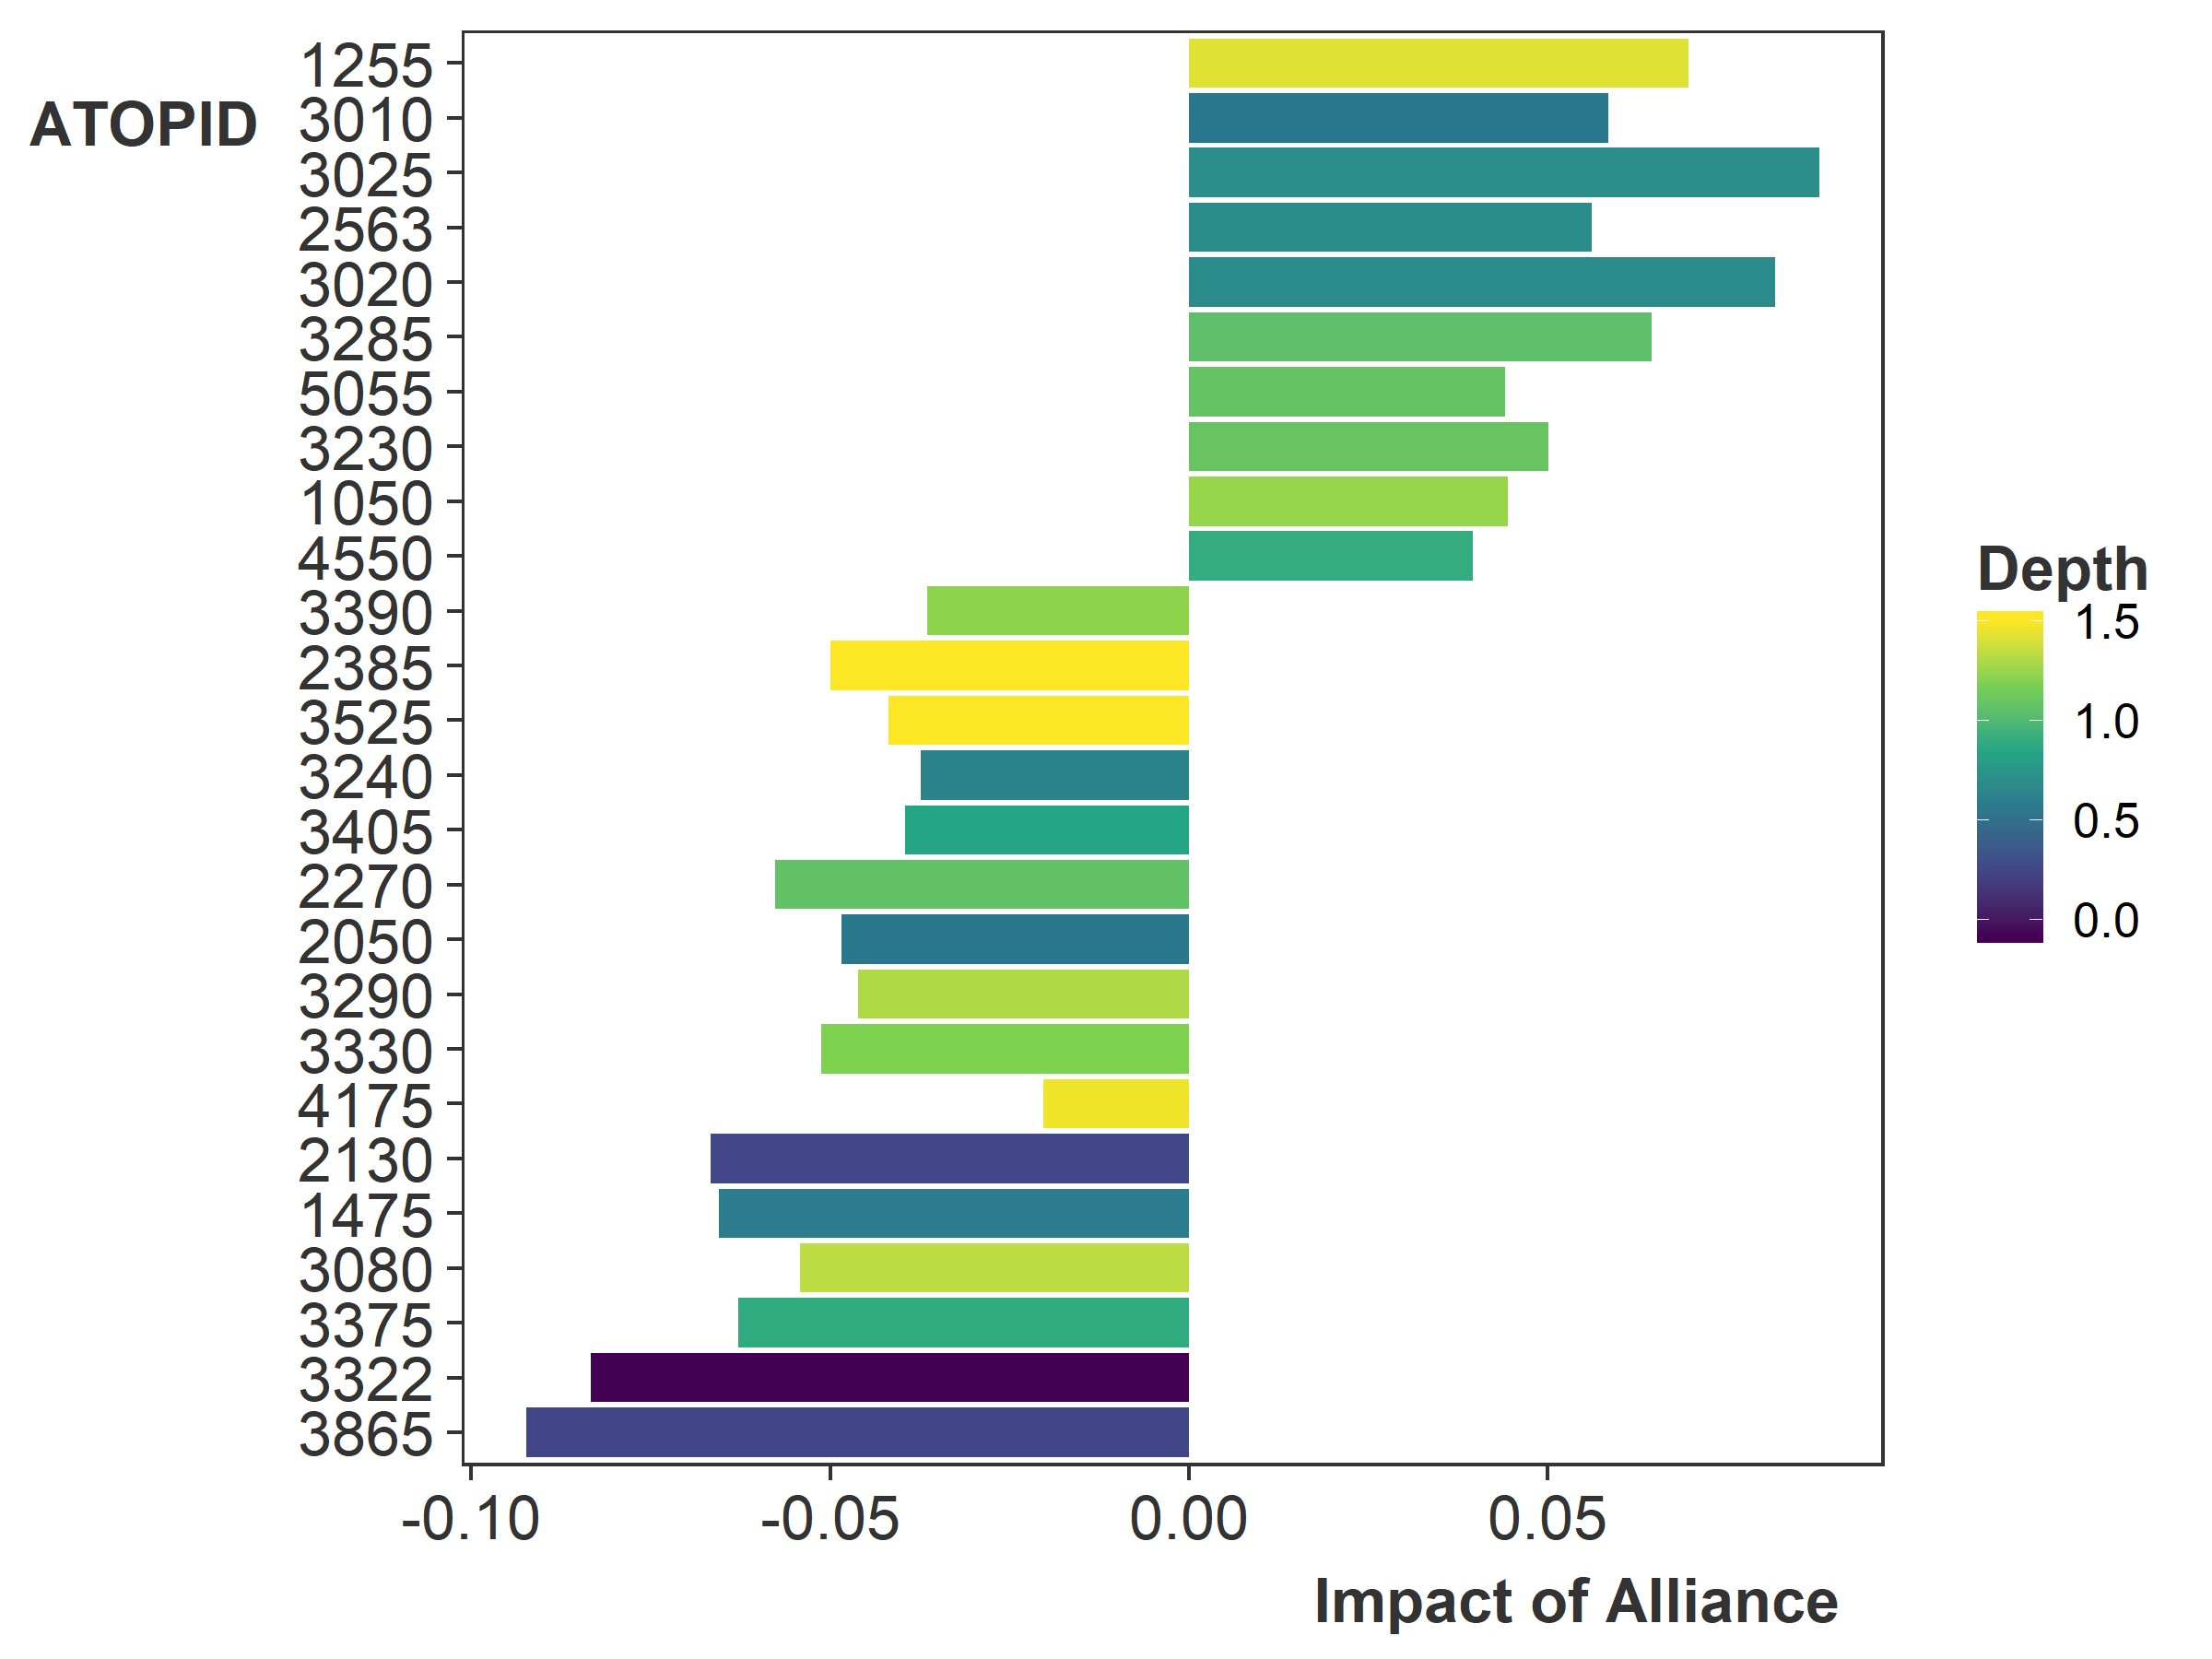
\includegraphics[width=0.95\textwidth]{non-zero-min.png}
	\label{fig:non-zero-min}
\end{figure}


\end{frame}


%------------------------------------------------

\begin{frame}{Impact of US Alliance on Non-major Power Military Spending} 

\begin{figure}
	\centering
		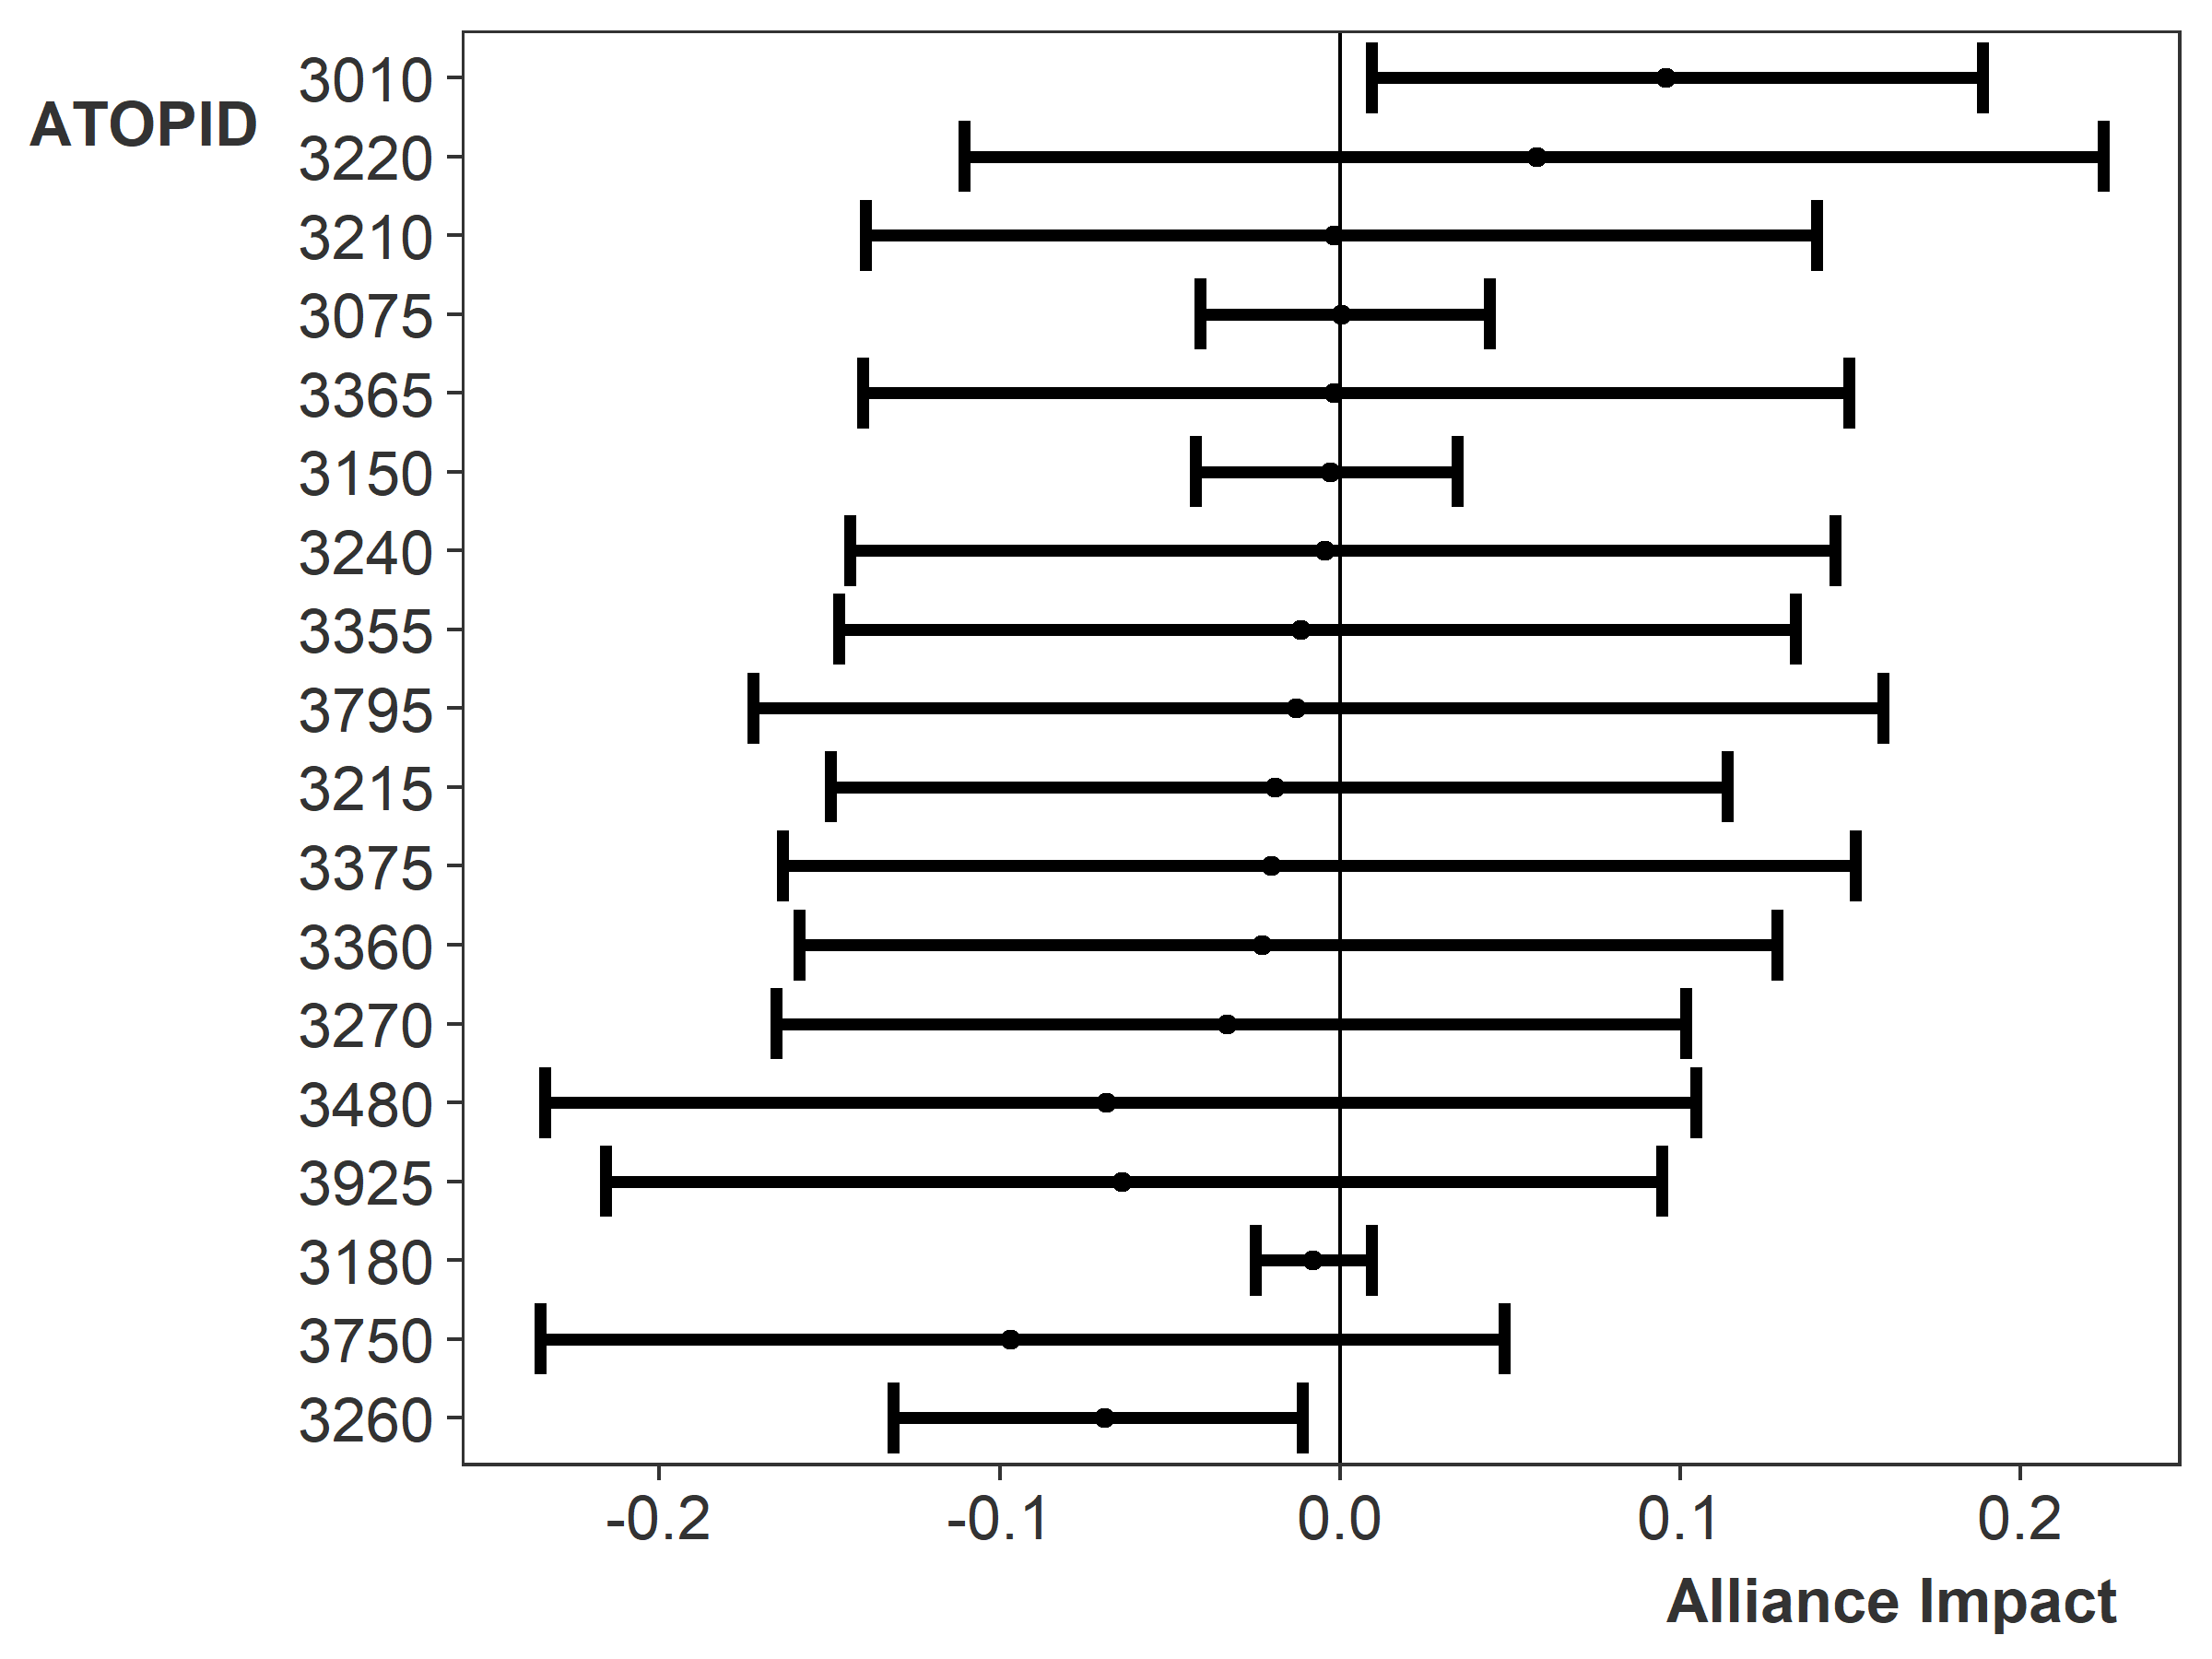
\includegraphics[width=0.85\textwidth]{lambda-us-min.png}
\end{figure}


\end{frame}

%------------------------------------------------

\begin{frame}{NATO} 

\begin{figure}
	\centering
		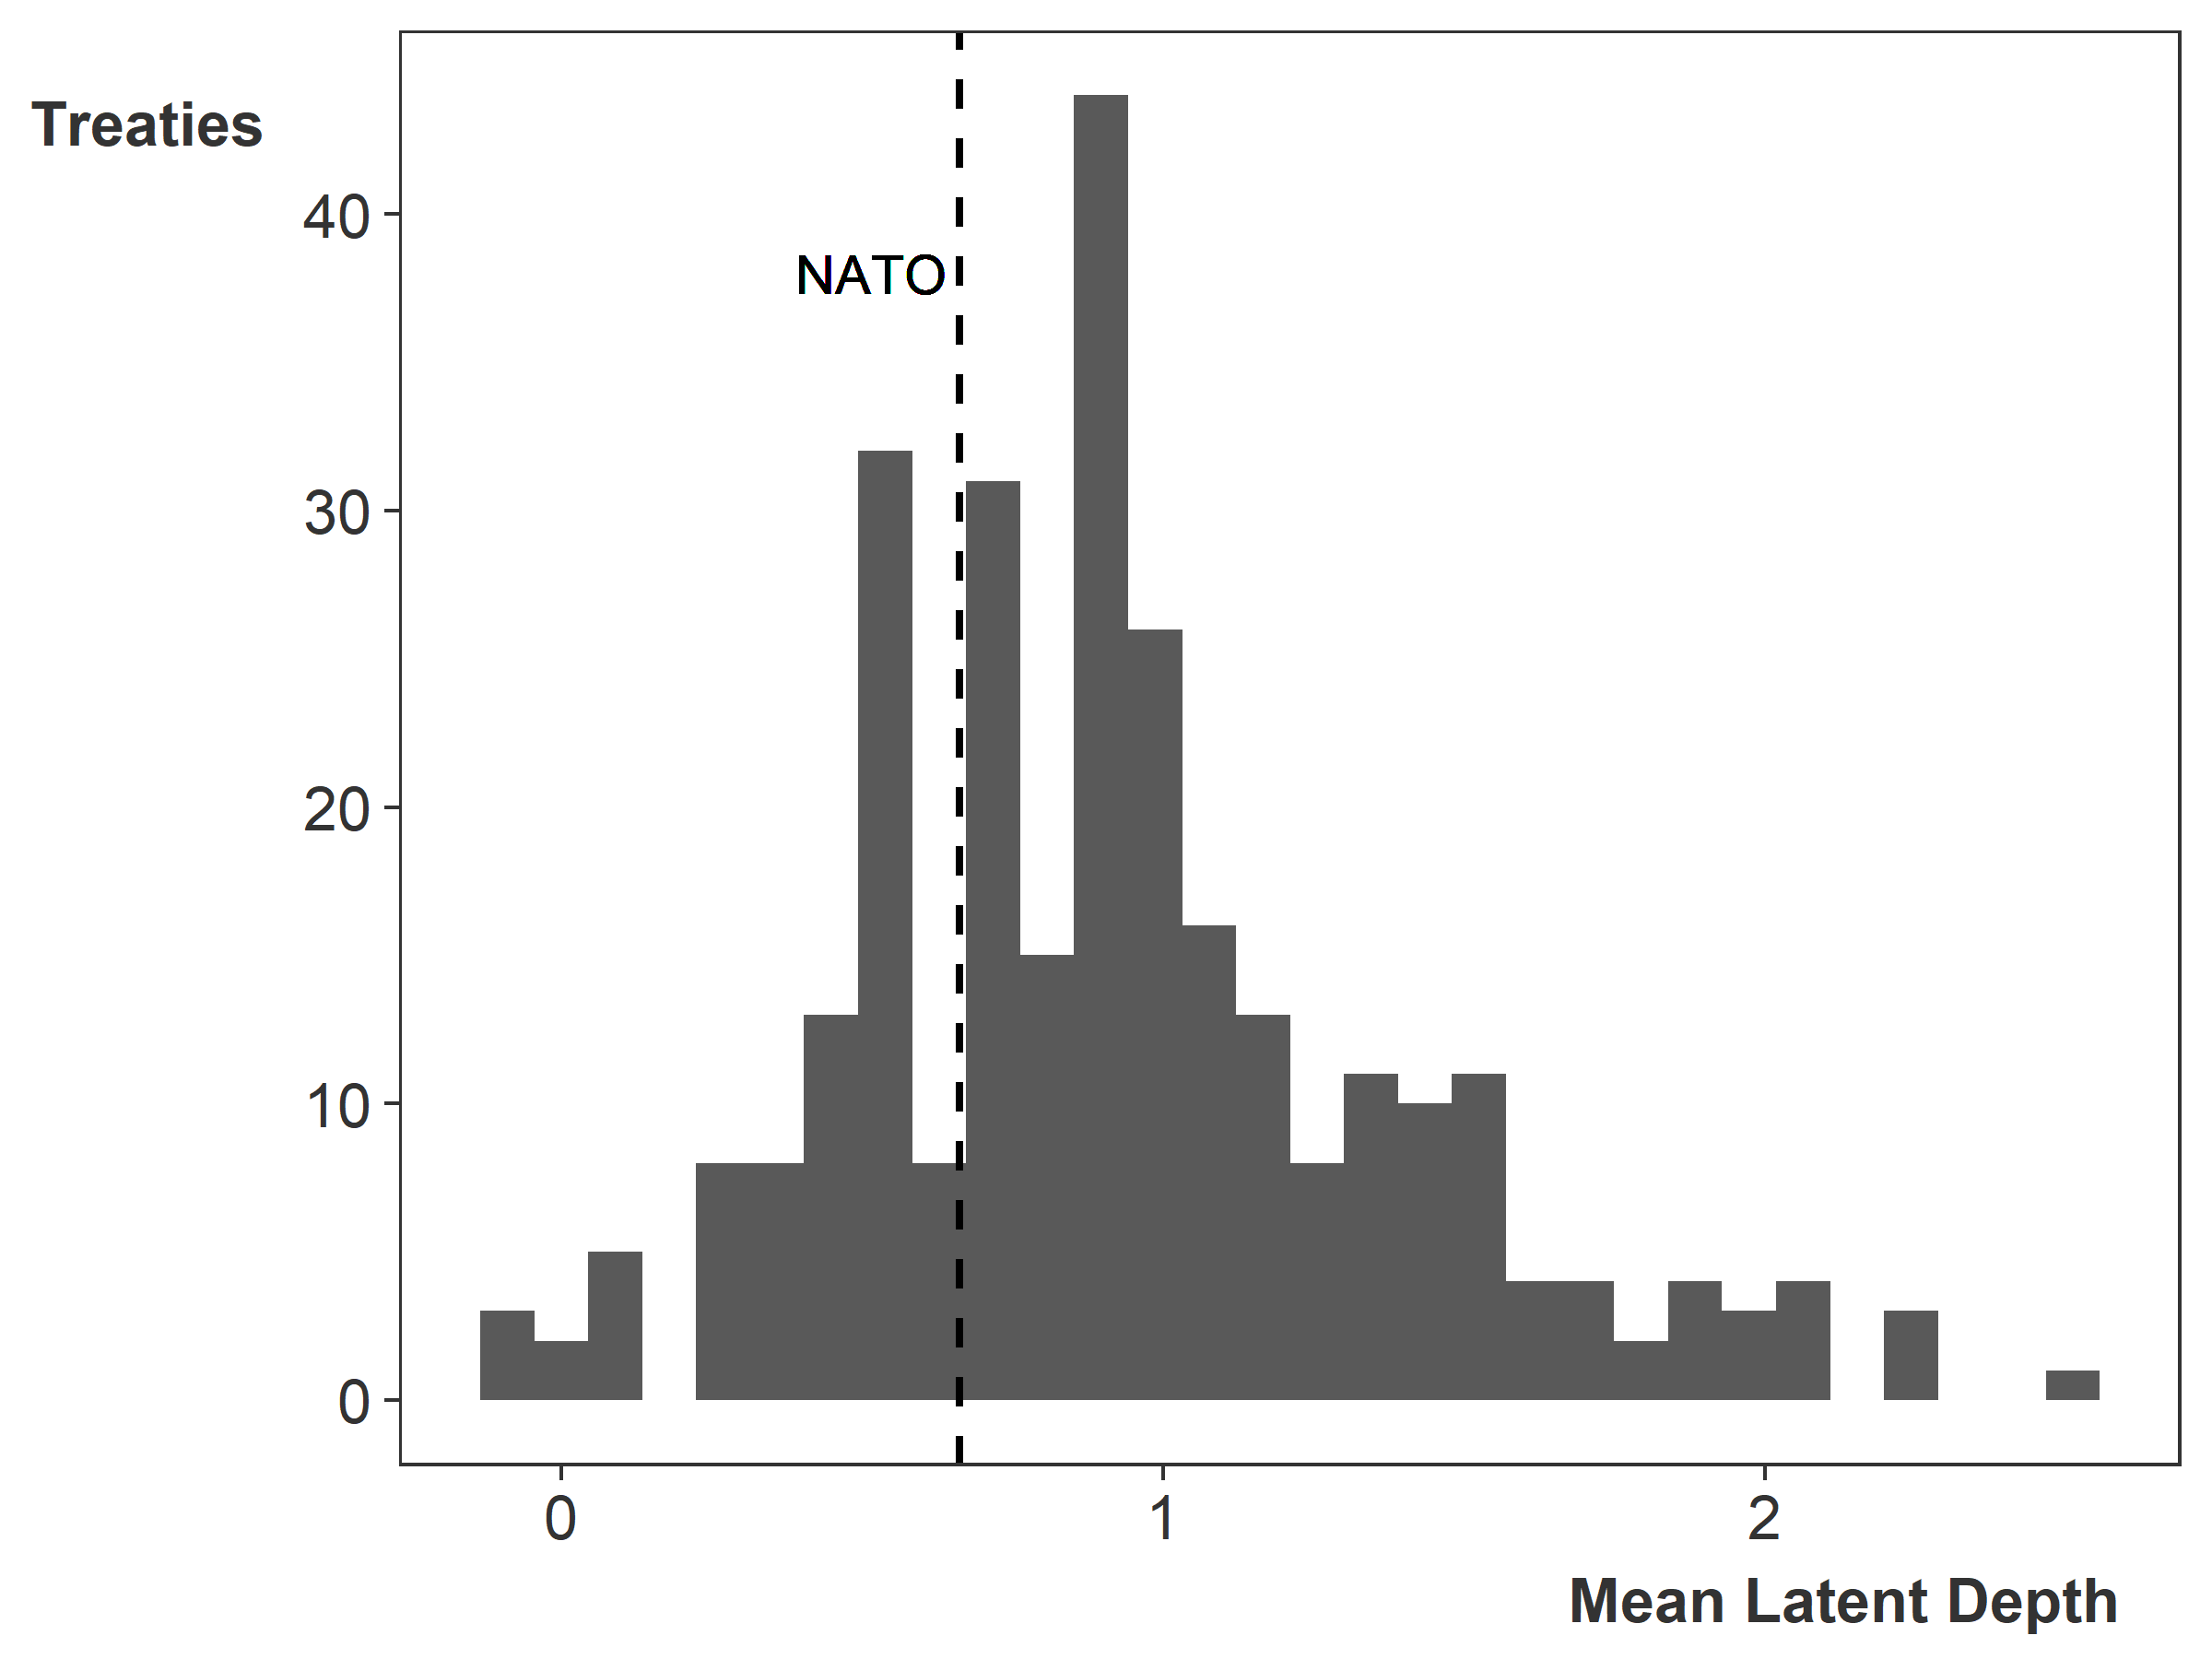
\includegraphics[width=0.95\textwidth]{ld-hist-nato.png}
\end{figure}


 \end{frame}


%------------------------------------------------

\begin{frame}{Non-Major Powers in NATO: Belgium}


\begin{figure}
	\centering
		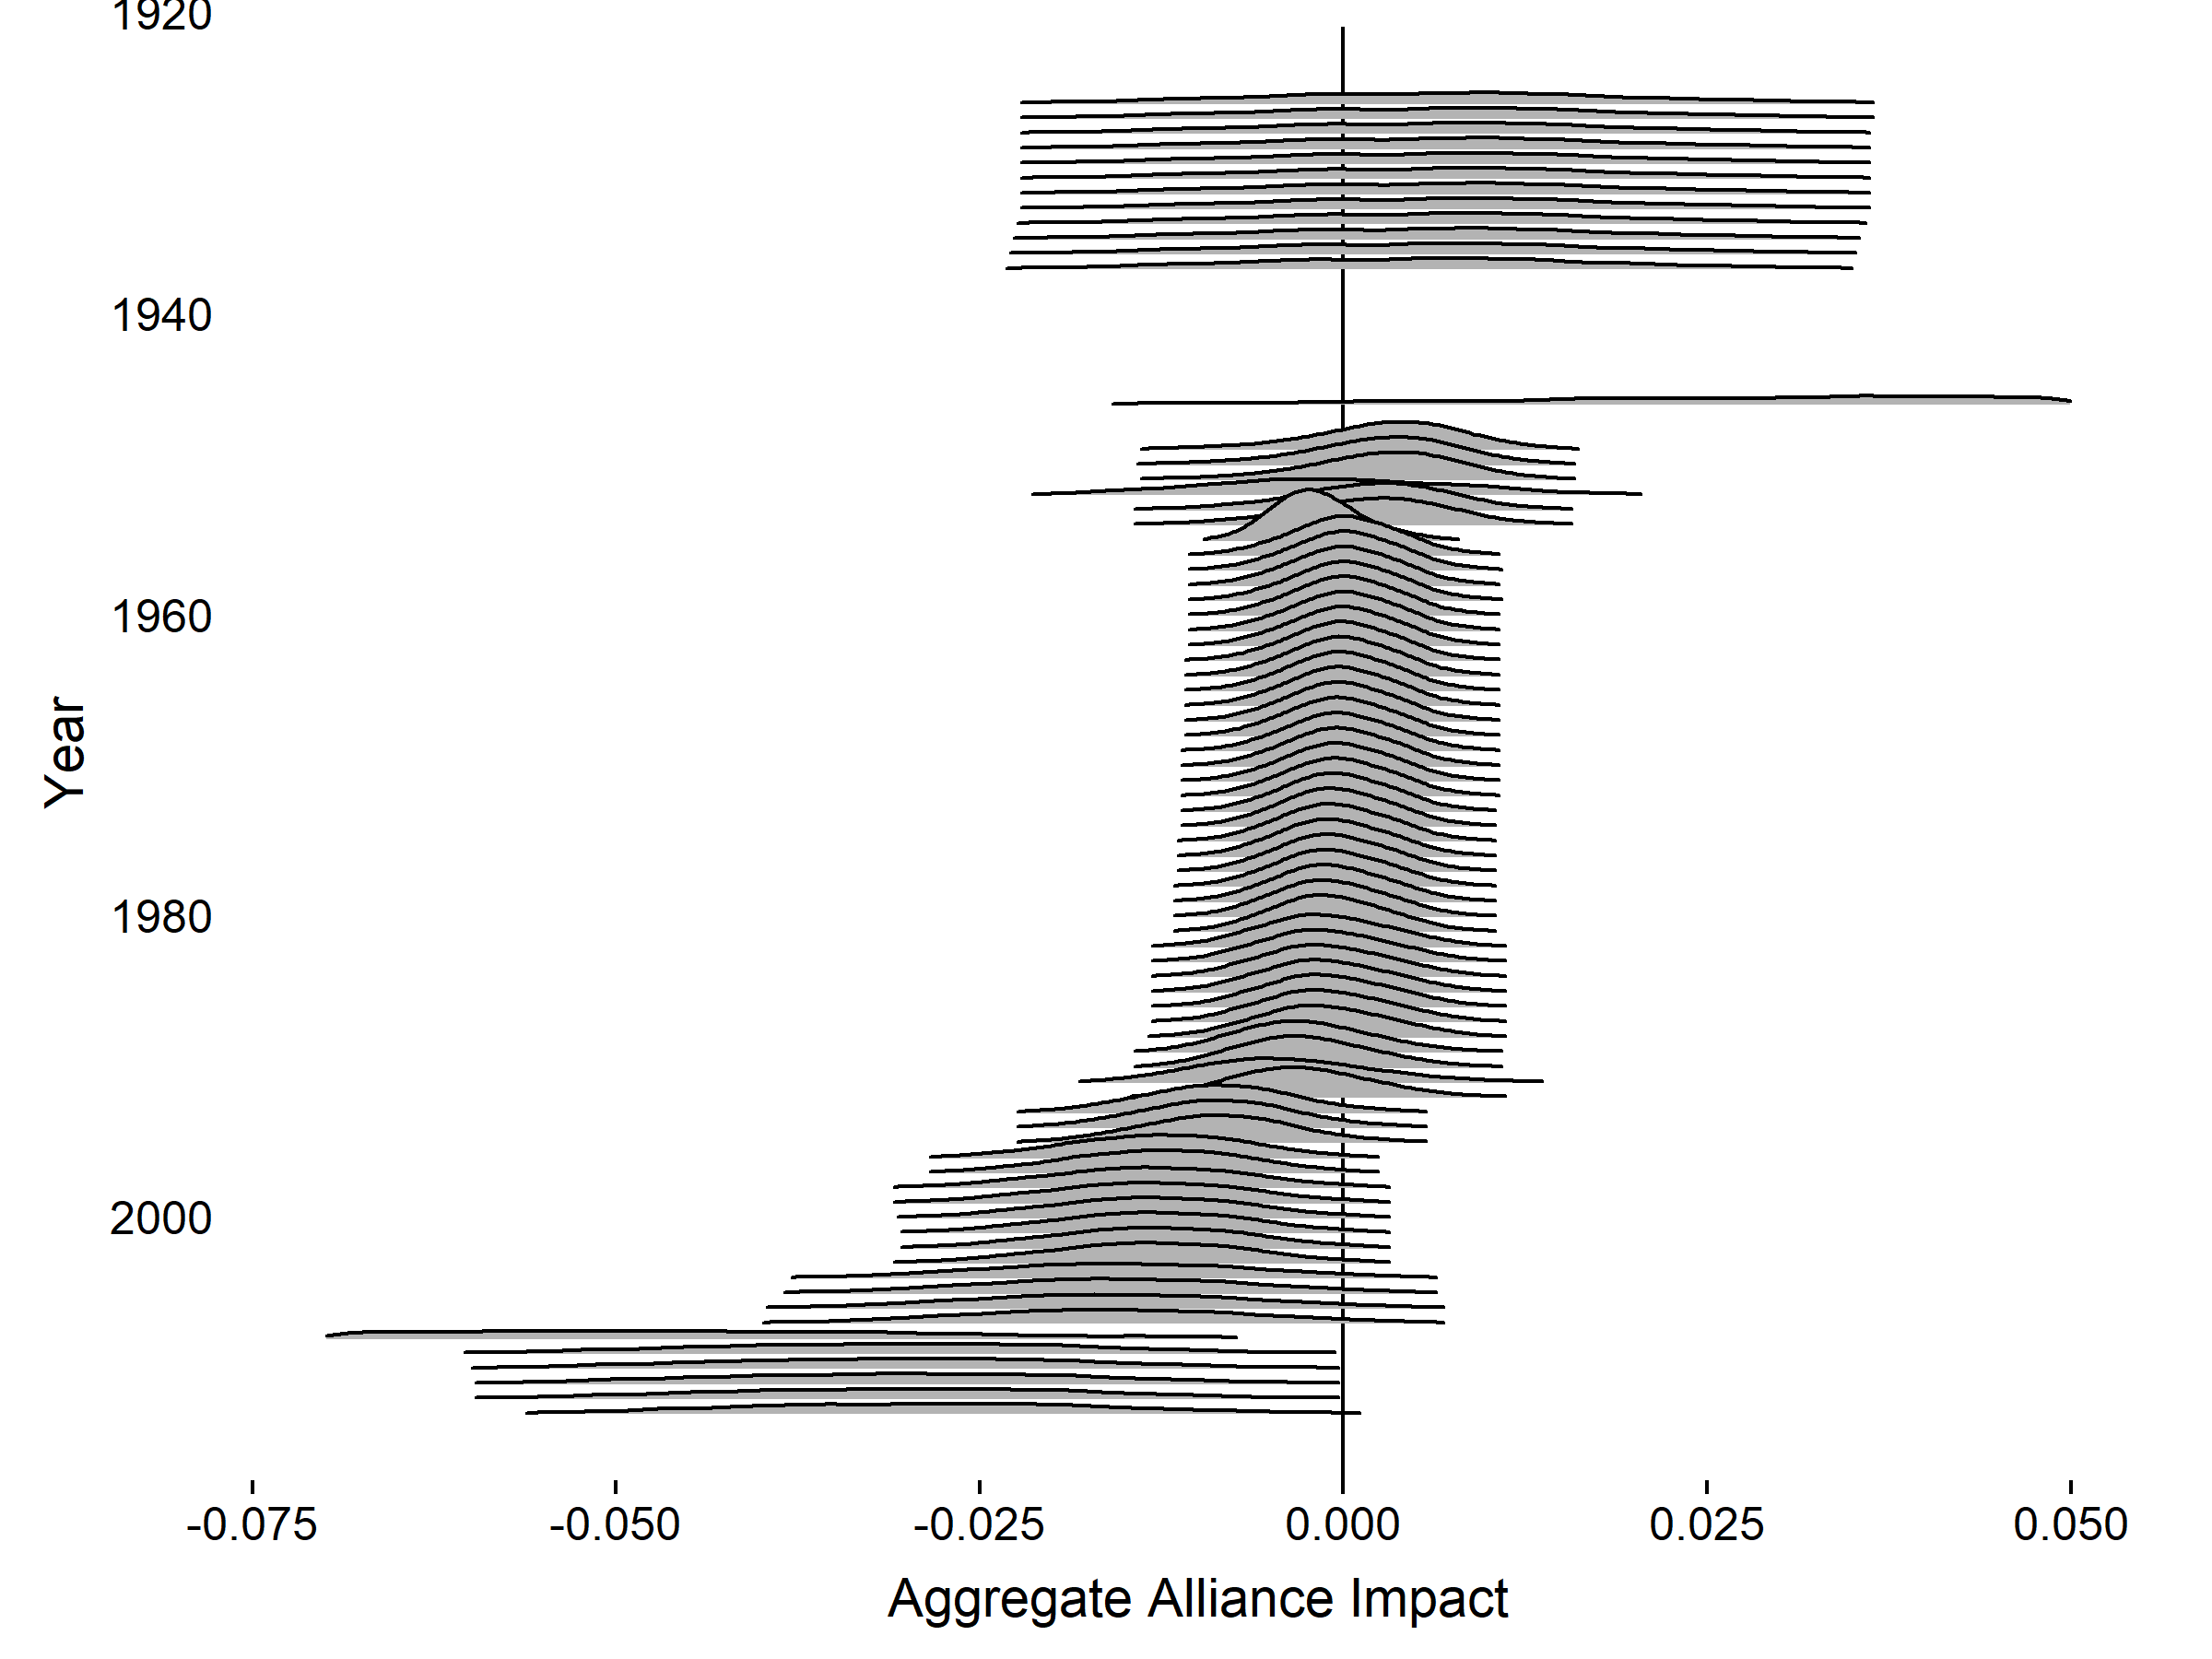
\includegraphics[width=0.95\textwidth]{bel-agg-imp.png}
\end{figure}


\end{frame}


%------------------------------------------------

\begin{frame}{Impact of NATO on Belgium}


\begin{figure}
	\centering
		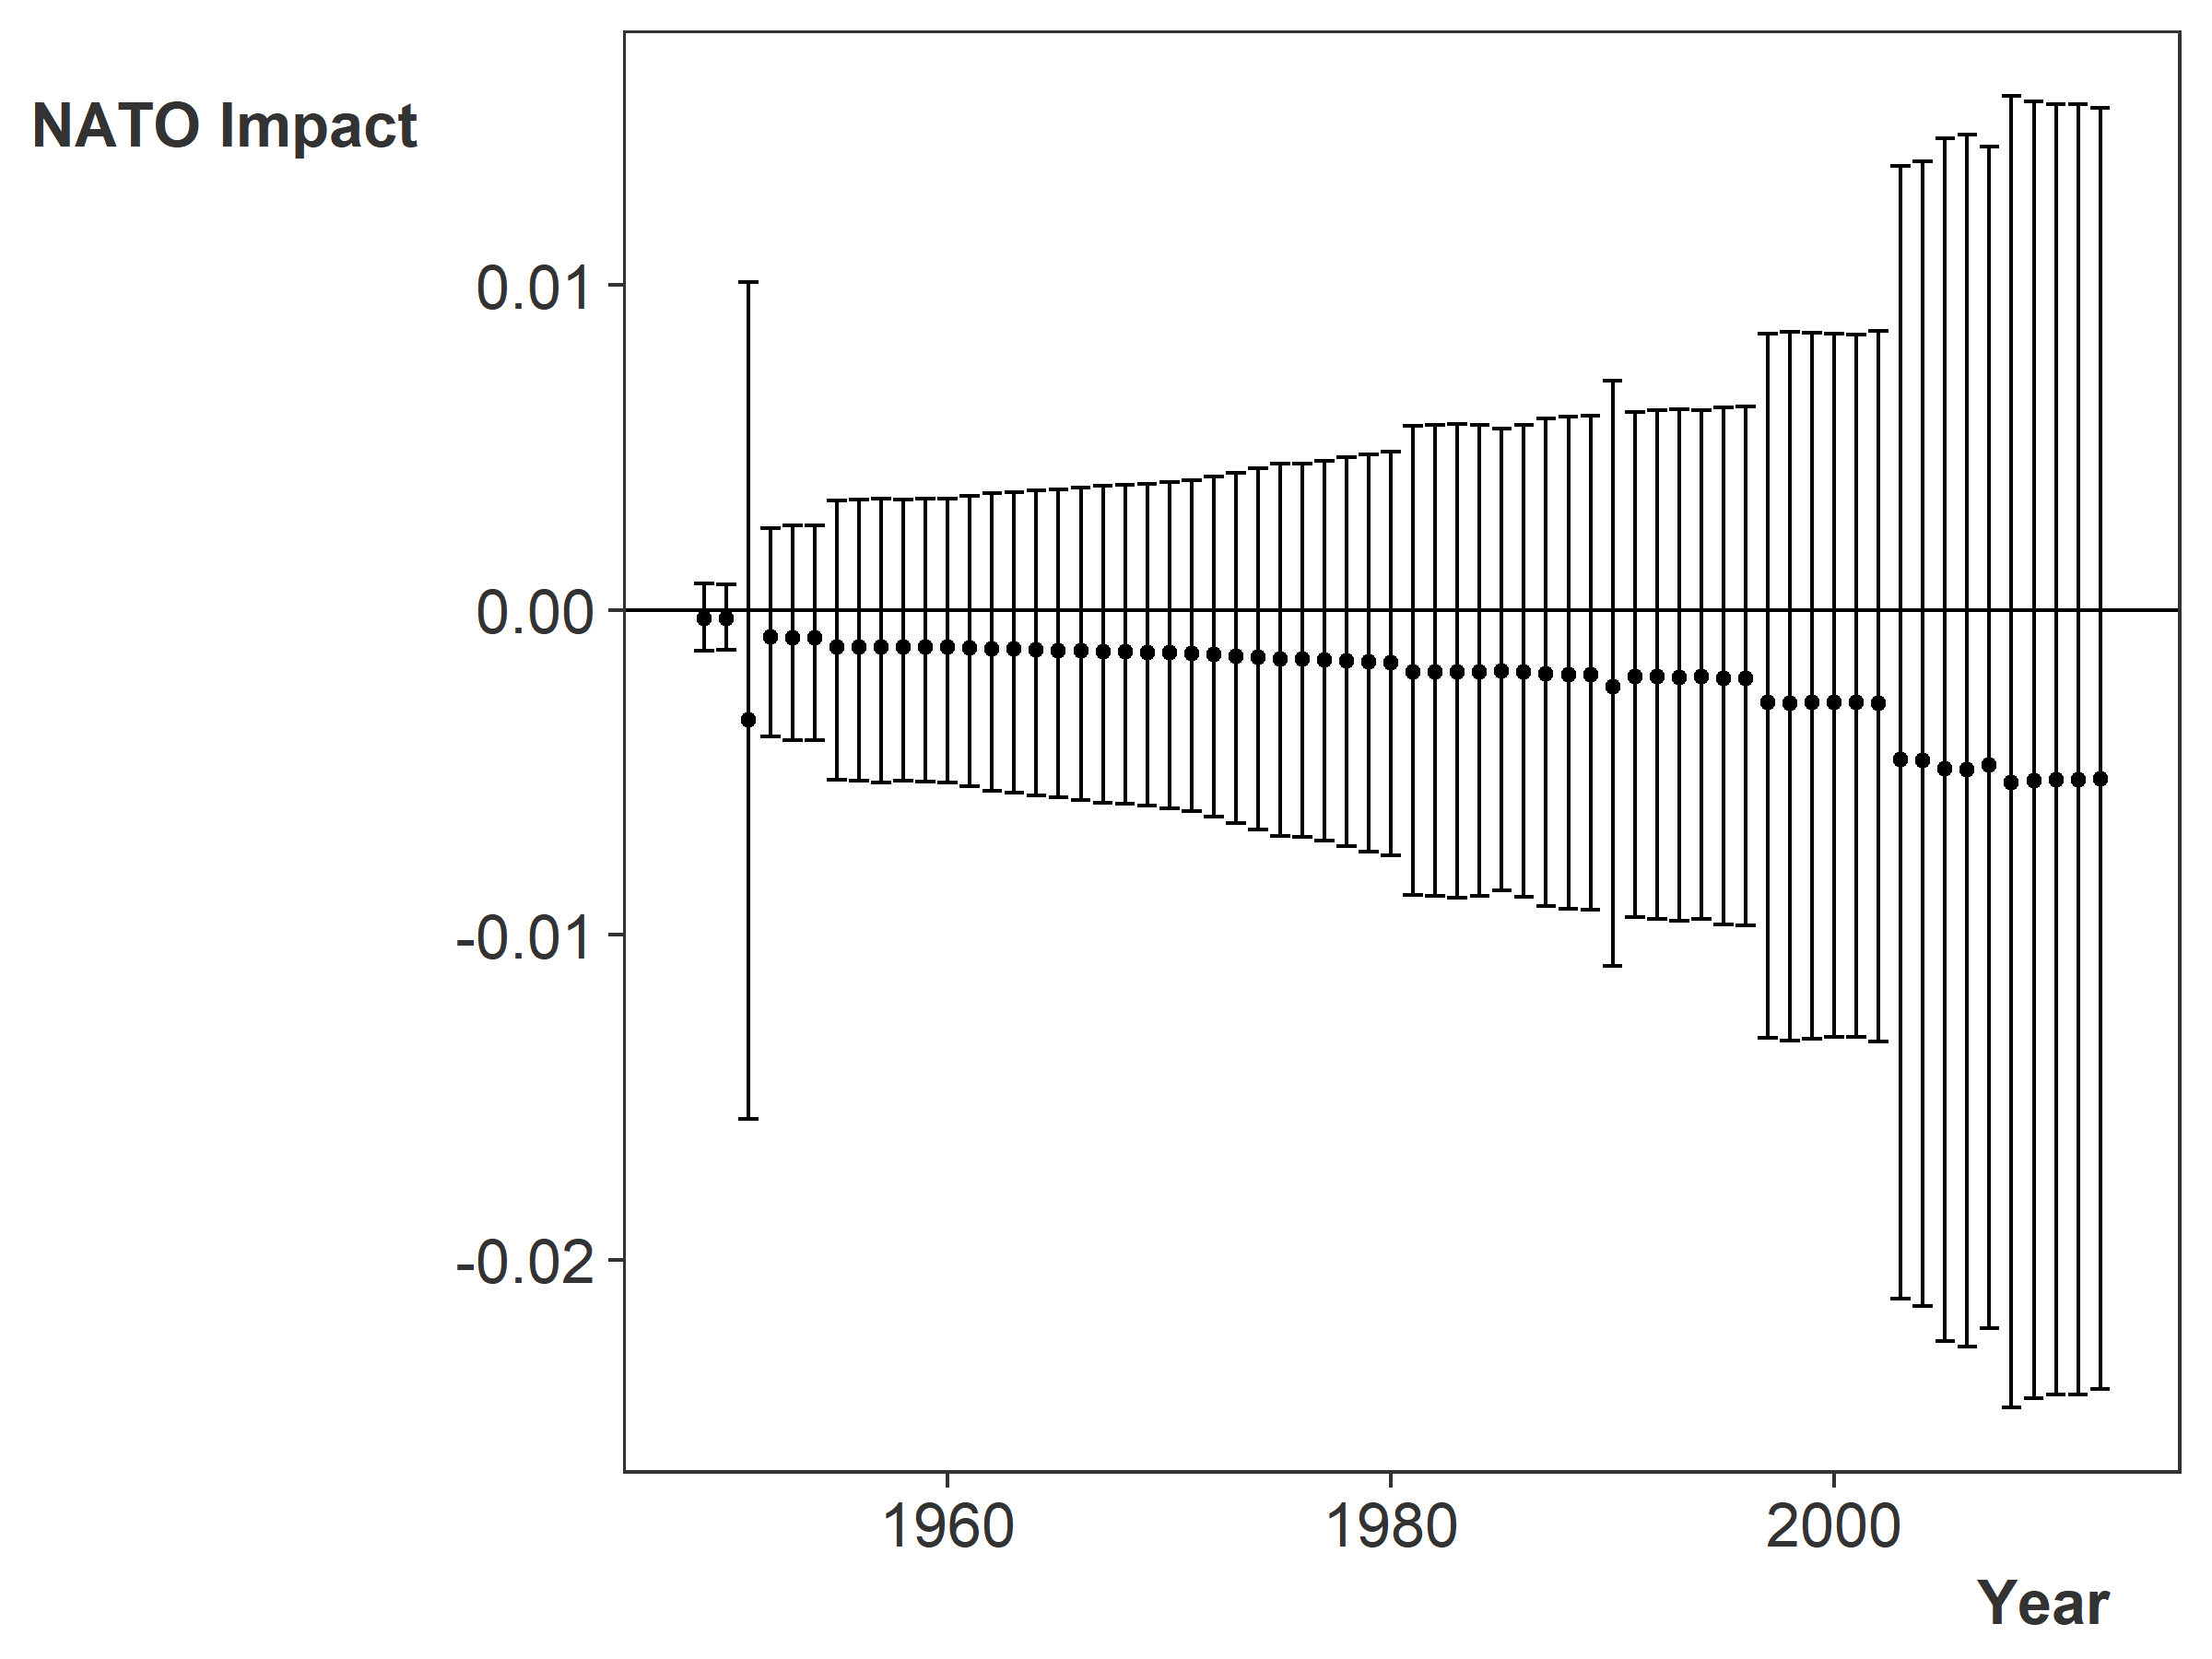
\includegraphics[width=0.95\textwidth]{bel-nato-imp.png}
\end{figure}


\end{frame}


%------------------------------------------------

\begin{frame}{Impact of EU on Belgium}


\begin{figure}
	\centering
		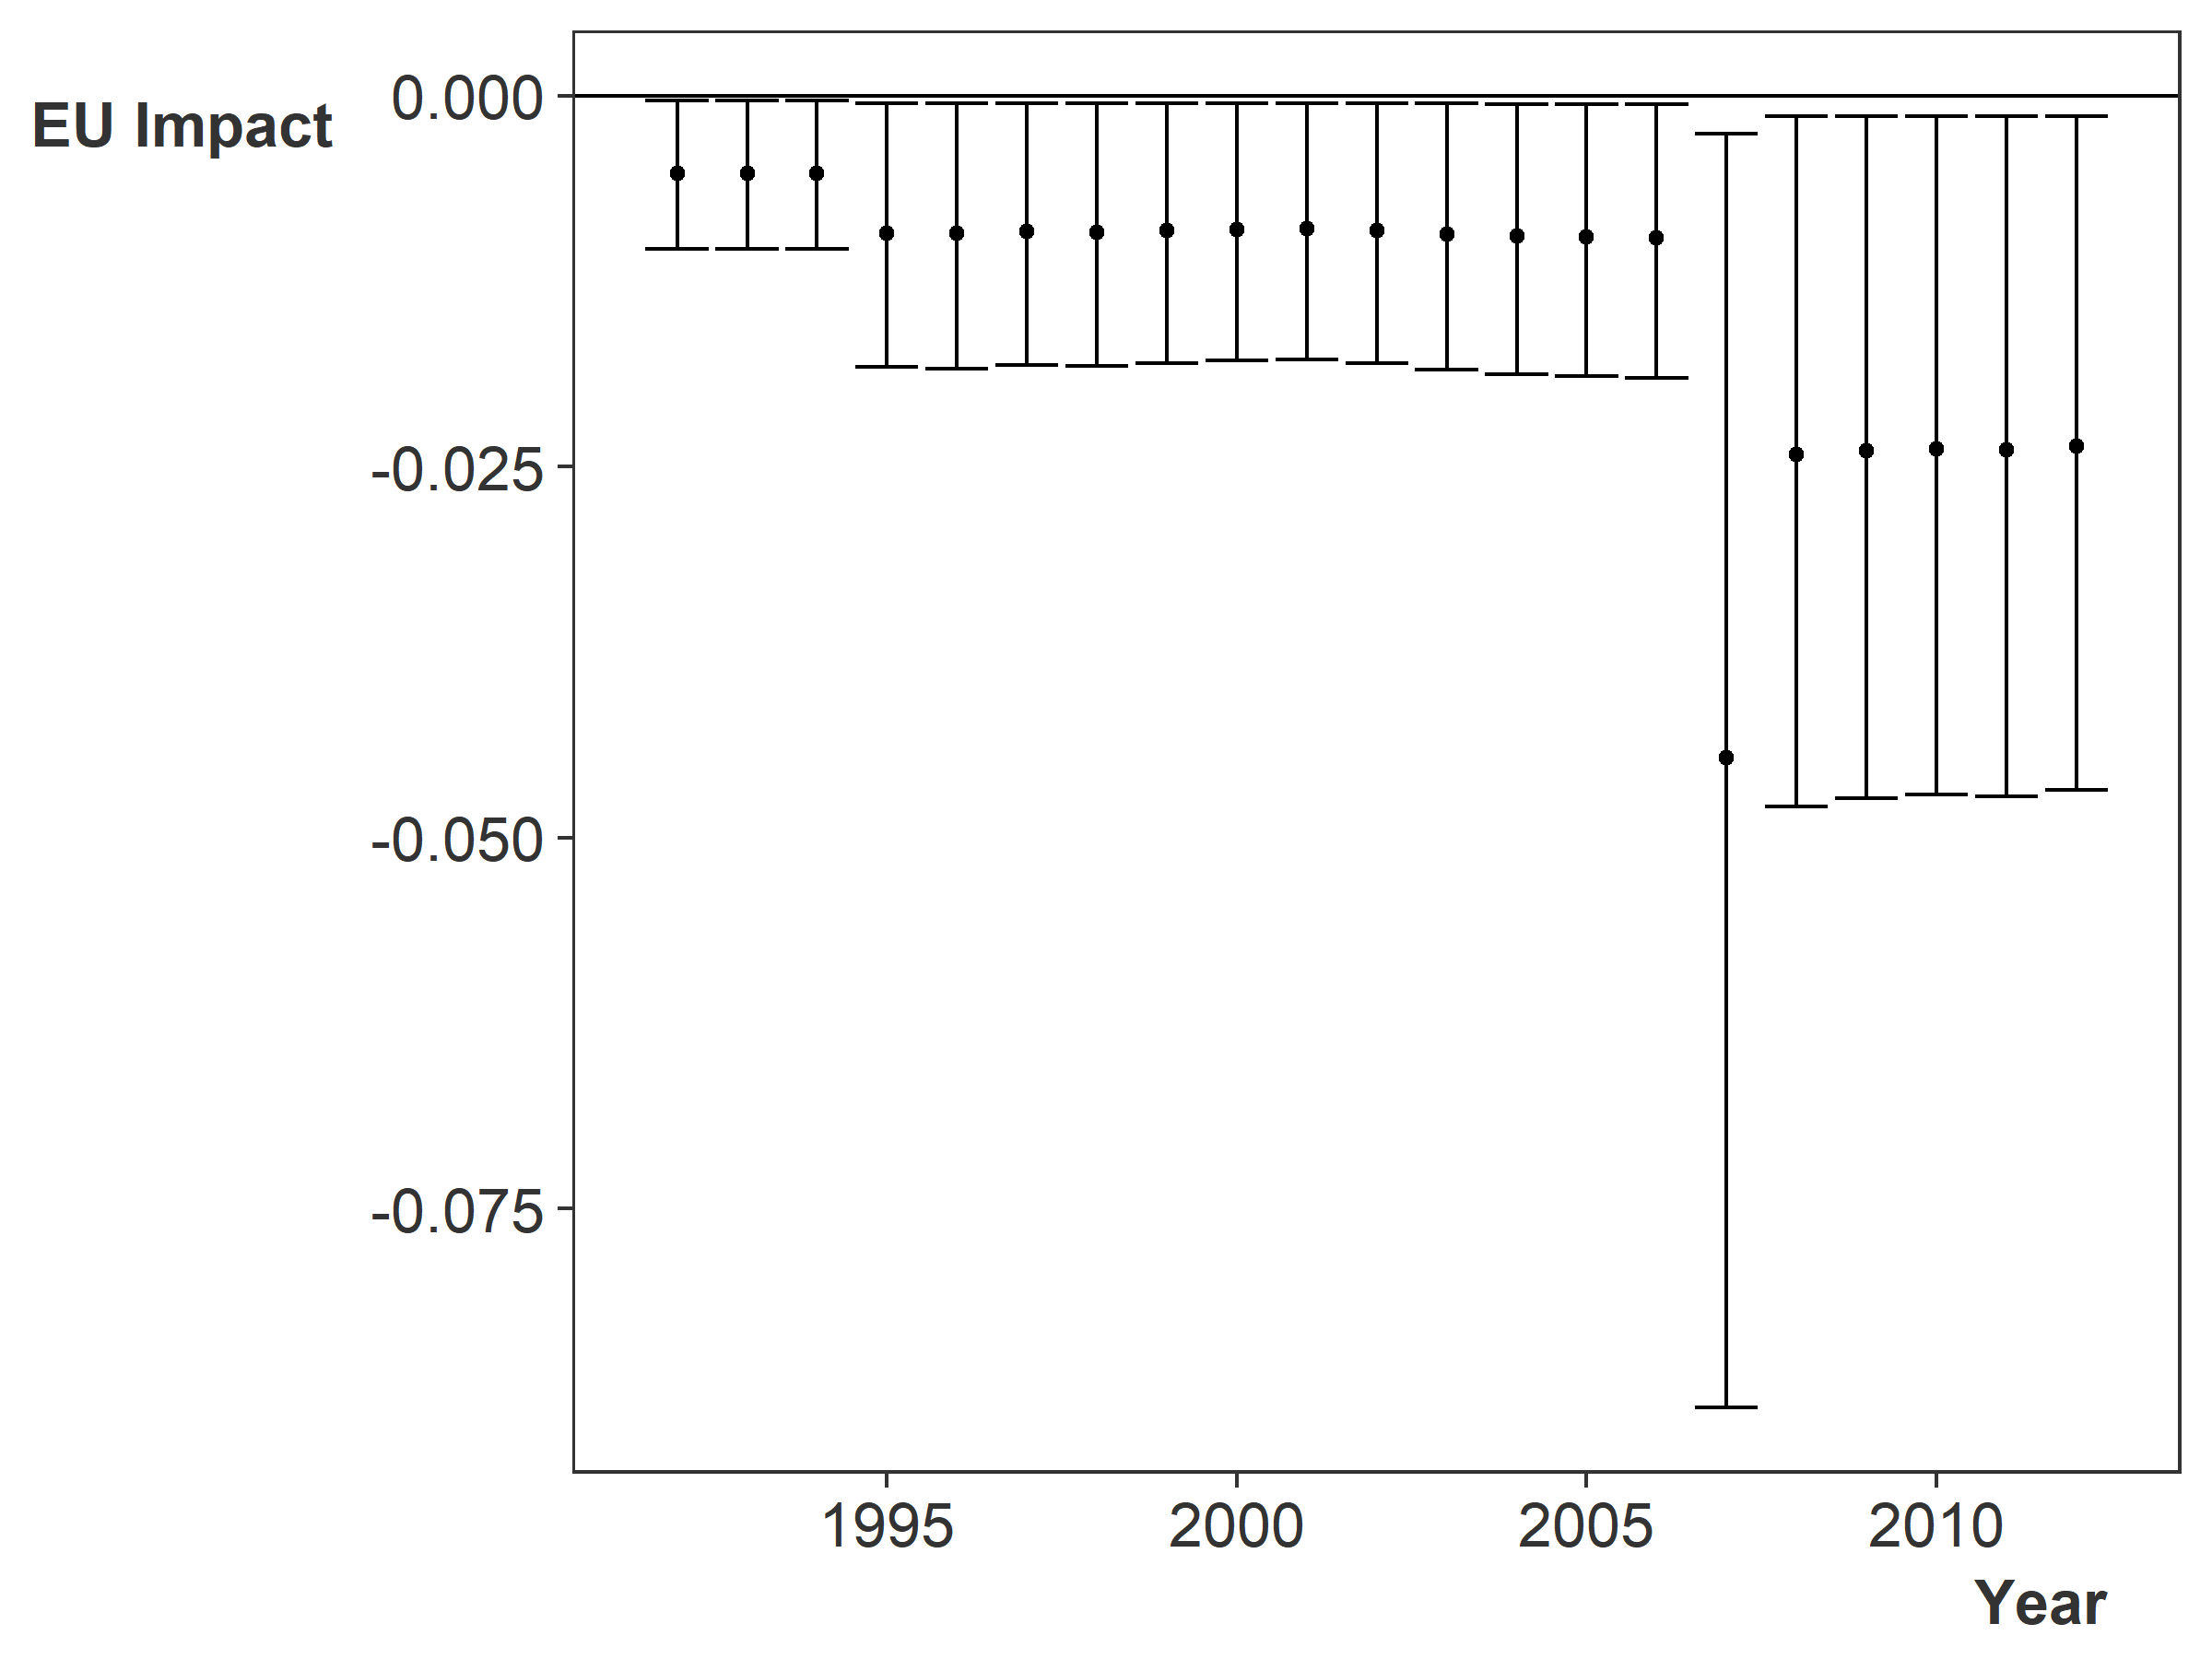
\includegraphics[width=0.95\textwidth]{bel-eu-imp.png}
\end{figure}


\end{frame}




%------------------------------------------------

\begin{frame}{Varying Slopes Model}

Within each of the $j$ groups of state capability, for $i$ in $1 ... n_j$: 
\begin{equation*}
y_i \sim student_t(\nu_j, \alpha_j + \alpha^{st} + \alpha^{yr} +\textbf{W}_{i} \gamma  + \textbf{Z}_{ji} \lambda_{j}, \sigma_j) 
\end{equation*} 

\begin{equation*}
\lambda_{j} \sim N(\theta_{j}, \sigma^{all}_{j})
\end{equation*} 

\begin{equation*}
\theta_{j} = \alpha^{all}_{j} + \textbf{X} \beta_j
\end{equation*}

I give $\beta_j$ a multivariate normal prior with prior scale $\tau$:
\begin{equation*}
\beta_j \sim MVN(\mu_{\beta_j}, \Sigma_{\beta}) 
\end{equation*}

\end{frame}


%------------------------------------------------

\begin{frame}{Varying Slopes Results: Depth}

\begin{figure}[htbp]
	\centering
		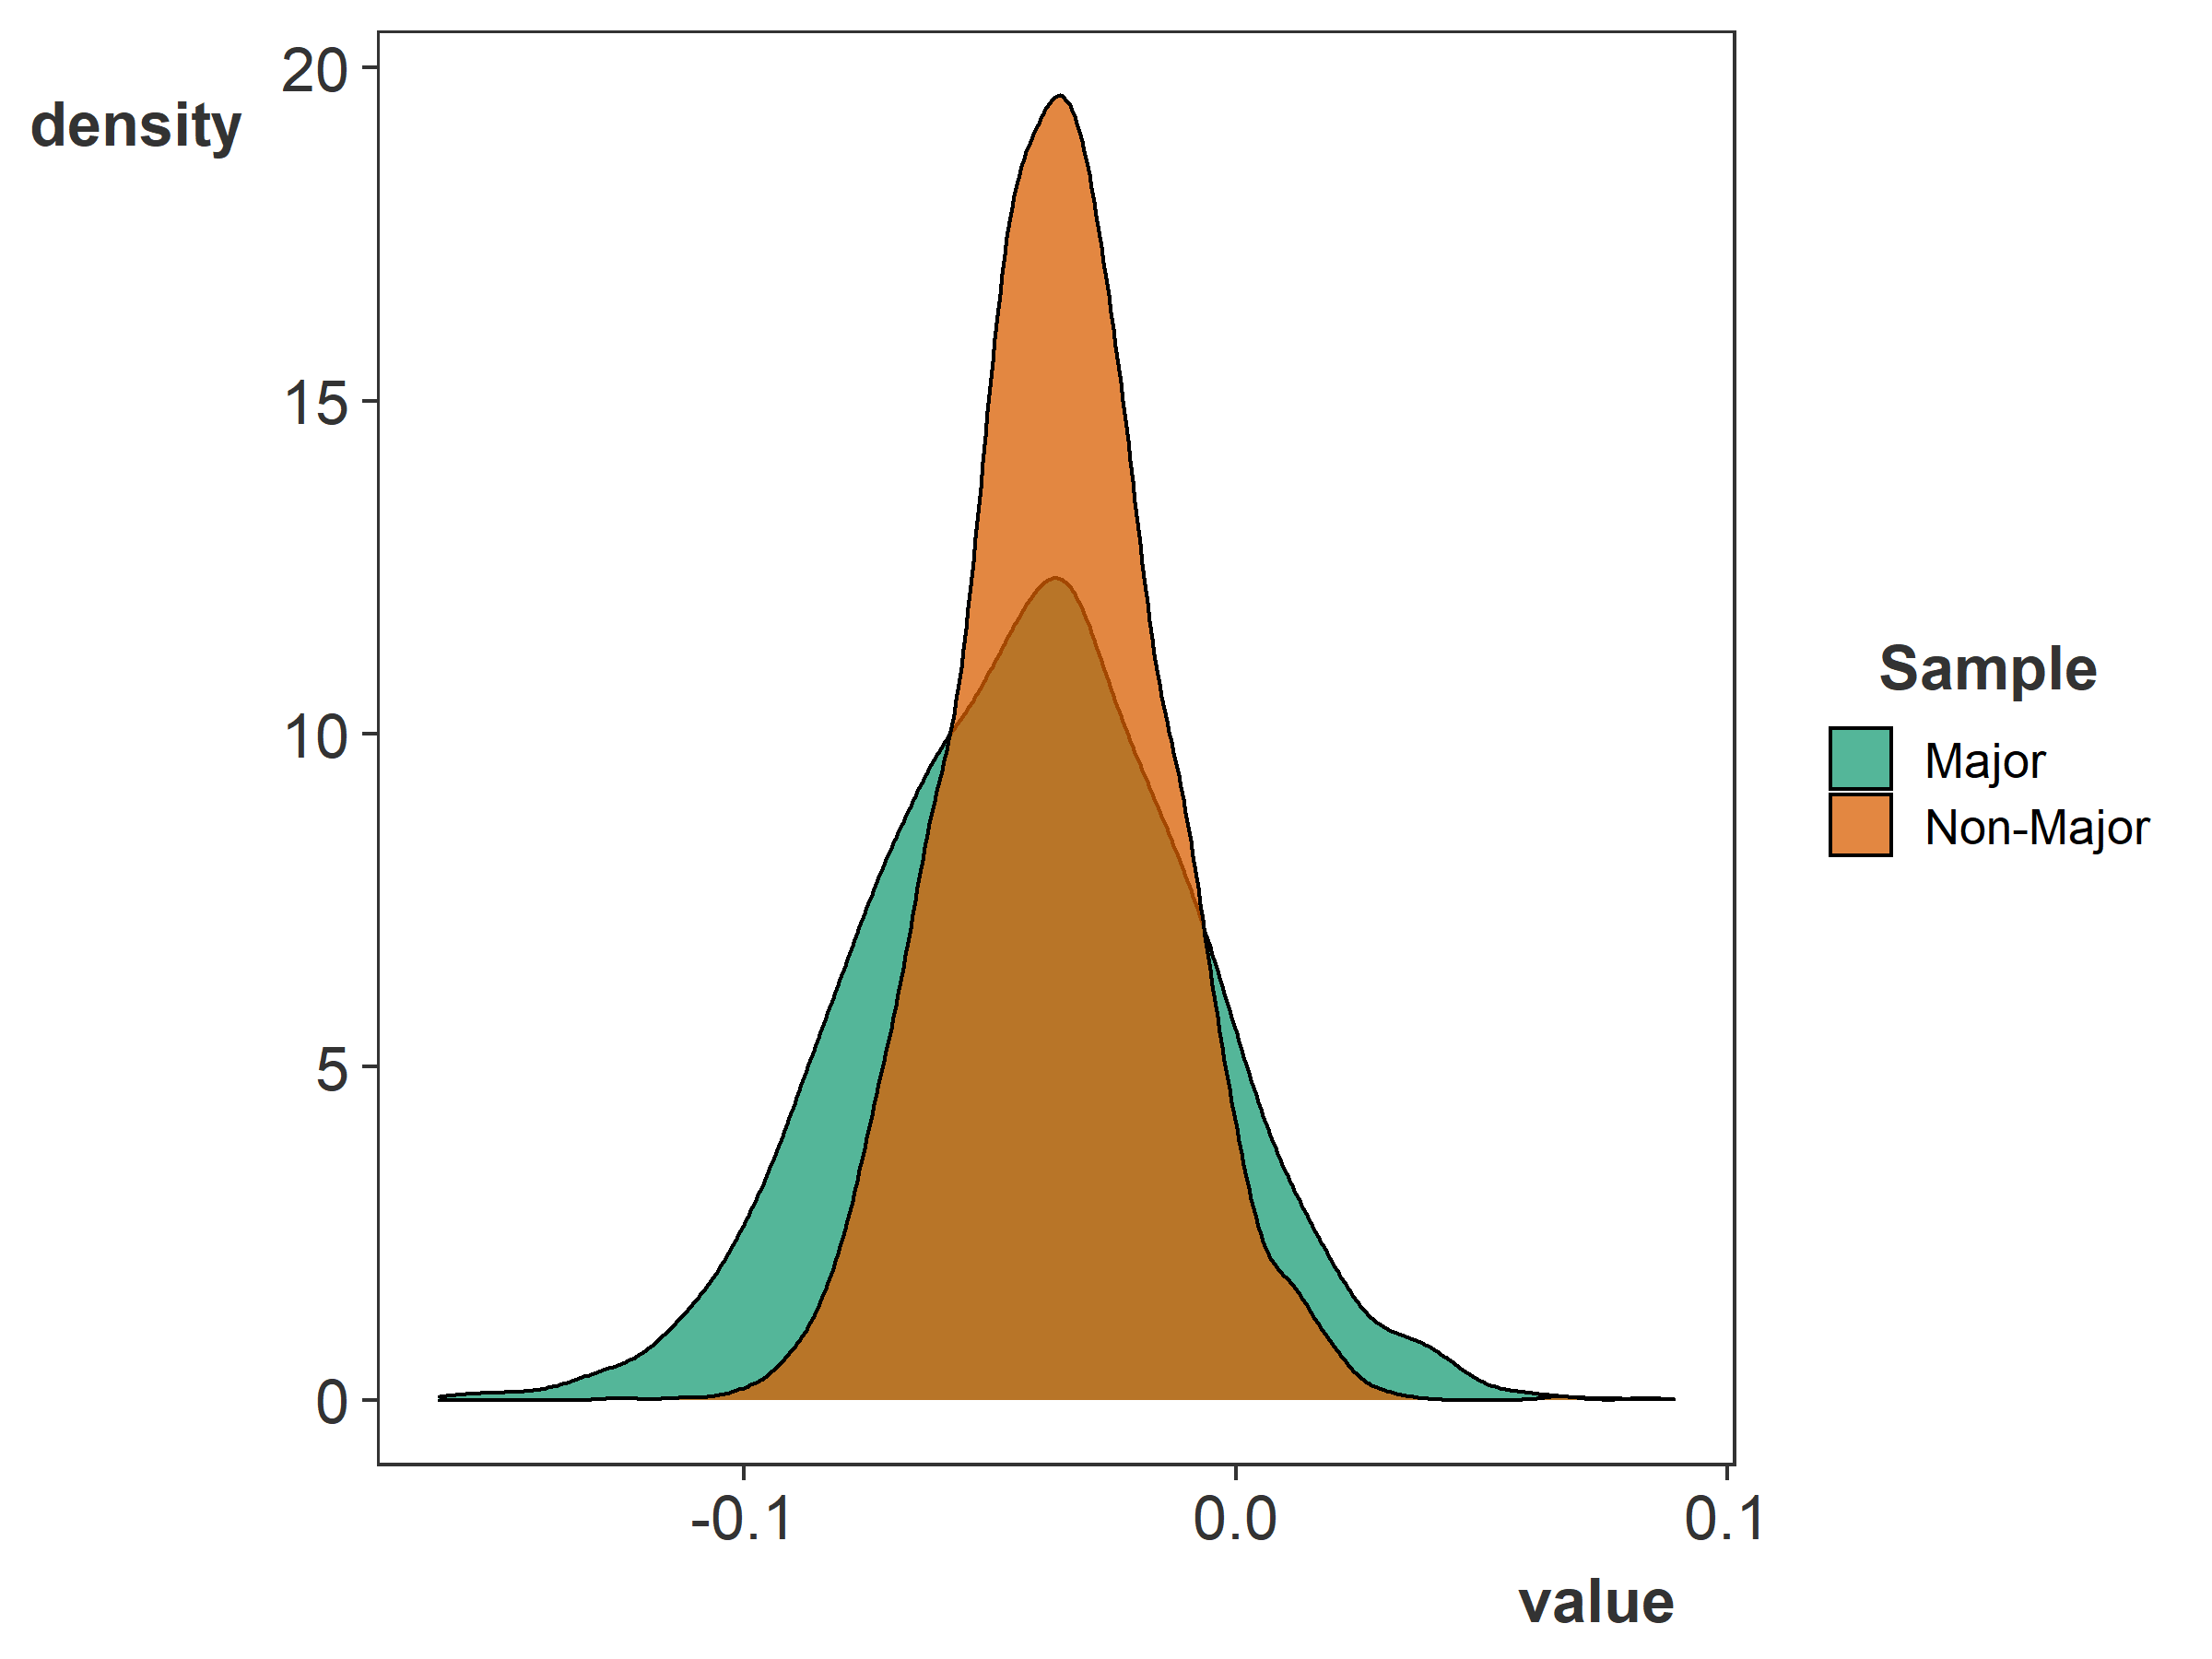
\includegraphics[width=0.95\textwidth]{var-slopes-depth.png}
\end{figure}

\end{frame}


%------------------------------------------------

\begin{frame}{Treaty depth and $\lambda$: Major Powers}

\begin{figure}
	\centering
		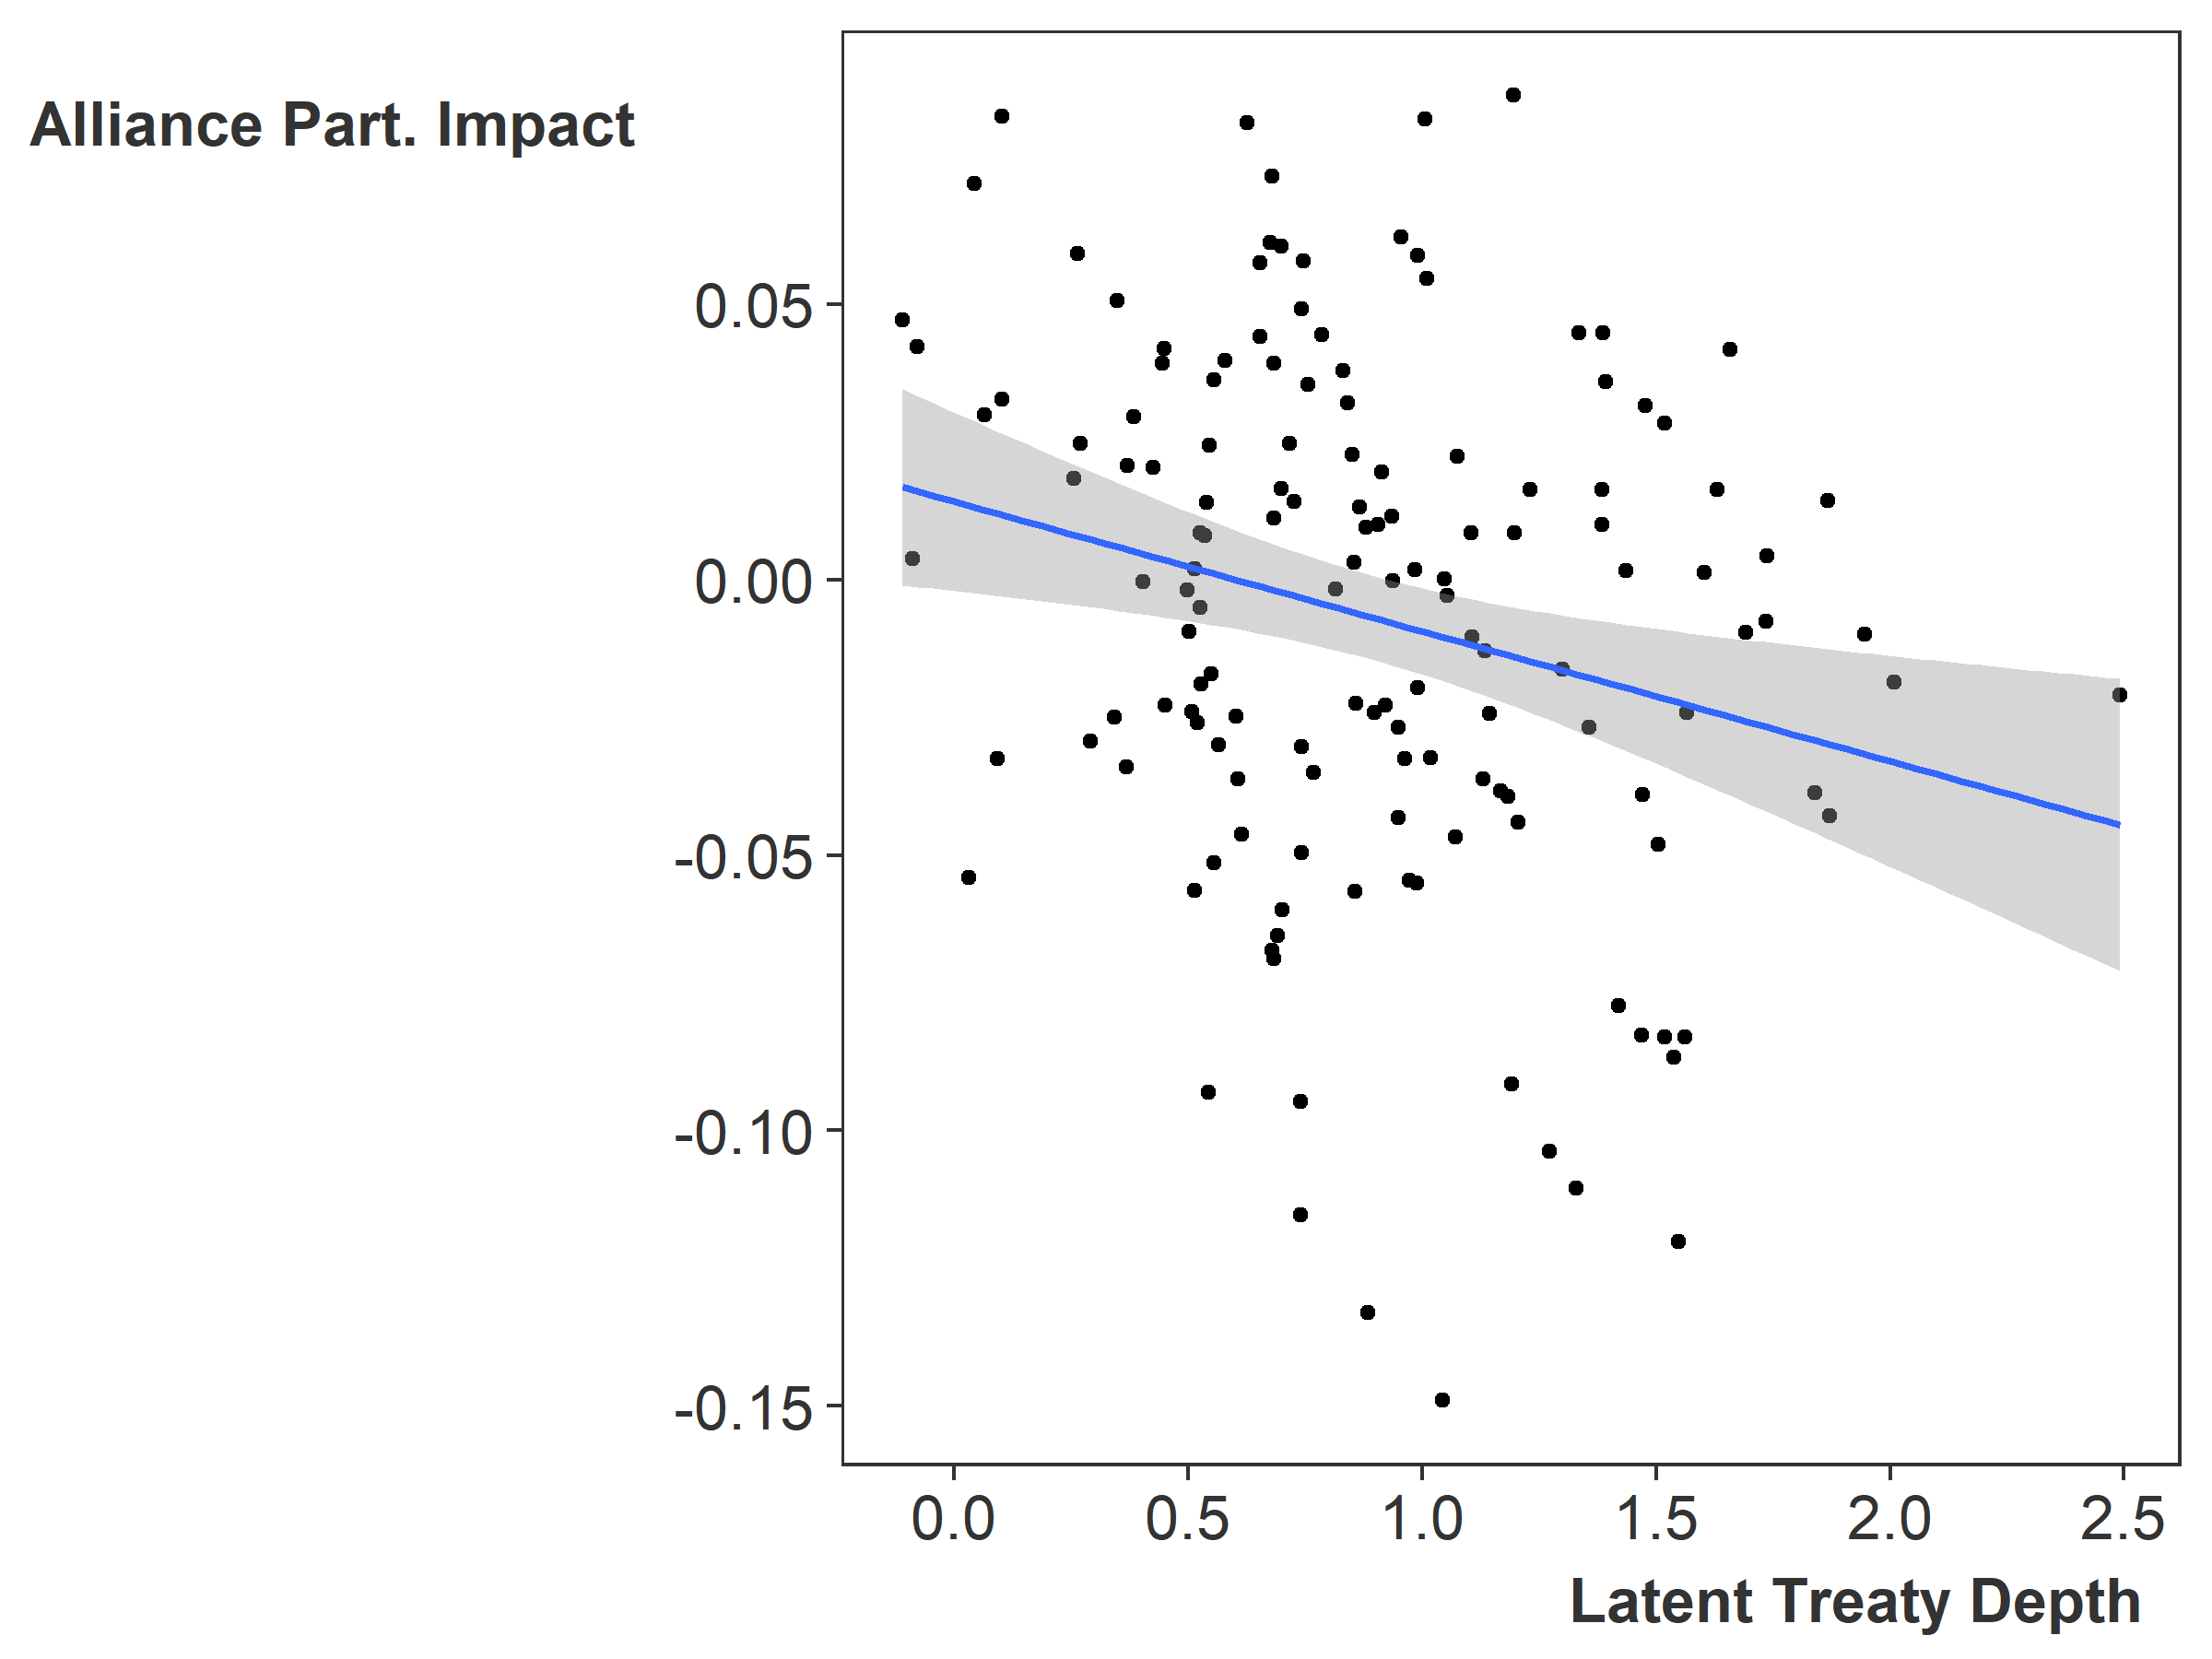
\includegraphics[width=0.95\textwidth]{ld-lambda-maj.png}
	\label{fig:ls-lambda-min}
\end{figure}


\end{frame}

%------------------------------------------------

\begin{frame}{Full Varying Slopes Results}

\begin{figure}[htbp]
	\centering
		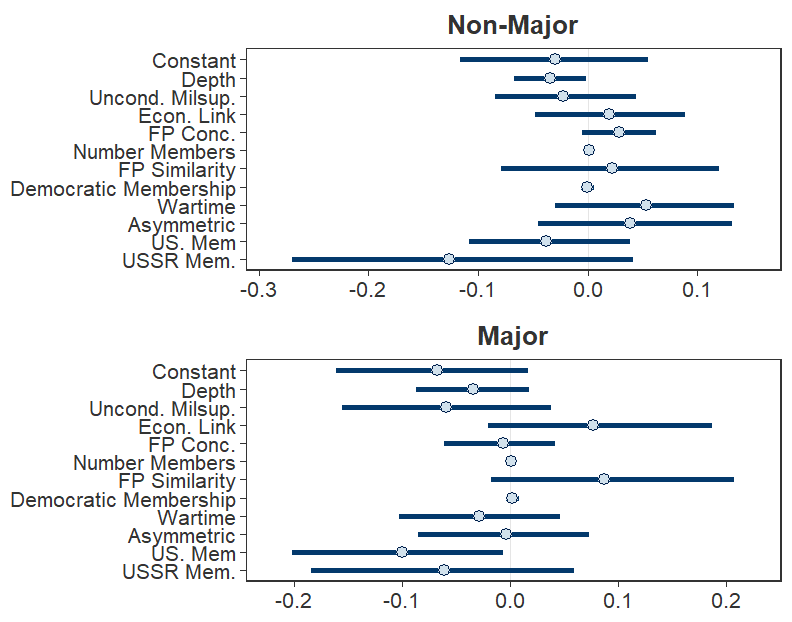
\includegraphics[width=0.95\textwidth]{vs-res-full.png}
\end{figure}

\end{frame}


%------------------------------------------------

\begin{frame}{Alternative Measure of Military Spending}


\begin{itemize} 
\item Nordhaus et al 2012 data: mix of COW and SIPRI- fully rebased
\item 1949 to 2001
\item Same model: use changes in spending instead of growth. 
\end{itemize}

\end{frame}


%------------------------------------------------

\begin{frame}{Alternative Measure of Military Spending: Results}

\begin{figure}[htbp]
	\centering
		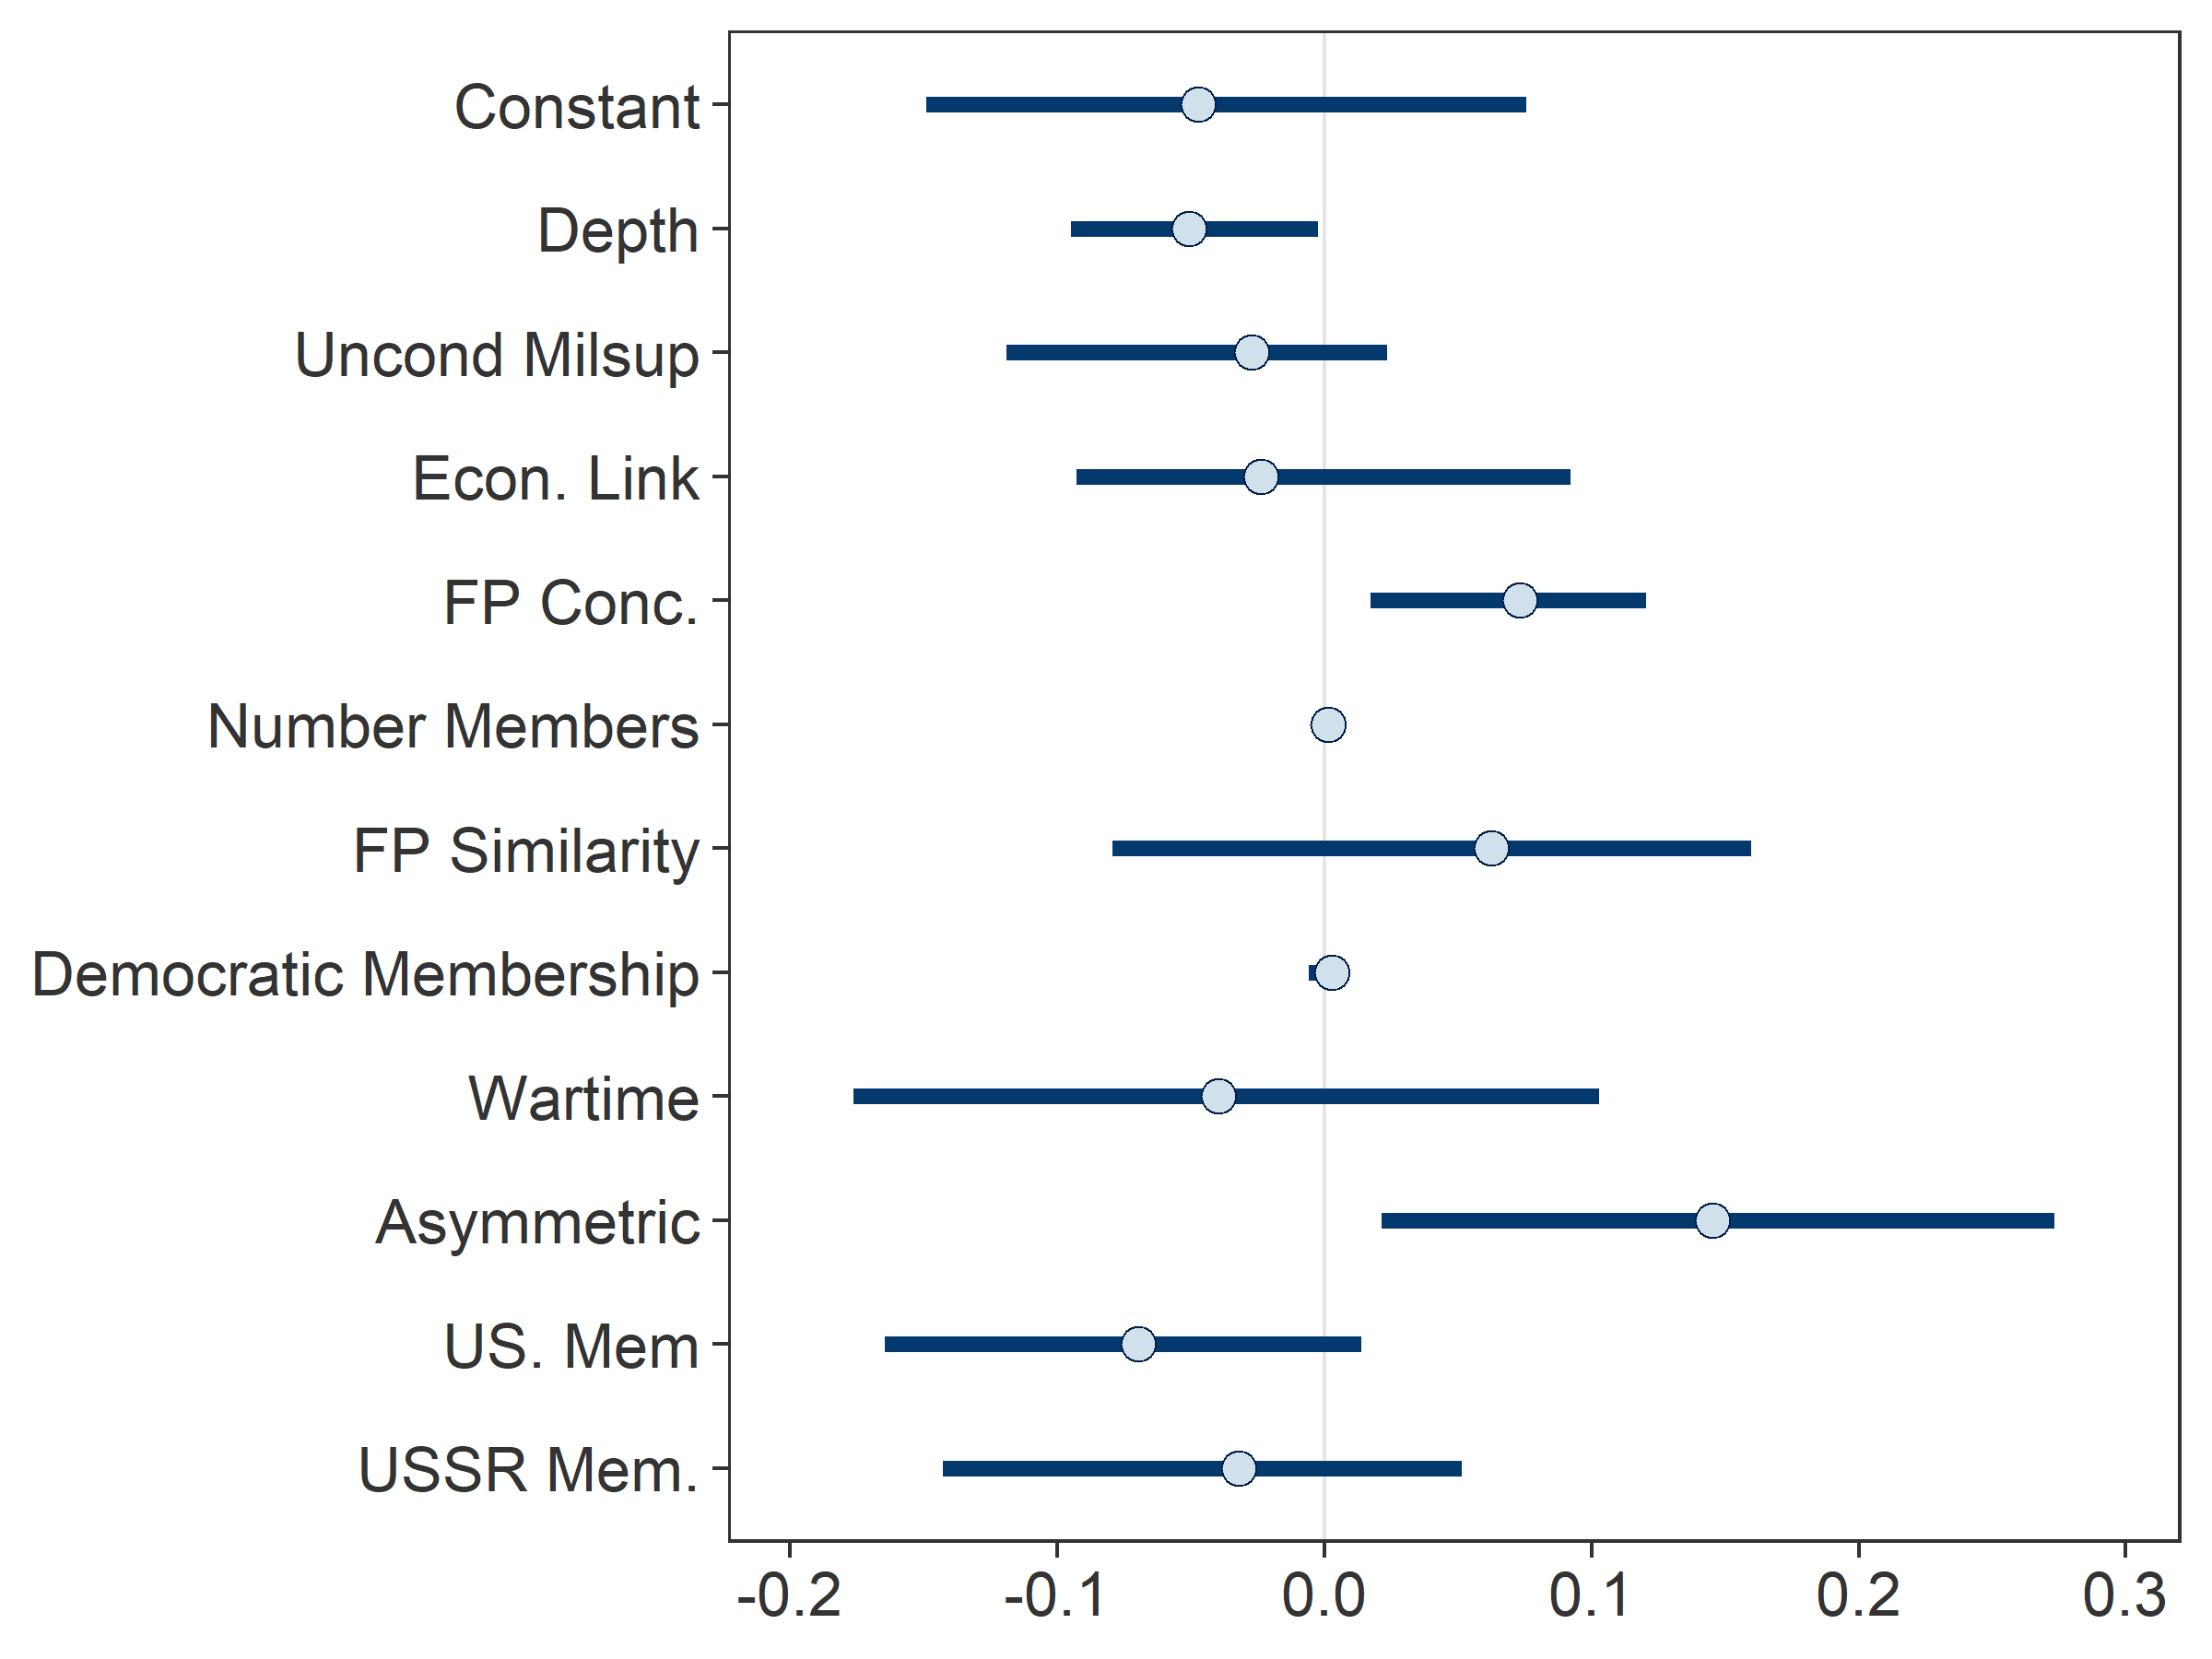
\includegraphics[width=0.95\textwidth]{beta-intervals-post45.png}
\end{figure}

\end{frame}

%------------------------------------------------


\begin{frame}{Single-Level Regression}

Robust regression: Independent variable is average depth of a state's alliances. 

\begin{figure}[htbp]
	\centering
		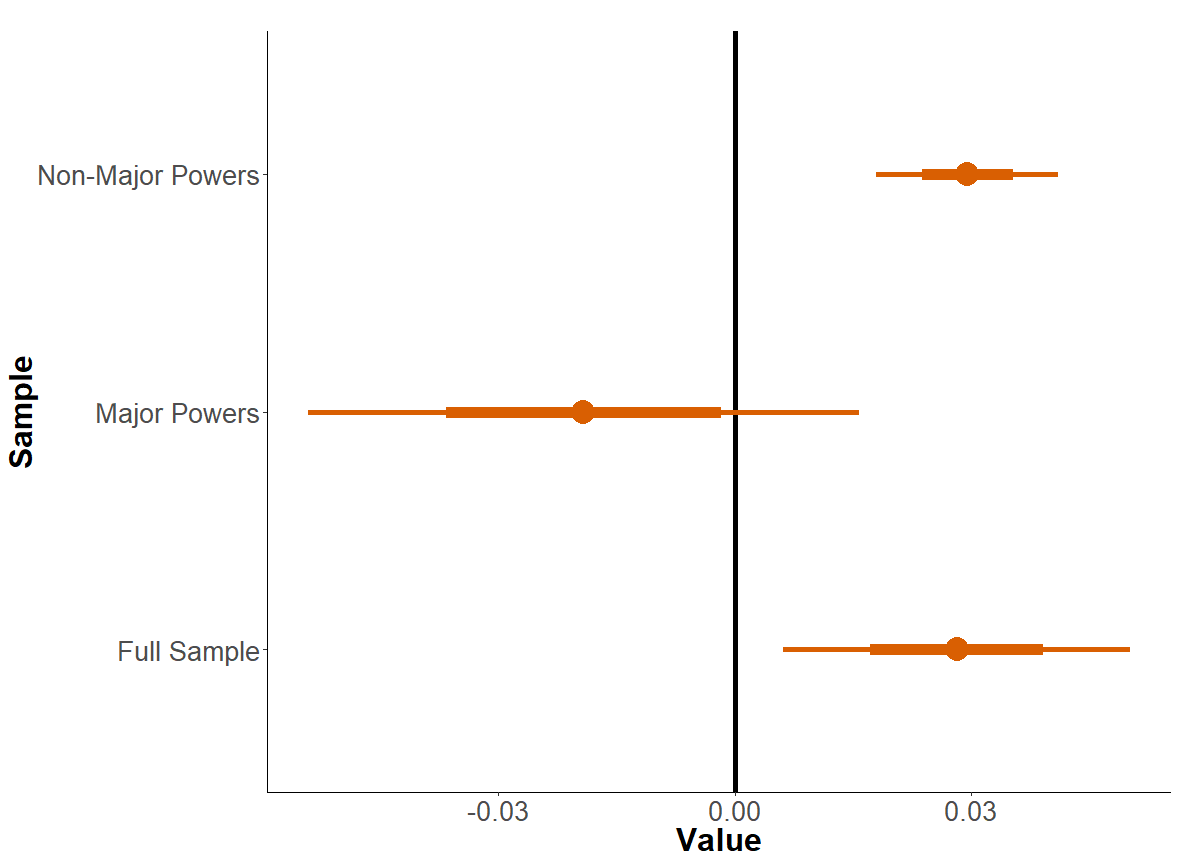
\includegraphics[width=0.85\textwidth]{robust-reg-coef.png}
\end{figure}


\end{frame}


%------------------------------------------------


\begin{frame}{Bounds Analysis of Single-Level Regression}

\begin{figure}[htbp]
	\centering
		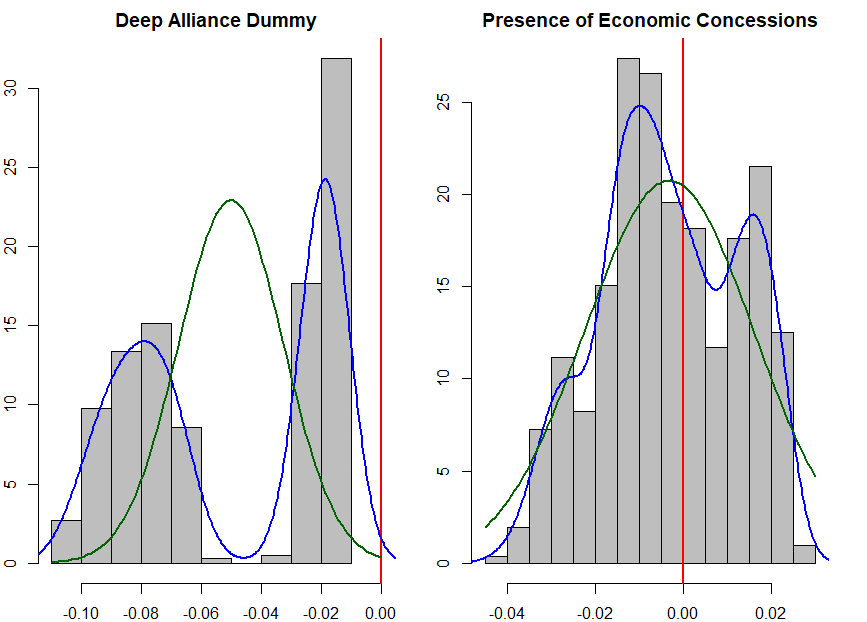
\includegraphics[width=0.95\textwidth]{eba-single-level.png}
\end{figure}


\end{frame}









%----------------------------------------------------------------------------------------

\end{document}